\chapter{Penal Legion}

\begin{wrapfigure}{O}{\figwidth}
	\begin{center}
		
\includegraphics[width=\figwidth]{pics/21/1.png}
	\end{center}
\end{wrapfigure}
Deep inside the sprawling fortress-city referred to by all but the most pedantic of Inquisitors inhabiting it as "Sector Headquarters", No-Longer-Acting-Inquisitor Greg Sargent straightened his orange jumpsuit as the holding room door he'd spent the better part of seven hours staring at finally creaked open. 
The two Inquisitorial Stormtroopers flanking the door, who'd been stuck standing reflexively at attention for the entire time, breathed a little sigh of relief and hastily led the way into the courtroom on the far side.

The four other Stormtroopers in the room relaxed as well as the impromptu poker tournament that'd been occupying the rest of the squad ended without further bloodshed and Aimy, as winner, put Doc and Tink in charge of collecting Twitch. 
While the two of them extracted the demolitions trooper from the pile of furniture he'd squirreled himself away in, Nubby collected the cards he'd "borrowed" and scooted the chair he'd subsequently been cuffed to over to the borrow-ee, who grudgingly uncuffed him. 
The Stormtrooper blinked in confusion as the little trooper sidled off after his companions without returning the cards, or the cuffs for that matter; 
he shared a pained look with the other Stormtroopers as they followed the guardsmen into the courtroom. 
By unanimous silent agreement, the unholy mess that'd once been the court's tastefully-decorated holding room was left for the janitorial staff to discover for themselves.

\begin{wrapfigure}{O}{\figwidth}
	\begin{center}
		
\includegraphics[width=\figwidth]{pics/21/2.png}
	\end{center}
\end{wrapfigure}
As the six Guardsmen quite literally trooped into the courtroom the robe and wig-wearing Inquisitor sitting at its head took them in with the boredly-hopeful expression of someone who was almost done for the day. 
That expression soured as a one of the court's side-doors opened to admit a cart bearing a teetering meter-high pile of binders, folders, loose papers, dataslates, and precariously balanced scrolls. 
With an annoyed glare at the scribe hidden somewhere behind the cart, the Inquisitorial Judge plucked the topmost binder off the pile and cleared his throat.

"Greg Sargent, you and your men stand accused of… parking in a restricted area?" The Inquisitor paused and flipped to the next page, "Failing to vacate in a timely manner?" he flipped farther, "Loading or Unloading a Vehicle in a No-Loading Zone? 
Really?" 

There was a mutter of "it weren' posted or nuthin" from the end of the line of guardsmen and one of the Stormtroopers made a choking sound. 
The Inquisitor shot a glare at both of them as he snapped the binder shut pulled the next one off the pile and cleared his throat again. 
"Greg Sargent, you and your men, you stand accused of Attempting to Bribe a Traffic… Excuse me for a second." The Inquisitor leaned over the side of his desk to glare at the cart-load of files and the figure behind them until he was finally rewarded with a slightly quavery reply. 


"What? 
Do you need help with the long words or something?" 

Ignoring the increasing snickering, and entirely missing the look of confused recognition on three of the guardsmen's faces, the Inquisitor leaned further and gritted his teeth. 
"Why. 
Are. 
They. 
HERE?"

"They're just more of Quercus' idiots. 
Obviously." Sarge's eyes widened slightly, Twitch let out a faint giggle, and Doc abruptly started blushing as a familiar gray-haired woman in adept's robes shuffled out and extracted a leather folio from the middle of the pile. 
"Did you think I'd schedule a real case this late in the day?"

\begin{wrapfigure}{O}{\figwidth}
	\begin{center}
		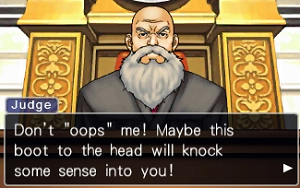
\includegraphics[width=\figwidth]{pics/21/3.png}
	\end{center}
\end{wrapfigure}
The Inquisitor's expression brightened as he opened the folio. 
"I see... 
" he looked back up to the Adept. 
"So all this is just-" he gestured at the teetering pile of documents.

The Adept shrugged. 
"Like I said, idiots."

"Hmmm, quite." The Inquisitor sat up, straightened his wig, and cleared his throat for a third time. 
"Greg Sargent, as servants of a Rogue Inquisitor you and your men are hereby sentenced to-"

"Wait!", interrupted Tink, "You can't just sentence us! 
What about our trial?"

Nubby stepped forward as well. 
"Yeah, you didn' even ask if we was guilty or not!"

The Inquisitor raised an eyebrow. 
 "Are you saying you're NOT part of Inquisitor Quercus' criminally oversized retinue?" 

"Yes!" Tink paused, "I mean no, but we definitely didn't do any of that other stuff."

"An' if we did, we 'ad orders." added Nubby, completely ignoring the boot repeatedly slamming into one of his augmetic shins.

The Inquisitor raised his other eyebrow. 
"Ah, I see. 
So you're saying your Inquisitor ordered you to," he looked down at one of the binders, "Assault, Abduct, and otherwise Obstruct a Traffic Officer in the Performance of Their Duties?"

"Well, he might have..." Tink trailed off as he finally registered the glares of his comrades.

"An' we definitely 'ad orders for the stuff wit the Zoan- OW!" Nubby doubled over as Sarge stepped forward.

'Yes sir." Sarge cleared his throat. 
"Those, uh, traffic offenses were committed in the performance of our duties. 
All of them." 

The Inquisitor turned his gaze to the noncom, who stared not-quite-back with the blankly fixed expression employed by soldiers receiving discipline since time immemorial. 
After several seconds the man shook his head, shot an annoyed glance at the massive pile of files and the Adept behind them, and sighed. 
"Noted. 
Greg Sargent, as servants of a Rogue Inquisitor you and your men are hereby sentenced to Stasis Imprisonment until such a time as the matter of your Inquisitor's loyalty has-"

\begin{wrapfigure}{O}{\figwidth}
	\begin{center}
		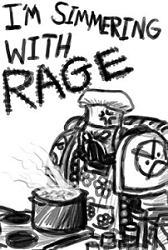
\includegraphics[width=\figwidth]{pics/21/4.png}
	\end{center}
\end{wrapfigure}
Once again the Inquisitor was interrupted, this time by a cough from the Adept and a single envelope being pushed up onto his desk. 
He glared at the elderly woman, who grinned back innocently until he finally sighed and extracted the envelope's contents. 
After a few seconds of reading he paused; 
his eyes skipped down to the signature at the bottom of the letter and then up to scan the line of guardsmen until they settled on the white-haired guardswoman in the center. 
"Oh dear, this is a regrettable situation isn't it?" He glanced to the side, "One I certainly could've been informed of BEFORE the trial started."

The Adept just rolled her eyes and pointed a bony finger at the letter.

The Inquisitor looked back down and continued reading until his expression suddenly cleared. 
"Hmmm, that's certainly an.. 
unexpected suggestion." He tapped his fingers on the letter for a few seconds then looked down to the Adept again. 
"Not a bad one though. 
Surprisingly reasonable all things considered." 

The Adept prodded the massive pile of documents between them. 
"It would save on the paperwork..."

The Inquisitor's lips twitched ever so slightly. 
"And it certainly never hurts to stay on good terms with the sector Militarum. 
Yes..." he sat up, straightened his wig, and returned his gaze to the assembled guardsmen.

 "Greg Sargent. 
This court has decided that, in recognition of you and your men's years of faithful Militarum service and your status as associates of the Lady General Von Humpeding, the charges against you will be deferred indefinitely, and you will be given a chance to redeem yourselves of any crimes you may have committed through service in the Penal Legions. 
Dismissed"

The shocked silence that followed the gavel strike was broken by single, rising growl. 
"That scheming, conniving, two-faced, lying," guardsmen and Stormtroopers alike scrambled back, "RAT-FUCKING-BASTARD, TOLD MY MOTHER!?"

\greentext{>The All Guardsmen Party and the Inquisitorial Penal Legion}


\begin{wrapfigure}{O}{\figwidth}
	\begin{center}
		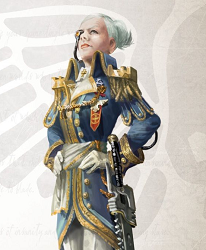
\includegraphics[width=\figwidth]{pics/21/5.png}
	\end{center}
\end{wrapfigure}
So no shit, there we were, being hauled off to die the Penal Legions, just like our old Commissar always said would happen. 
Honestly, it really shouldn't have come as a surprise, especially given Oak's little comment about arranging for us to get a "shorter sentence". 
After all, the average life expectancy of a Penal Legionnaire is probably somewhere between one and zero battles. 
Needless to say, we weren't exactly thrilled with our oh-so-clever Inquisitor, though none of us could quite reach Aimy's level of simmering rage. 


It'd taken three Stormtroopers with shock batons to end our markswoman's little fit; 
she only started to calm down once she got a chance to read the letter that the Adept handed her as she was dragged out. 
We honestly thought the part where her mom said she understood it was all Inquisitorial political bullshit, wasn't her fault, and would always love her were all very touching. 
Less so the bit about how she didn't have to worry about disgracing the Von Humpeding name, because they'd already arranged to have her posthumously disinherited and struck from all family records if she died before the charges were cleared. 
Aimy took some comfort in it at least; 
said it was proof her mother actually wrote the letter herself.

Sarge got an envelope from the Adept as well, but it turned out to just a wad of official paperwork and transfer orders. 
Given the way the sarcastic old bat had choreographed the whole farce we'd sort of expected something more, you know, secret orders-y? 
Maybe a little note explaining just where this top secret evidence-storage facility Oak wanted us to infiltrate was, and how in the Emperor's name we were supposed to accomplish this while stuck in a bloody Penal Legion? 
The only even remotely relevant thing Doc and Tink found in there was a bit saying we had ten days to claim our property out of evidence before it was all incinerated. 
We somehow doubted we'd be given a day off from penal-legioning to do so.

\begin{wrapfigure}{O}{\figwidth}
	\begin{center}
		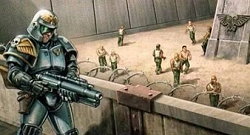
\includegraphics[width=\figwidth]{pics/21/6.png}
	\end{center}
\end{wrapfigure}
We didn't have too much time to dig through the Adept's packet for more clues, or to bitch about how stupid the whole situation was for that matter. 
We'd expected to be shipped across the planet or system to some munitorum depot, but as it turned out the HQ had their very own Penal Legion stationed on-site, presumably to save on gas or something. 
After a short drive, the Stormtroopers hauled us out and we got our first look at our new home: 
"Camp Redemption" as the big sign over the gate declared it, or "The Dump" if you went by the spray paint under it.

Honestly, it didn't really look that bad: 
if you ignored the fact that all the defences were pointed INWARDS it could've passed for pretty much any other Guard camp we'd seen. 
Same prefab buildings, same drill yards full of sweating grunts, same ankle-deep mud. 
Hell, it even had the same smell; 
that wonderful combination of body odor, pit latrines, stale rations, and spilled prometheum. 
Sarge took a deep nostalgic breath, as did Twitch and Nubby, Aimy just made gagging sounds.

Now the camp's occupants on the other hand… We'd apparently arrived right at some sort of muster, but we didn't pay the thousand or two shaved and bomb-collared troopers much mind. 
No, the first thing our trained guardsman senses noticed was the sheer number of Commissars strutting around. 
Your typical regiment, in as much as there is such a thing in the Guard, tends to sport around one Commissar per company, or even less if you were one of them fancy pants nobby regiments; 
we spotted what had to be at least one pointy-hatted bastard per platoon, and that wasn't all. 
Instead of the Arbite shock-squads we expected to be keeping discipline in the ranks, the lanes between each platoon were patrolled by squads wearing the blue-trimmed coats and eagerly homicidal expressions of baby Commissars.

Twitch informed the rest of us that we were all going to die. 
For once, nobody argued with him.

\begin{wrapfigure}{O}{\figwidth}
	\begin{center}
		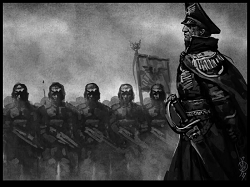
\includegraphics[width=\figwidth]{pics/21/7.png}
	\end{center}
\end{wrapfigure}
Our grim speculation was interrupted by the arrival of one of those cadet-commissar squads, led by a particularly unpleasant looking real one carrying a whip. 
The Commissar, a weasel-faced bastard somewhere between 60 and 600 depending on how much juvenant they'd pumped into him, angrily informed the Stormtroopers that they were late. 
After a bit of confusion about the transfer orders and why in the Emperor's name they'd given them to us, he ordered his minions to just chain us all together and get us in formation; 
he'd process us and send back the uniforms later.

The Legion had almost finished forming up in a platoon-wise grid by this point. 
We were led to an empty spot at the near corner, where Sarge was instructed to stand out as far as the ankle-chain would allow and the rest of us lined up behind him. 
Satisfied that we were capable of standing at parade rest without any motivational whipping, the old Commissar told us not to move or say anything, and stalked off to stand at the head of our column.

The reason for the parade became clear when a Scribe with a dataslate and an especially fancy Commissar (who we assumed was the base Commander) arrived and announced that the Inquisition was looking for volunteers. 
To our surprise, they actually got them, at least at first. 
At the back of our line, Twitch claimed that this was a clear sign that they were drugging the rations. 
Doc, who was in the spot ahead of him, actually took him seriously enough to look around and check for signs in the other Legionnaires, and got reminded of the "no moving" rule by the old Commissar and his whip. 


We watched as three whole platoons of chumps stepped forward were loaded up into transports, followed by two more that were more traditionally "volunteered" by the Commissars, and then Scribe announced that the rest of what his Inquisitor needed were specialists, starting with a demolitions expert. 
The old Commissar checked the papers we'd given him and stepped forward.

\begin{wrapfigure}{O}{\figwidth}
	\begin{center}
		
\includegraphics[width=\figwidth]{pics/21/8.png}
	\end{center}
\end{wrapfigure}
Fortunately for us, the specialist positions must've had slightly higher requirements than "literally the first idiot you find", because the Scribe and Commander came down into the ranks to inspect the candidates. 
They did, of course, start with our end of the regiment, but we didn't have to do anything drastic to get Twitch off the hook. 
All it took was one look at the strung-out demo trooper, his own proud declaration that he didn't just know explosives he SLEPT with them, and a single Ork-related accusation in the Commander's direction for them to decide to move on to the next candidate.

Once the headhunting party passed us we began to notice whispering and occasional movements in the legionnaires around us. 
None of us were close enough to the other platoons to really catch what was going on, aside from it obviously being related to avoiding volunteering. 
Since that old Commissar was far too close and attentive for us to consider shifting closer, we didn't pay any of it much mind until a scuffle in the back ranks of our column drew the Commissars' attention away, and someone behind Twitch muttered "Punch Greg next pass". 
The demolition trooper turned to stare in confusion at leader of the platoon behind him, a large muscle-bound dark-skinned man, and asked who "Greg" was. 
This was apparently not the correct response.

The dark-skinned platoon sergeant, who Twitch was fairly certain hadn't been there earlier, rolled his eyes and repeated himself twice, then made a frustrated noise and finally clarified to "Punch Greg Sargent, your Interrogator, RIGHT NOW." Twitch gave him a fish-eyed look and gestured at the chains connecting his ankles to Docs and the distance to Sarge out in front of the line, eliciting more eye rolling until finally realized what was going on and passed the message on to Doc, then to Aimy, Tink, and finally Nubby. 
The short trooper glanced between Sarge's back and the returning Commissar, and then told Tink to ask "What for?".

\begin{wrapfigure}{O}{\figwidth}
	\begin{center}
		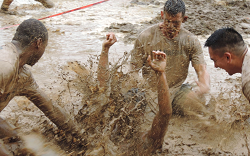
\includegraphics[width=\figwidth]{pics/21/9.png}
	\end{center}
\end{wrapfigure}
The message was passed back down the line to the platoon sergeant, who went bug eyed, but didn't manage to get an actual reply out before the Scribe, just a few platoons away, announced that the last man he needed was someone with a bit of command authority. 
As the Scribe asked the Commander had anyone properly Sergeanty, Twitch abruptly got the point, and passed the message to "JUST PUNCH SARGE DAMN IT!" back up the line, where it once again stalled at Nubby and Tink, who both took one look at the watching Commissar and his whip, and then nominated eachother to do the actual punching. 


The ensuing argument over whether Nubby or Tink would make the less suitable Sarge-assaulter was interrupted by a string of curses and Aimy charging past them at Sarge's back. 
One spot farther back in line, Doc looked down at the chain connecting his ankles to Aimy's just in time to see his feet fly out from under him. 
Nubby and Tink watched as the markswoman slammed face-first into the mud next to them, blinked, and then immediately resumed their argument, paying absolutely no attention to the approaching Commissar. 
Fortunately for the pair, before the actual whipping could start, attention was taken off them by the sudden arrival of the dark-skinned Legionnaire, who's flying tackle hit Sarge hard enough to pull both the arguing troopers down as well. 
 

Twitch, as the only guardsman left standing, watched with a certain amount of satisfaction as the Sarge pulled the Legionnaire off him and did his level best to kill the man until the fight finally broken up by several cadets armed with shock-batons. 
In the silence that followed the exciting round of noncom mud wrestling, the Clerk asked if the Commander if he'd been drugging the rations again.

\begin{wrapfigure}{O}{\figwidth}
	\begin{center}
		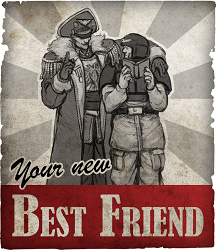
\includegraphics[width=\figwidth]{pics/21/10.png}
	\end{center}
\end{wrapfigure}
The Commander explained to the confused Clerk that they'd discontinued that program for cost reasons and starting fights was a common tactic to avoid getting chosen. 
The dark-skinned Legionnaire had a history of it, especially when it involved his subordinates getting chosen. 
The Clerk digested this, and then said that sort of behavior sounded remarkably leader-like, the Commander grinned and agreed. 
Down in the mud, the Legionnaire started swearing, but quickly shut his mouth as the Commander leaned down and asked if he was refusing to volunteer for Inquisitorial service. 
The man shot a final, exasperated look at us as he was hauled off with the rest of the Inquisitorial volunteers and the Commander and Clerk finally left with the whole parade in tow.

Any relief on our part evaporated as the old Commissar stalked forward again, and had his cadets haul us out of the mud. 
Instead of the expected whipping though, the man gave us a thoughtful look, asked why the Legionnaire would've bothered with us. 
When he didn't get an answer, the Commissar started flipping through our papers (briefly pausing at Sarge's name and rank to look up and ask "Really?") until his expression abruptly lit up with recognition.

The Commissar looked Aimy up and down, and in the most self-satisfied voice we'd heard outside an Inquisitorial briefing, announced that a penal legion was no place for a lady like her, but fortunately the Commissariat would be happy do the Von Humpedings a little favor. 
Aimy's expression conveyed exactly what she thought of his "favor" and where he could shove it, but she still put it into words, just to make sure. 
Unfortunately for the markswoman, it didn't turn out she had much say in the matter, and Cadet-Commissar Von Humpeding was marched off at gunpoint to get a shower and a fancy new hat, while a tech-priest and pair of servo-skulls were brought over to fit the rest of us for some less-fancy explosive collars. 
All in all, she probably got the worse deal.

\begin{wrapfigure}{O}{\figwidth}
	\begin{center}
		
\includegraphics[width=\figwidth]{pics/21/11.png}
	\end{center}
\end{wrapfigure}
One bomb-collaring and servo-skull shave-job later (the part where they'd tattoo our foreheads would apparently wait until deployment), we were standing around wondering just what the hell had happened and if we should've done, well, anything about it. 
Our discussion on the subject was interrupted by someone behind us asking the exact same question. 
We turned around to find a group of four Legionnaires staring at us, Sarge began to say something, and then paused and stared back for a few confused seconds trying to place why the four bald guardsmen we were looking at seemed so familiar, until Twitch and one of the Legionnaires both pointed at eachother and shouted "It's YOU!" and the rest of us (sans Tink) abruptly recognized all four of them as former Trainees from our brief stint as Inquisitorial drill-sergeants. 


It was hard to say who was more surprised, we all just stared at eachother for a few seconds, and then the leader of the group, one of the ex-PDF troopers, laughed, saluted Sarge, and said he never dreamed Oak would send *us* to get them out and we'd better talk to the Interrogator right away. 
At least, as soon as they found him; 
he'd snuck off during the muster to do something or other at our end of the parade grounds. 
According to them, he looked sort of like Sarge but bigger, grumpier, and blacker... 
Had we seen him by any chance? 


\begin{wrapfigure}{O}{\figwidth}
	\begin{center}
		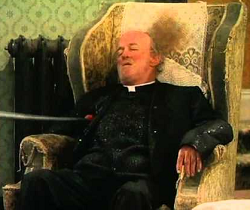
\includegraphics[width=\figwidth]{pics/21/12.png}
	\end{center}
\end{wrapfigure}
The four trainees accepted the bad news about their Interrogator like true guardsmen; 
that is to say with a mixture of swearing, the exchange of a few packs of smokes and ration bars, and a smug "I told you so" from the former scum who'd apparently just won the running death-pool. 
Our pride in them was only tempered by the fact that the agent Oak had apparently sent to help us had just been hailed off to join some sort of Inquisitorial suicide squad. 


They took the news that we had no idea what they meant about "getting them out" and were there for something completely different with a similar amount of cynicism; 
the ex-scribe said it explained a lot, and suggested we get back to their barracks to finish the conversation. 
Doc asked if that was really wise, given how gossipy barracks life can be, but the trainees assured him it was okay: 
they had their very own building separate from the rest of the platoon, just them  and their Commissar, who was "one of the good ones". 
Nubby and Twitch both pointed out that the only good Commissar was a dead one; 
the trainees agreed and said we'd understand when we met him. 


What they meant by that became clear when we entered the lovingly sandbagged and razor-wired prefab, and encountered a rotund red-coated man firmly ensconced in a filthy recliner. 
Judging by the snoring, the man probably wasn't dead, but judging by the thick carpet of liquor bottles on his side of the barracks, he was definitely working on it. 
The Scribe introduced him as Commissar Kelly, gave him a firm poke in the belly, and when he didn't respond, extracted a data-slate from the recesses of the chair and asked whether Sarge wanted to be put down as the new platoon lead or if one of them should do it. 


Nubby, Twitch, and the rest of us admitted that they were right about their Commissar.

\begin{wrapfigure}{O}{\figwidth}
	\begin{center}
		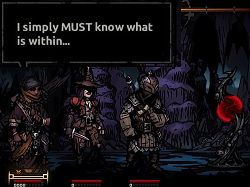
\includegraphics[width=\figwidth]{pics/21/13.png}
	\end{center}
\end{wrapfigure}
Once we'd been officially inducted into the platoon (with Sarge as lead), issued proper Guard fatigues and some disappointingly power-packless lasguns out of a stash behind the Commissar's chair, the trainees brought us up to speed.

As it turned out, the four of them (one PDF trooper,  scribe, cleric, and no-longer-ex-con), hadn't been scooped up as part of the whole Oak thing, they'd actually been enjoying Inquisitorial hospitality since before everything hit the fan. 
Their team had done alright on their first few missions after graduation, as had the other trainees as far as they knew, but a few months back they'd run into trouble. 
The PDF trooper explained that it'd all been because of our training, you see, while our advice about just shooting anyone stupid enough to mess with the blatantly evil eldritch artifacts had served them well, we probably hadn't meant that rule to include Interrogators. 
At least not when there were witnesses around… The good news was that thanks to that decision they'd mostly survived that encounter, and the Inquisition investigators had actually agreed with their decision. 
The bad news was that grunts shooting their superior officers is generally frowned upon, regardless of what organization your in, hence the penal legion.

They'd been in there for the better part of two months, and since regiments were shipped out ever two or three months, that actually made them some of the camp's most senior inmates. 
They'd arrived at the arrangement with their pet Commissar and had been trying to figure out if there was a way to get themselves "forgotten" when the regiment shipped out, and then the Interrogator had turned up and started talking about how Oak wanted to help them escape. 
Not being chumps, they hadn't believed a word of it and told him as much, until the man finally admitted he needed their help for something and would arrange for one of Oak's allies to extract them all together afterwards.

\begin{wrapfigure}{O}{\figwidth}
	\begin{center}
		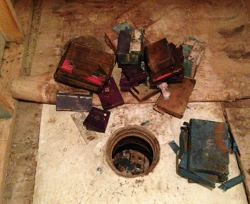
\includegraphics[width=\figwidth]{pics/21/14.png}
	\end{center}
\end{wrapfigure}
Our former trainees had been a bit dubious, but the Interrogator had obviously been some sort of legitimate, because right after he'd arrived the Penal Legion had started being assigned work details around the nearby sections of HQ. 
Somehow he'd gotten their squad permanently assigned to groundskeeping duty at a complex just down the road, and had been devouring their reports on the place's layout and exterior security these last few weeks. 
Of course, being an Interrogator, the man had been tight-lipped about WHY they were doing all this scouting, but given that the largest building in the complex had "Mundane Evidence Storage" written on the front, it didn't take a genius to figure out he was planning some sort of heist. 


Their theory had been reinforced by the contents of the Interrogator's "secret" stash under the barrack's floorboards, which they'd discovered and rifled through about ten minutes after the man had set it up, and happily cracked open to show us. 
Aside from the booby traps (which they declared to be decidedly sub-standard compared to what Twitch had tested them on), the stash contained an Inquisitorial Stormtrooper uniform, complete with a badge identifying the Interrogator as an Inquisitorial HQ guard, as well as some sort of weird dataslate with a badge slot, and several stacks of notes and blueprints focused on (and under) the Evidence Building. 
The final item, tucked in the very bottom of the stash, was a three-ring binder titled "The Loyal Servant of Mars, Mk.121-HS Etheric Variable Discipline Collar: 
Sacred Diagrams and Maintenance Hymnal". 


Tink immediately seized the technical binder, and after a few seconds of perusing, demanded a mirror and a Type-5 Combi-Tool or the closest thing the trainees had. 
The ex-con raised an eyebrow at him and then shrugged, fished a large slightly-bent screwdriver, a cracked shaving mirror, and a few homemade metal shims out from under the Commissar's filthy chair, and told him to go nuts. 


\begin{wrapfigure}{O}{\figwidth}
	\begin{center}
		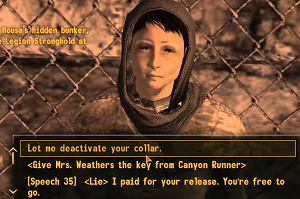
\includegraphics[width=\figwidth]{pics/21/15.png}
	\end{center}
\end{wrapfigure}
After a few seconds of dismayed staring at the proffered tools, Tink huffed, snatched them up and went to work. 
The rest of us watched as the techie began scraping the blunt screwdriver around the seams of his collar in search of something or other, and alternated between cursing at his tools (as well as whichever cogboy had written the manual), and flipping between three different technical diagrams. 


After nearly a minute of this, the former cleric suggested he worry about the collar later: 
the Interrogator had been trying for days and hadn't even managed to get his collar's cover off. 
Tink assured him that it was because the man was a technological idiot who didn't know a diode from a donut, whereas he could read a circuit diagram with both eyes closed and had spent the last year studying technology so advanced it made the mechanicus' simple little toys look like, um, simple little toys. 
The trainee nodded and agreed, and suggested that it might also have something to do with the fact that the manual was for a completely different model of collar than the ones we were all actually wearing. 
One without the special anti-tamper feature, or so he'd heard.

Tink paused, and then very slowly pulled his tools away from his neck and suggested that it might be better if he started with someone else's collar first. 
Everyone in the room took a step backwards, except for Twitch, who suggested that maybe this sort of thing should be left to the demolitions expert instead then grabbed the screwdriver and instructed Tink to hold still. 
Tink decided he'd rather not do this, and darted behind the comatose Commissar with Twitch close on his heels. 


\begin{wrapfigure}{O}{\figwidth}
	\begin{center}
		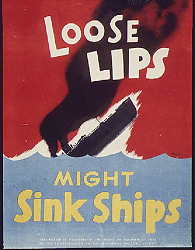
\includegraphics[width=\figwidth]{pics/21/16.png}
	\end{center}
\end{wrapfigure}
While Tink and Twitch bickered, the rest of us perused the Interrogator's notes on the Evidence Building, but it was all disappointingly rough. 
There were several different possible entry points marked on the diagrams, along with little notations about pros and cons, as well as several instances of "ask team's technical/demolitions expert about X". 
Given that said experts were busy playing ring-around-the-Commissar while a harried trainee tried to keep them from waking the snoring man up, we decided those could wait for later. 


The one thing in the notes that really jumped out to us was a complete lack of any sort of objective marker; 
everything was either about getting in or getting out, but not a word on where to go afterwards. 
Noticing our confusion, the ex-Scribe pointed at several strings of numbers and letters jotted along the side of one of the pages. 
He said he was pretty sure the shorter one at the top was the storage unit ID code for Oak's case, and that the rest were the IDs for the individual pieces of evidence he wanted us to steal before his trial.The real question, according to the former PDF trooper, was just what the hell piece of evidence in Oak's case locker was so bloody damning that having it spontaneously disappear would actually improve things? 
Sarge, torn between relief that at least some fragment of operational security had been maintained and feeling like a hypocritical ass, informed the trainees that they really, REALLY, Didn't Need to Know.

Sarge's non-answer was accepted by the trainees with only a moderate amount of grumbling about him having become "one of them", and over the course of the evening a plan was formed. 


\begin{wrapfigure}{O}{\figwidth}
	\begin{center}
		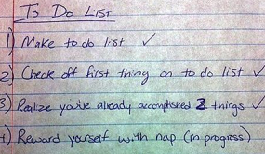
\includegraphics[width=\figwidth]{pics/21/17.png}
	\end{center}
\end{wrapfigure}
Well, it wasn't exactly a plan per-se, more of a chore list. 
For starters, Sarge wanted to have a look at this Evidence building himself, so the trainees did some more fiddling on the napping Commissar's dataslate to get him included on the groundskeeping detail. 
While Sarge was out scouting, the rest of us were to put our heads together on the whole Collar problem. 


After a lot of inane argument, the technical side was assigned to Tink AND Twitch, and the pair were given firm instructions to start by actually reading the outdated manual instead of just looking at the pictures. 
They were going to need some proper tools of course, which was Nubby's job, along with the Ex-Con who said he already Knew Some Guys. 
Finally, since nobody present was willing to let Tink or Twitch fiddle with THEIR collars, Doc was asked to go to provide a corpse or seven. 
The Medic had objected, loudly asking why we expected him to just have a bunch of dead bodies lying around. 
Tink pointed out that A: 
He was an Imperial Guard Medic and B: 
this was a Penal Legion, the only real problem would be finding ones that still had their heads. 
Doc grumpily ceded the point and promised to go volunteer for the Legion's medical corps.

The final chore involved the numbers from the notes, or to be more precise, the very similar ones Sarge vaguely remembered seeing on that little "Please Collect your Stuff" slip mixed in with our transfer orders… the ones that the old Commissar had walked off with. 
According to the trainees, they'd have been filed away in the Commissariat Command Post and none of us stood the slightest chance of getting anywhere near them. 
Luckily for us, we already had someone on the inside, all we had to do was figure out a way to make contact without raising any commissarial eyebrows. 
The trainees asked if we meant that Sister who'd come in with us, and were advised not to call Aimy that to her face if they valued their teeth.

\begin{wrapfigure}{O}{\figwidth}
	\begin{center}
		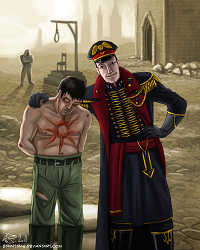
\includegraphics[width=\figwidth]{pics/21/18.png}
	\end{center}
\end{wrapfigure}
The next morning we got our first taste of life in an Inquisitorial Penal Legion. 
They day started off at six with a public execution, followed by a fiery sermon from the Legion's head Priest (some sort of Redemptionist Praecentor we guessed based on all his stuff about cleansing sin through glorious death). 
After the sermon we there was a roll call, in which a slightly disgruntled Cadet stood in for the Commissar we'd been left snoozing in his slightly damp chair, and we moved on to some good old Guard-issue PT and dummy weapon drills, and finally another public execution before lunch. 
Honestly it was all sort of homey; 
just like being back in one of the Training Regiments, if a rather disciplinarian one.

Okay, maybe "disciplinarian" is putting it a bit lightly: 
by lunch the death-count was up to seven, and we were pretty sure the Commissars had some sort of daily competition going on to see who could get the most whippings in. 
Aside from the big public executions (which the trainees said weren't actually a pre-meal tradition, that morning was just busier than usual for some reason), the leading cause of death appeared to be summary execution at the hands of the Cadets for minor, possibly imaginary, infractions. 
This behavior didn't really surprise us, anyone who's met a Baby Commissar could've told you there's a reason why they aren't given authority to shoot Guardsmen until a tour or two has mellowed them out a bit. 
It did strike us as a bit wasteful though, even if Penal Legionnaires were considered even more expendable than your typical Guardsmen (if that's even possible), one had to wonder how they were managing to keep the Legion from dwindling away to nothing before it ever saw combat. 
That little question was answered for us just after lunch,  when an an Arbite convoy escorting four whole busses of new recruits rolled in.

\begin{wrapfigure}{O}{\figwidth}
	\begin{center}
		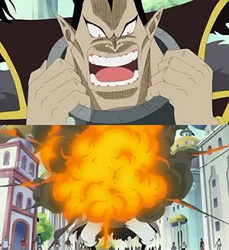
\includegraphics[width=\figwidth]{pics/21/19.png}
	\end{center}
\end{wrapfigure}
According to one of the trainees, the four busses full of new arrivals were the Arbite's weekly delivery of fresh meat. 
See, there were two types of Legionnaires in the camp. 
Unlucky mudfeet and disgraced Inquisitorial agents only made up about a quarter of the Legion, the rest consisted of the hardened dregs of the planet's criminal underworld. 
Unlike us Guardsmen, who accepted our sorry lot fairly easily, the assorted gangers, assassins, heretics, and occasional outright lunatic chafed a little at their new strict military lifestyle, and apparently the more organized members harbored some downright lethal bad-blood for eachother.

Anyway, as the busses unloaded, an entire platoon of Legionnaires jumped some of the new arrivals. 
Some of the Cadets moved in with their shock-sticks to settle things and one of them got a bit too cocky and wound up yanked into the melee, which was when their seniors stepped in and we got to see our fancy Discipline Collars in action. 
All at once, every collar in a large radius started beeping and almost everyone (including us) froze, but the melee's participants were a bit too wrapped in things and didn't stop until their collars went from beeping to an electrical buzzing and they all flopped over into the mud in a twitching heap. 


The Old Commissar strode out of the crowd followed closely by a pair of toadies as well an unarmed Cadet we belatedly recognized as a very stiff and unhappy looking Aimy. 
While a few Cadets pulled their comrade out from under the pile, the Old Commissar fiddled with a fancy dataslate like the one that was kept under our Commissar's chair, and very abruptly three of the Legionaries in the pile didn't have heads. 
Without a second glance, the man turned on his heel and walked off again, only pausing to instruct a squad to "clean that up" and shoot an unreadable glance at Aimy when she began to lag a little behind him. 
The Markswoman immediately sped up and didn't so much as glance in our direction.

\begin{wrapfigure}{O}{\figwidth}
	\begin{center}
		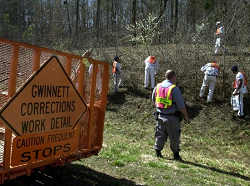
\includegraphics[width=\figwidth]{pics/21/20.png}
	\end{center}
\end{wrapfigure}
Afternoons in Camp Redemption were a little more free than the mornings. 
Most of the Legion got a second round of drills focused on such complex concepts as which way 'round to hold a lasgun, ditch-digging, and how to serve as a human bomb, but as Guardsmen we already knew that stuff. 
The more senior members of the Legion were split up between various work details, which gave us a chance to get started on Sarge's little Chore List.

Sarge's scouting mission to the Evidence Building involved a lot more drain-cleaning and hand-weeding of poisonous xeno-flora than the trainees' description of "light groundskeeping duty" had led him to believe. 
The PDF trainee apologized, saying it varied a lot day to day, since they were filling in for a whole range of servitors that'd been hauled off by the tech-priests. 
When Sarge expressed interest in this, the trainees further explained that it wasn't actually just the Evidence Building's servitors, an entire third of the Headquarters' corpse-bots had been pulled for inspection by a team of Magos'. 
Something to do with the discovery of a shipment of chaos-tainted servitor control units with Inquisitorial markings on some backwater space station… Sarge decided not to ask further questions on the subject.

\begin{wrapfigure}{O}{\figwidth}
	\begin{center}
		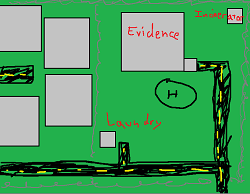
\includegraphics[width=\figwidth]{pics/21/21.png}
	\end{center}
\end{wrapfigure}
During the periods of time when the Cadet overseeing the groundskeeping detail (the same morose-looking one that filled in for the Commissar during the morning) wasn't watching too closely, Sarge got a good look and the Mundane Evidence Building's layout and outer security. 
Nothing really interesting jumped out at him about the building proper, but his attention was grabbed by three smaller buildings sharing its end of the compound. 
The one directly adjacent the evidence building turned out to be a shipping and receiving depot, where the majority of the actual Evidence being stored came in and out. 
Judging by the sweating Inquisitorial Stormtroopers hauling load after load after load of boxes, it was the one menial job in the complex that hadn't been handed off to the Legionnaires.

The second building spotted had an industrial look to it. 
The trainees said it was a plasma incinerator used for general trash burning and the disposal of the various evidence that the Inquisition was done with. 
When the Cadet commissar wasn't nearby, the PDF trooper quietly informed Sarge that the Legionnaire squad currently running it were a bunch of organized locals best not trifled with. 
More importantly, they were also the primary source of contraband in the camp. 


The final smaller building wasn't nearly as interesting, at least according to the trainees. 
They said it was just a laundry processing building, serving both the camp and other Headquarters staff in the area. 
The guys running it were rivals to the incinerator gang, but considerably less organized since two of their leaders had been executed that morning for stealing out of the bins.

\begin{wrapfigure}{O}{\figwidth}
	\begin{center}
		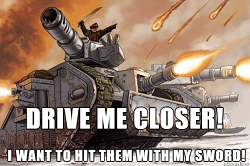
\includegraphics[width=\figwidth]{pics/21/22.png}
	\end{center}
\end{wrapfigure}
Tink and Twitch's assignment was a little less straightforward. 
"Sit around in your barracks, where nobody can see what you're doing" wasn't one of the available duties, so their official job was assisting our Commissar in his functions, both official and bodily. 
Tink had protested and tried to foist the latter part of the job on Doc, but the medic had his hands full working in the camp's medical corps, who'd accepted him without so much a check to see if he knew which end of the scalpel to hold, and immediately set him patching up the constant stream of bleeding Legionnaires sent over from the remedial drills. 
Anyway, fortunately for Tink and Twitch, a few discrete life-support features built into the Commissar's chair handled the ickier parts of their duty, which is why the trainees said they preferred to just leave him in it. 
The Cadet who turned up at the barrack's door pushing a pallet had the same disgruntled expression as the one supervising Sarge's patrol, but he brightened up immensely when Tink and Twitch took it from him and scurried off without asking any questions.

Once the Commissar, who'd attained a vague, profanity-filled semblance of consciousness just after lunch, had been placated with his "morning" drink, and loaded on the pallet chair-and-all, he ordered his new handlers on a lovely little tour of the base. 
Nobody gave Twitch or Tink a second look as they pushed the man around the camp, slurring inarticulate curses at anyone he saw and unsuccessfully commanding the few female Cadet Commissars to service him. 
In fact nobody even gave them a first look, both the Cadets and the other Commissars avoided the trio as much as possible and did their best to ignore them when they couldn't. 
Tink and Twitch quickly decided they liked the man, it was like having their very own profanity-spewing cloak of invisibility, which only occasionally spit on them and threw empty bottles at their heads.

\begin{wrapfigure}{O}{\figwidth}
	\begin{center}
		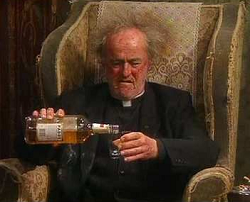
\includegraphics[width=\figwidth]{pics/21/23.png}
	\end{center}
\end{wrapfigure}
The parade wound up visiting pretty much every building in the camp, with the notable exception of the Command Post, which the Commissar informed the pair was full of pissant busybodies unfit to choke on his massive… well, safe to say he wasn't on the best of terms with his nominal superiors. 
From what Tink and Twitch could gather from the little tidbits of sense mixed in with the incoherent ranting, the man had once had a pretty successful commissarial career with some fancy noble regiment. 
Medals, parades, beautiful women expressing their eternal gratitude to their planets noble saviors, and all that stuff; 
right up to the point where literally his entire regiment deserted (NOT the Tau Empire, Twitch checked). 


The man had just came back from a trip to planetary HQ with the regiment's other Commissar and they were gone, gear, armor, tents, camp followers and all; 
nothing left besides an excessively detailed note telling the campaign's senior brass where to stick it. 
Needless to say, said brass had been pissed. 
The Inquisition had gotten involved, things had gotten political, and here "they" were, assigned permanent duty to this shithole. 
Not to the legion mind, but the camp itself, everyone else got out eventually, one way or another, but not him or "that weasel-faced, self-righteous, ass-kissing, ladder-climbing, lying little shit". 
His once solace in life was that our "glorious" deaths would doubtlessly be long, horrible, and probably involve Orks with pointy sticks. 
Twitch wholeheartedly agreed.

Anyway, after a final stop at the quartermasters for as much booze as the harried man running the stores would give him (plus a few extra bottles he commanded his minions to cram down their pants when the man's back was turned), Tink and Twitch were freed to do as much collar-tinkering as they could manage while the old man's increasingly slurred curses transitioned to snores. 
The Cadet never came back for the pallet.

\begin{wrapfigure}{O}{\figwidth}
	\begin{center}
		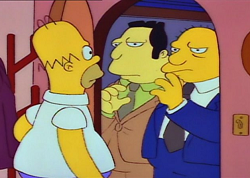
\includegraphics[width=\figwidth]{pics/21/24.png}
	\end{center}
\end{wrapfigure}
Nubby, who'd vanished along with the ex-Con trainee, returned to the barrack after everyone else that evening and brought a set of what looked to be home-made lockpicking tools with him. 
Unfortunately he also brought three Legionnaires, one of which Sarge recognized from the crew working the incinerator, and there was a bit of disagreement on the matter of payment. 
A few bottles out of the snoozing Commissar's stash had originally been offered, but upon arrival the biggest of the three men informed us that the Interrogator had run up a tab and we'd inherited his debt. 
Needless to say, we saw things differently: 
Tink and Twitch were in favor of just killing them, we did have 3 to 1 odds on them and were all armed selection of pokey metal things courtesy of their stop at the quartermaster's office. 
Doc and Nubby were feeling a bit wussier though, especially considering the way we'd seen the old Commissar break up that one fight, so the ultimate decision was left to our fearless leader.

Sarge briefly debated the merits of establishing superiority by punching the biggest thug in the snout, possibly with his augmetic hand, but judging by the trainees' worried expressions it didn't seem like the smartest fight to pick, and anyway, it was a bit early to be burning bridges with our only supplier in the camp. 
After a bit of arguing and haggling from Sarge and Nubby respectively, the thugs were sent off with as much booze as the trainees felt we could slip out of the Commissar's collection without him noticing. 
The three men smugly thanked us for the "interest payment" and said they expected more next week. 
We didn't need the trainees to tell us that the arrangement wasn't going to be a stable one.

\begin{wrapfigure}{O}{\figwidth}
	\begin{center}
		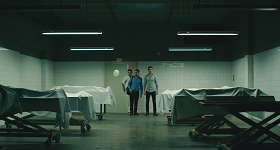
\includegraphics[width=\figwidth]{pics/21/25.png}
	\end{center}
\end{wrapfigure}

Our shaky relations with the local underworld were only a minor concern compared with the looming 10-day time limit on them throwing all our stuff out. 
We weren't sure what Oak would do to us if his super-secret Conspiracy-foiling boxes got thrown in the incinerator, but we were pretty sure death would be a preferable alternative, so it was an incredible relief when we finally got our first real break on the sixth day. 
That morning, thanks to a downright heroic series of fuck-up by the locals during the live fire drill, nearly two dozen legionnaires landed themselves in the base hospital, while another ten skipped straight to the morgue. 
Doc's offer to handle the post-SNAFU cleanup, including the augmetic "recycling", was eagerly accepted by the overworked head medicae.

That afternoon the drunken Commissar's escort was larger than usual, and a bag of tools was crammed under his chair. 
After the mandatory first stops to empty and refill the crotchey bastard, the parade paused at the morgue, where Tink and Twitch split off while Nubby and the ex-Con trainee stayed with the Commissar and kept an eye out for trouble. 
Inside the morgue, Doc had the seven legionnaires who'd died with their collars on laid out and ready, and watched over Tink's shoulder as the techie brought out his tools and announced his intention to start by isolating the primary control board. 
A few seconds of fiddling later, Tink had one of the collar's panels open, exposing a jumble of wires, circuits, shaped charges, and a little boxy-thing which he didn't recognize from the manual, which immediately started beeping. 
Tink managed to duck in time; 
Doc was covered with a light marinade of neck-bits.

While Doc swore and attempted to fish the legionnaire's head out from the table it had rolled under, Twitch seized the tools from Tink and reminded the techie that he'd told him so: 
the first step HAD to be disconnecting the detonators. 
Doc swore again as a second head rolled past him.

\begin{wrapfigure}{O}{\figwidth}
	\begin{center}
		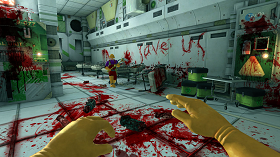
\includegraphics[width=\figwidth]{pics/21/26.png}
	\end{center}
\end{wrapfigure}
Ten minutes and four more headless corpses later, we'd firmly established several things NOT to do, especially in regards to the beepy-box thing. 
Tink was nursing a burned hand and arguing with Twitch over whether they should try wrapping the last collar in the some of scan-proof fabric they'd wrapped the tools in before they made an attempt on the final "volunteer", when the corpse in question abruptly sat up and announced that he actually felt completely fine and would be returning to duty now. 
There was a shocked pause as everyone tried to shift mental gears, and then the man and bolted for the exit. 
None of us had gotten more than three steps before the not-quite-dead legionnaire hit the heavy, metal, and (thank the Emperor) LOCKED fire-exit at a full sprint, and bounced off with a sound like a coconut being hit with bat. 
All three troopers breathed a sigh of relief, only to freeze as someone started knocking on the door from the far side.

Fortunately, the knocker turned out to just be the ex-con trainee. 
Once Doc let him in, he began to ask if we'd set off any alarms, only to break off mid-sentence as he registered the unholy mess of headless corpses, the patina of gore dripping off the walls, ceiling, and all three troopers, and the feebly-twitching legionnaire lying in front of the door. 
The trainee paled, and announced that we were all going to die. 
At Doc's prodding, he expanded, explaining that a posse consisting of the old sour-faced Commissar, his entourage, and the tech-priest in charge of the collars had just left the command building, and he was pretty sure they were coming this way. 
We had just a few minutes to somehow hide the evidence of collar-tampering and get out of here, or they'd have the lot of us up on the gallows before dinner-time. 
Doc whimpered, Twitch swore, and Tink pulled the unconscious legionnaire's pants off.

\begin{wrapfigure}{O}{\figwidth}
	\begin{center}
		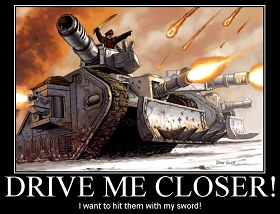
\includegraphics[width=\figwidth]{pics/21/27.png}
	\end{center}
\end{wrapfigure}
Outside the morgue, Nubby noted that the trainee hadn't come back, and the commissarial posse the man had been so worried about seemed to be heading towards the hospital's entrance. 
After briefly debating finding somewhere else to be, the little trooper decided that what was probably needed was good old fashioned distraction. 
He eyed the composition of the oncoming group, and then chair-bound Commissar on the pallet next to him, who'd worked his way through half the bottle of Sacra they'd given him after breakfast to keep him quiet, and then grabbed the pallet's handles. 
As he pushed his cargo on an intercept-course for the posse, he leaned forwards: 
"Eh, uhh, sir? 
I was wonderin, what'cher 'pinion on... 
tech-priests?"

The approaching group saw Nubby and his pallet coming; 
it was a bit hard to miss them, given that the drunken old man riding it was slurring at the top of his lungs about how if he had it his way all those smug metal bastards would be rounded up and shot like the heretics they were. 
His volume only grew as, at Nubby's prodding, he began expounding the various shortcomings of the martian priesthood, ranging from the moral, to the personal, to the sexual, and what he felt should be done about them. 
The group immediately began to curve around the obstacle, only to find Nubby and the Commissar turning to match them, and then turning again as they tried the opposite side. 
The demented game of anti-chicken continued until, at a range of around 15 meters, the ranting Commissar spotted the group's tech-priest, and loudly instructed his minion to push him closer. 
Nubby did as ordered.

\begin{wrapfigure}{O}{\figwidth}
	\begin{center}
		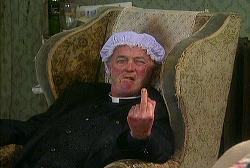
\includegraphics[width=\figwidth]{pics/21/28.png}
	\end{center}
\end{wrapfigure}
Faced with the fearsome might of Nubby's speeding pallet of doom, the approaching Commissar and his cadets abandoned the field of battle and dodged off into the mud next to the path. 
The tech-priest tried to dodge with them, only to find himself back in the line of fire as the white-haired Cadet next to him suddenly slipped on the mud and shoulder-checked him back onto the path. 
The pallet smashed through the cogboy's shins like they weren't even there, because they weren't, the grav plate that'd replaced them bobbed him over the metal edge without it even ruffling the hem of his robes; 
the Commissar riding it on the other hand… 

The now-empty Sacra bottle shattered spectacularly as it hit the tech-priest's metal jaw and the man reeled backwards, only to be brought up short by the liver-spotted hand gripping the front of his robes. 
The four Cadet-Commissars watched as their nominal superior with a mixture of shock, horror, and in Aimy's case, poorly disguised glee, as he drunkenly menaced the terrified tech-priest with the jagged remains of his bottle and Nubby cheered him on. 
Sadly, the show didn't last long: 
Nubby's cheers abruptly cut off as his collar sent a few thousand volts through his neck, and the weasel-faced old Commissar stomped forward and knocked both the bottle and the tech-priest out of Commissar Kelly's hands. 
The chair-bound commissar started to angrily slur something, only to pause as he registered who'd disarmed him, and instead fix the man with a look of immense hatred, which the other Commissar returned in kind. 


After nearly two minutes of mutual death-glaring (which is a lot, at least if you're doing it properly), the more vertical of the pair broke off and shifted his glare to Nubby. 
He gave the still-twitching trooper a few stress-relieving kicks to the ribs, instructed one of his flunkies to load him onto the pallet and return both him and the Commissar to our barracks, and resumed his march towards the hospital.

\begin{wrapfigure}{O}{\figwidth}
	\begin{center}
		
\includegraphics[width=\figwidth]{pics/21/29.png}
	\end{center}
\end{wrapfigure}
When the Commissar and his posse finally entered the morgue, with their bolt-pistols drawn and a worried-looking Head Medicae bringing up the rear, they found a blood-spattered Doc standing over a similarly stained pile of clothing and augmetic body-parts. 
The Medic snapped to attention, attempted to salute, nearly brained himself with the severed metal arm he was holding, and (following the first rule of survival-oriented soldiers since time immemorial) Kept His Damn Mouth Shut. 
The Commissar eyed him for a second, and then swept his gaze around the morgue, taking in both the bloody mess and the complete lack of any other living legionnaires in the room. 
He motioned to the tech-priest, who waved around something that looked like a cross between a dataslate and an auspex, and then pointed at the pile next to Doc. 


At the Commissar's signal, Aimy moved forwards, dug around in the bloody mess, and after the slightest pause, extracted one of the detonated collars from it. 
The Commissar fixed Doc with an absolutely menacing gaze, and asked what in the Emperor's name he thought he was doing here. 
Doc didn't need to feign the panic in his voice as he began rattling off the Generian Regimental Regulations (5th Edition, of course) on the Post-Mortem Recovery of Wargear, Augmetics, and Personal Effects of Greater than Fifty Thrones Value. 
The Commissar's expression didn't change, but the cadets behind him shared a disbelieving look and the Head Medicae let out a pained groan. 
Aimy, catching on immediately, summoned every ounce of incredulous disgust she could muster as she asked if he was really stupid enough to try and salvage a live discipline collar. 
Doc just blinked at her, and claimed that it hadn't been THAT hard, at least not after he'd figured out you could skip the bonesaw if you set them off first by poking the "beepy-bit" with a scalpel. 


\begin{wrapfigure}{O}{\figwidth}
	\begin{center}
		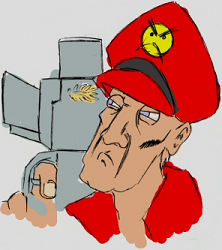
\includegraphics[width=\figwidth]{pics/21/30.png}
	\end{center}
\end{wrapfigure}
Inside the large medical waste bin at the far end of the room, Tink, Twitch, and the trainee listened as the Tech-Priest ranted at the Head Medicae about agreed upon procedures and standards of training for all medical corps personnel. 
Any relief on their part quickly evaporated as the Commissar told the arguing pair save it for later and asked the Tech-Priest whether he was sure there weren't any other legionnaires present. 
All three troopers in the bin tightened the strips of scan-proof cloth they'd torn off the tool bag and wrapped around their collars, and hoped like hell that Tink actually knew what he was talking about for once.

Out in the room, Doc suffered a moment of heart failure as the tech-priest waved around his auspex-slate and announced that there was some interference from all the screamer-signals, but he was picking up at least two still-active collars in the room; 
the Commissar immediately tapped something on his own dataslate. 
Doc dropped to the floor, thrashing and clutching at his sparking collar, and so did the not-quite-dead legionnaire on one of the nearby tables. 
The Commissar pondered this new development for a second, then shot the man in the head with his bolt pistol. 
There was a slight rustle from the bin as Twitch misinterpreted the sound, but fortunately nobody noticed and Tink and the trainee managed to hold him down.

The Commissar, once he'd deactivated the shocker, gave Doc a brief, but incredibly condescending lecture on penal legion regulations vis-a-vis corpses and collars, and how the latter were the sole responsibility of the Commissariat. 
He wrapped it up by punching a command into his dataslate and holding his thumb against the biometric reader on it, and then freshly-decapitated legionaire's collar popped open. 
His little demonstration done, the Commissar began to collect his posse, only to pause and shoot a look at where Aimy was still standing next to Doc. 
In a thoughtful voice, he asked if they knew each other.


\begin{wrapfigure}{O}{\figwidth}
	\begin{center}
		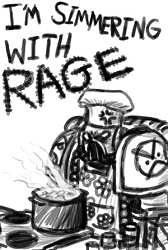
\includegraphics[width=\figwidth]{pics/21/31.png}
	\end{center}
\end{wrapfigure}
Doc's "No" was cut off by Aimy's "Yes", after a slight pause, in which the Commissar gave Aimy a very piercing look, the markswoman explained that they'd just arrived in camp together. 
The Commissar stared at her some more, and then shrugged and announced that she wouldn't have any problem handling his discipline them. 
Aimy, without even the slightest hesitation, turned and popped Doc in the jaw hard enough to knock the medic across the nearest table. 
The Commissar just sighed, shook his head, and held out his whip to her as his Cadets dragged Doc outside towards the parade-ground.

When Sarge returned from his groundskeeping detail, he was less than thrilled to find Doc lying on his stomach with a pile of inexpertly-applied bandages on his back, Nubby with a similar set around his burned neck, and Tink and Twitch arguing with each other about who'd been wronger. 
The only real bright side of the whole thing, aside from nobody actually getting killed, was that Doc managed to get in a brief word with Aimy as she cut him down from the whipping post. 
He was able to direct the markswoman towards the camp chapel, and that evening the ex-Cleric managed to finally catch her alone long enough to relay our urgent request for our mislaid transfer paperwork. 
At Tink's request the trainee also asked if she could get us one of those fancy collar-removing dataslates, but Aimy said that wasn't going to happen: 
while they had her dressed up like a red-coat, they sure as shit didn't trust her like one. 
Not only did the old Commissar have his minions following her and snitching on her every action when she was out of his sight, she wasn't even allowed to have a weapon and he personally frisked her every time they left the command building. 
Honestly that last bit surprised the hell out of us, not because it didn't make sense, but because none of us ever imagined Aimy had the self control not to at least try to kill the unpleasant old bastard on the spot.

\begin{wrapfigure}{O}{\figwidth}
	\begin{center}
		
\includegraphics[width=\figwidth]{pics/21/32.png}
	\end{center}
\end{wrapfigure}
Anyway, Aimy claimed that even if she could score us a Commissar's dataslate, they could only remove collars with the biometric authorization of their owner, and she didn't see herself getting out the door with an unconscious red-coat draped over her shoulder. 
The best she might be able to do would be a Cadet's dataslate, but that was what our Commissar had, so the Cleric trainee told her not to bother. 
So no fancy dataslate for us, but she promised to get the orders to us in time for our infiltration, which Sarge's "plan" said was four days off. 
And yes, the term was definitely "plan", because even Twitch and Nubby's most harebrained schemes had more structure than what our fearless leader was proposing.

Okay, maybe that's a bit harsh, Sarge's favorite all-purpose command "handle it" only appeared at five points, but that's still five more than anyone who's about to BREAK INTO AN INQUISITORIAL FACILITY would ever say they're comfortable with. 
The general theory was to start by taking the majority of the Interrogator's notes on entry-points, especially all the details about the defunct tunnels under that whole compound, and chucking them in a bin. 
We figured that if the man felt putting on a Headquarters-Security uniform and going in the front door was good enough for him, it would be good enough for all of us too. 
Of course we were shy at least four of said uniforms, but we figured a visit to the compound laundry would fix that, problem was, the fellows working the place were beyond useless. 
We'd known their recent run-in with the Commissariat would leave them cagey, but the second Nubby even floated a suggestion their way, they'd all clammed up and threatened to call the Commissars. 
Sarge's personal visit to their building and offer to swap duties with them, which had been met with outright hostility and paranoid accusations of working for one of the other crime families, had rounded off the general cavalcade of failure that was the sixth day.

\begin{wrapfigure}{O}{\figwidth}
	\begin{center}
		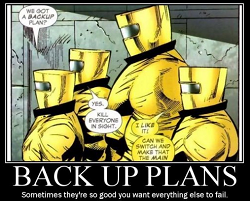
\includegraphics[width=\figwidth]{pics/21/33.png}
	\end{center}
\end{wrapfigure}
So we needed a bunch of uniforms we didn't know how to get, and to remove a bunch of collars we didn't know how to remove, and that was still before we even got in the door. 
Once inside and passed the manned checkpoint that was the main barrier to entry, Tink and the ex-Scribe were fairly certain we'd be able to move through the majority of the facility using the security badges everyone who went in there seemed to be wearing. 
We just had to get one, somehow, and use the card-reading datalsate that'd been in the interrogator's stash to copy it onto a few other cards, also acquired "somehow". 
The incredibly vague plan after that was to walk around, potentially kidnap some clerk and force him to disgorge some directions, and eventually find wherever they'd shoved our gear and Oak's boxes. 
The one actual firm part of the whole thing was that since that was the day they'd be throwing our stuff out, nobody should blink when we showed up and grabbed it. 
Now, what they'd think when we rolled up to Oak's evidence-locker…

Anyway, skipping over the question of how we'd get access to the evidence for what seemed to be the biggest case in the sub-sector, at least the Interrogator's notes had some reassuring bits in them about security screamer-tags only being applied to the contents of evidence boxes. 
Theoretically, we would be able to go in and swap Oak's boxes with some of the containers in his locker, and leave with the leftover empties without setting off any alarms. 
Then it would just be a matter of taking all of our stuff out the shipping entrance under the guise of incineration, and then just cheesing it back to… somewhere. 


So, yeah, safe to say were a bit dubious. 
Still, though, if Oak had told the truth about them putting everything we'd had on the Arbite vessel into storage, once we got to our locker we'd have weapons, grenades, and three entire crates of high-explosives to work with... 
and in our experience that could "handle" pretty much anything.

\begin{wrapfigure}{O}{\figwidth}
	\begin{center}
		
\includegraphics[width=\figwidth]{pics/21/34.png}
	\end{center}
\end{wrapfigure}
Time being limited and the idiots on laundry duty being uncooperative, the next day we launched what could be called a hostile takeover. 
Emphasis on the hostile part. 
Given their paranoia they were probably expecting something, but we didn't show up at their barracks in the middle of the night with a bunch of lead pipes and making faux-subtle comments about unrefusable offers: 
that's civvy thinking there. 
Any proper soldier can tell you that even the most low-key training drills offers an amazing array of ways for someone to check themselves off the active-duty roster, especially if their comrades are willing to give murphy a little hand. 


First there was the catastrophic knee dislocation during PT, then the unfortunate incident where two legionnaires fell into the razor-wire they were practicing clearing, and the poor fellow who's collar malfunctioned during the mud-crawl. 
Obviously this all caused a bit of distraction in their platoon-mates, which was probably the reason that three more of them managed to misplace their assigned dummy-weapons. 
The Commissar in charge of their platoon seemed willing to go easy on them, but at the arrival of a bunch of cadets, one of whom promptly began asking pointed questions about the disciplinary regulations, he decided to make a bit of an example. 
That afternoon, after the whipping and publicly announced reassignment back to remedial drills with the latest bus-load of FNGs, the Commissar in charge of the work detail assignments asked for volunteers with prior laundry experience. 
For some reason, nobody aside from us stepped forward.


\begin{wrapfigure}{O}{\figwidth}
	\begin{center}
		
\includegraphics[width=\figwidth]{pics/21/35.png}
	\end{center}
\end{wrapfigure}
Laundry duty involved a disappointingly high amount of actual duty, largely due to the Commissar that'd previously managed the detail sticking around to make sure we didn't burn the place down or anything. 
The man actually seemed pretty impressed by our well-honed stain-scrubbing and underpants-starching skills and willingly turned command over to the morose cadet officially overseeing us at the end of the shift. 
Still though the way he was looking over our shoulders while we worked was enough to discourage us from trying to pocket anything. 
It wasn't a total waste though, we were at least able to ascertain that suitable numbers of HQ Stormtrooper uniforms came through for us to borrow a few, and we did indeed spot one with an ID badge carelessly left still-attached. 
That specific uniform wound up mis-filed back into the "IN" pile.

Upon our return to base, we received even more good news: 
during their medically-mandated light Commissar-sitting duty, Doc and Nubby had come up with an actual non-suicidal idea for dealing with the collars. 
Well, actually it was Nubby's idea mostly, but that didn't NECESSARILY rule it out. 
While sitting around, watching the old Commissar work his way through the fourth bottle of the day, Doc had regaled Nubby with an in-depth, profanity filled, account of Tink and Twitch's decapacitation experimentation. 
At the point where everyone except the unfortunate medic had hidden in the bin, Nubby raised the question whether we REALLY needed anything better than the scan-proof fabric. 
After all, if the stuff could block that tech-priest's scanner, wouldn't it also block the Commissars' data-slates and whatever they used to watch for escapees? 
Doc's excitement over this novel new idea soured somewhat when he was nominated to be the test-subject while Nubby played mad-scientist with the old Commissar's dataslate.

\begin{wrapfigure}{O}{\figwidth}
	\begin{center}
		
\includegraphics[width=\figwidth]{pics/21/36.png}
	\end{center}
\end{wrapfigure}
So, after a few hours of painful experimentation, at least on the testee's part, Nubby and Doc delivered the verdict that an anti-scan scarf would definitely, totally, 100% do the trick. 
At least, if we kept the heist to under 20 minutes that is, because after that point the collar would start loudly beeping and administering increasingly powerful shocks until the covering was taken off it. 
Doc estimated, using some completely arbitrary math, that if we really had to we could stretch it to a whole hour before the shocks became incapacitating, and maybe another half hour after that before they became fatal. 
The ex-Scribe trainee corrected this figure down to just 40 minutes, because at that point the collar would just give up and detonate, he'd seen it happen to some of the legionnaires that the Commissars had assigned to run messages, back before the Inquisition got tired of cleaning up the bodies and told them to knock it off. 
Doc got really pale at this and decided to leave further testing to Tink and Twitch (who were both less than thrilled to be shown up by Nubby of all people).

Our moderately-productive of possible excuses for why a squad of Inquisitorial Stormtoopers would show up to the Evidence Building wearing a collection of scarves, neckerchiefs, or other neck-covering attire was interrupted by someone knocking on the barracks door. 
Sarge's disgust was palpable when he opened it to find the same big stupid bastard that'd shaken us down for booze a few days ago, this time backed up by a full eight flunkies as well as the badly-limping boss of the former laundry-gang. 
The lead-thug glowered at Sarge in a manner that was probably supposed to be threatening, but mostly came off as constipated, and informed us that we owed his "new best buddy" an apology. 
A material one.

Sarge barely managed not to roll his eyes as the idiot rubbed his fingers and thumb together in front of his face.

\begin{wrapfigure}{O}{\figwidth}
	\begin{center}
		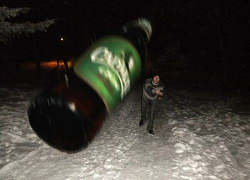
\includegraphics[width=\figwidth]{pics/21/37.png}
	\end{center}
\end{wrapfigure}
Once again, we were stunned by just how suicidally stupid these guys were. 
It wasn't just that they showed up at our door to try and intimidate us with what was, at best, roughly equal strength, they also had the absolute gall to demand not only the hand-over of laundry-detail, but the old Commissar as well. 
Sarge did actually TRY to talk them out of it (even if it was mostly just to buy time). 
He began to say something along the lines of "just give us three more days to enact our secret Inquisitorial mission and it's all yours", but managed to catch himself in time and converted it to a vague request to work the job until all the old laundry crew was healed. 
This, coupled with some alcoholic reparations, the return of most of Tink and Twitch's tools, and the Owing of a One, seemed like a more than reasonable offer to us. 
Even the laundry-boss seemed to think so, judging by the way his expression fell and he started backing up when the big thug rejected it. 
Sarge's expression, on the other hand, didn't even change as his sucker-punch hit the idiot in the jaw. 


Surprisingly, the lead thug didn't fall down, at least not until one of the full liquor bottles the rest of us had been collecting for the bribe hit him square in the nose with every ounce of force Doc's throwing arm could muster. 
That shot was followed by two more bottles courtesy of Tink and Nubby, which hit the nearest two flunkies in the stomach and groin respectively. 
Twitch's bottle had a little flaming rag stuffed in the mouth and all things considered, it was probably a good thing that it just bounced off his target's head with comical thunk as opposed to shattering like he'd intended. 
Those thugs remaining upright immediately drew a combination of shivs, pipes, and clubs and started to advance, only to scatter backwards as Sarge kicked their leader down the short stairs like an especially ugly bowling ball. 
The arrival of the four trainees on both their flanks was a bit redundant.

\begin{wrapfigure}{O}{\figwidth}
	\begin{center}
		
\includegraphics[width=\figwidth]{pics/21/38.png}
	\end{center}
\end{wrapfigure}
The one-sided scuffle was brought to an abrupt halt by a stream of slurred profanity, an (empty) bottle to the back of Tink's head, and a long shock from all of our collars as the old Commissar woke up and demanded to know who'd been stealing his drinks. 
There was a brief pause, in which the few thugs still capable of fighting visibly debated whether to try and take us while the collars had us down, and unanimously decided to just cheese it before any real red-coats showed up. 
All weapons were immediately stashed and all un-broken bottles (including Twitch's still-burning one) were retrieved from mud and returned to their rightful place next to the old Commissar's chair. 
Tink exchanged an open one with a straw in it for the man's dataslate before he could shock us anymore. 
As the thugs staggered, crawled, or were dragged back off to whichever barracks they'd come from, the former laundry-boss (who'd made the wise decision to just stand very still at the back of the group and see how things worked out) sighed and advised Sarge to be very careful before limping off after his new "friends". 


Despite what certain superiors of ours have said about our mental faculties in comparison to those of a waterlogged gerbil, we knew a hint when we were explicitly handed one with a little red bow on top. 
That's why the five unfamiliar legionnaires lounging around the nearest bathrooms the next morning were so surprised to find all nine of us treating Sarge's morning shit as a group exercise. 
Similar groups were dissuaded during roll-call, service, and PT, as well as a larger group who seemed to be aiming to eat their breakfast next to us until the combined weight of Sarge and Twitch's concentrated glaring convinced them to find something else to do.

\begin{wrapfigure}{O}{\figwidth}
	\begin{center}
		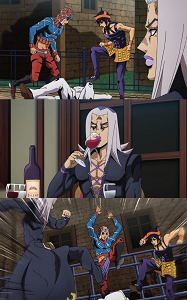
\includegraphics[width=\figwidth]{pics/21/39.png}
	\end{center}
\end{wrapfigure}
The goons obviously could take a hint too, because when we got to training field, we encountered a pair of Cadets splitting incoming legionnaires up into new squads for morning drills. 
When the two baby Commissars spotted us, they immediately began homing in and started to bark off what sounded like carefully memorized group assignments, only to pause as none of us moved and they belatedly registered the snoring old Commissar we'd decided to bring with us. 
Sarge casually informed them that we had orders to stay as a unit, and asked if they wanted to have a word with our Commissar about changing that. 
The two cadets blanched, shared a look, and then left without saying anything more.

The downside of bringing the Commissar with us was having to literally carry him, the chair, and the pallet through a full morning of drills, which made us a bit of a sitting duck. 
Aside from the occasional barrage of rocks or mud and unsuccessful attempts to sic other Commissars on us, the chief hazard was periodic attempts to sneak up and snatch or shank someone, which is a bit hard to pull off in an open-bloody-field, especially when one of the targets is a professional paranoid. 
Still though, had to give them points for persistence, most folks would quit after seeing a comrade lose BOTH eyes to crazed, fork-wielding demolitions trooper…  

There was a brief lull during lunch, followed by one last attack by a lone legionnaire who attempted to grab Sarge in the chow line. 
At least, we assumed it was an attack, just, like, a really half-assed one… fortunately the guy only received a little tap to the nose and a light round of kicking before the trainees pointed out that he wasn't affiliated with any known crime family, and mostly just ran messages for people. 
After some awkward sorries, a few bandaids, and some apology-booze from under the Commissar's chair, we received a note from Aimy directing us to meet her the following evening and collect our orders.

\begin{wrapfigure}{O}{\figwidth}
	\begin{center}
		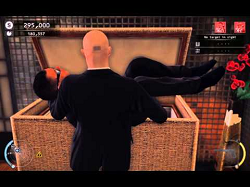
\includegraphics[width=\figwidth]{pics/21/40.png}
	\end{center}
\end{wrapfigure}
The afternoon was blissfully shanking-attempt free. 
There was some concern about the Commissar-watching portion of the team, as well as what might happen to our barracks while we were away, but a deal was worked out with the two depressed Cadets who actually handled all the Commissar's duties, which entailed one of them accompanying their boss and Twitch during his daily walk while the other managed our laundry detail, in exchange for the ex-Scribe trainee doing the day's paperwork. 
By the end of our shift, Nubby's increasingly filthy legion-issue jacket contained three ID badges as well as some promisingly scarf-like bits of clothing, and a test run was made to both the front and freight entrances to the Evidence building under the guise of an unscheduled uniform delivery. 
Rather worryingly, both runs pushed the twenty-minute mark without even actually getting past security.

That night The Plan was revisited, and we came to the uncomfortable conclusion that, unless Tink and Twitch suddenly figured out how to get our collars off, we were going to need to bring one of those Commissar dataslates on the mission with us to periodically reset their timers like they did on work-details. 
This wasn't a problem in and of itself, we had one of those dataslates just lying around, the real issue was that it needed to be periodically "refreshed" by it's designated user via the slate's biometric scanner. 
We fervently hoped Aimy was going to be able to grab a slate and join on the mission, because the only other option involved an unconscious "volunteer" and a laundry hamper, which we were pretty sure would raise some eyebrows at the security checkpoint. 
In retrospect, this might've been a bit of an optimistic take on things...

\begin{wrapfigure}{O}{\figwidth}
	\begin{center}
		
\includegraphics[width=\figwidth]{pics/21/41.png}
	\end{center}
\end{wrapfigure}
The following day went well, suspiciously so in Twitch's opinion; 
the rest of us were just glad not to have any new crises crop up on the day before our mission. 
The drunken old Commissar was brought along to drills again, but aside from a few Legionnaires obviously keeping tabs on us, there was no sign of the opposing force and things went smoothly. 
Or at least as smoothly as a round of field exercises performed while carrying a belligerent, hungover old man with the power to administer shocks directly to your spine COULD go. 


The real good news was when we managed to turn up two more badges in the incoming laundry, one of them belonging to a Stormtrooper Sergeant who we'd seen on duty at the Evidence building. 
Counting the one in the Interrogator's stash that brought us up to six, enough to get all of us (plus Aimy or one of the Trainees) past the automated portion of the building's security. 
Well, at least if Tink was right about the card-slate's ability to, as he put it "clone the creds", otherwise the majority of our little strike force would probably be facing some pointed questions about why someone whose badge granted them access as a Nutrition Technician was trying to enter an evidence storage building. 
There was also the slight issue of the names and pictures physically printed on the cards, but having done our share of gate-guard duty, we were fairly certain that nobody ACTUALLY looked at those. 
Probably.

In any case, we had enough cards, and while we had our Cadet overseer distracted (see: 
napping for half the shift), an entire hopper-load of Stormtrooper uniforms (complete with helmets and assorted neckwear) was crammed behind a dryer. 
With the scan-proof scarfs Tink and Twitch had made, a little pouch of supplies made from the last scraps of the fabric, and a set of vaguely official-looking orders drawn up by Doc and the ex-Scribe, the physical prep was done. 
All that was left to do was meet up with Aimy and hope like hell she had our intel.

\begin{wrapfigure}{O}{\figwidth}
	\begin{center}
		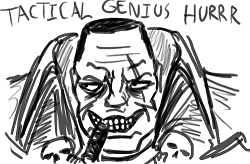
\includegraphics[width=\figwidth]{pics/21/42.png}
	\end{center}
\end{wrapfigure}
The note that Aimy's messenger had passed us said she'd be in one of the storage buildings near the Commisar-y end of the base, half an hour before the evening lockdown. 
Being a bunch of suspicious bastards, we'd scouted the location, double checked her note to make sure that the handwriting matched and there weren't any subtle "the Commissariat is onto us" hints, and had brought our entire force along (Commissar included) just in case it was all a cunning trap. 
The good news was it wasn't, the bad news was that this was just because it was an extremely un-cunning one.

We spotted the large cluster of aggressively nonchalant Legionnaires, loitering in the general vicinity of our destination, from halfway across the compound. 
The big dumb bastard sitting on the building's front step was just a redundant redundancy. 
It belatedly occurred to us that firstly, passing secret notes and arranging clandestine meetings is exactly the sort of thing that the criminal underworld is known for, secondly, there might've been a thing or two we forgot to tell Aimy about our current situation, and finally, unless there was a second female cadet commissar with sororitas-white hair, she'd just entered the building. 
A brief confab was held (which mostly consisted of everyone taking turns blaming each other) and then Nubby, Twitch, and two of the trainees broke off to loop around while Sarge led the rest of us right into the hornet's nest.

The Big Familiar Goon gave a solid attempt at a shit-eating grin when he saw us, but the two black eyes, broken nose, and missing teeth made it a bit hard for him. 
He settled for some sullen glaring and a slurred command for the rest of us to stay put while Sarge was invited inside for a "liddle chad wid da Bosh".

\begin{wrapfigure}{O}{\figwidth}
	\begin{center}
		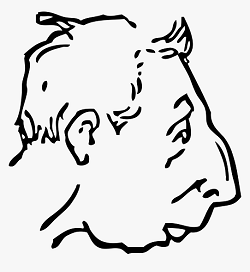
\includegraphics[width=\figwidth]{pics/21/43.png}
	\end{center}
\end{wrapfigure}
The small-ish Guard-issue prefab storage shed was, well, a Guard-issue prefab storage shed. 
It had a floor, walls, boxes, shelves, and (because this WAS a penal legion after all) a bunch of locking metal grates that completely failed to deter anyone armed with a screwdriver, thin piece of metal, or sufficiently strong stick. 
The sign next to the door sporting the words "Thieves Will Be Disemboweled With An Entrenching Tool" was presumably a more effective deterrent. 
Even the table bolted in the middle of the floor was Guard-issue, as were the little folding chairs around it, and the two goons flanking the entrance, and especially their freshly-sharpened entrenching tools. 
The at-least-half-Ogryn guarding the far door was starting the push it though, and while Aimy was technically the definition of Guard-issue, the small dapper man sitting at the table with her, sporting a striped suit and a silenced autopistol, most definitely wasn't.

The Mob Boss, because there was no imaginable way the man could be anything else, gave Sarge a look that would've been intimidating if A: 
Sarge hadn't spent the last few years in Inquisitorial service, and B: 
the man had a chin. 
Like, at all. 
It was just a steady, regular slope from his little mustache to his abnormally large Adam's-apple. 
It was amazing. 
The only thing harder than not staring was not laughing, neither of which are smart when the other guy has a gun and you don't. 
So, in a quiet sort of desperation, Sarge dropped the man from his awareness, and plopped into the free chair across the table from Aimy. 
In a tone of forced chattiness, he asked how the Markswoman's day was going, Aimy rolled her eyes.

>"Oh, you know, sitting around, being the bait in this half-assed trap, because some stupid ass dipshit couldn't bother to tell me they'd started a fucking gang war with the chinless wonder over here."

\begin{wrapfigure}{O}{\figwidth}
	\begin{center}
		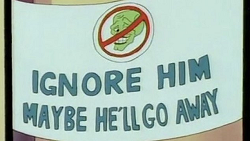
\includegraphics[width=\figwidth]{pics/21/44.png}
	\end{center}
\end{wrapfigure}
The silence that followed Aimy's little remark was a choked one, quite literally in the case of one of the goons behind Sarge, whose face was screwed up into something resembling a felid's anus. 
The Mob Boss attempted to simultaneously glare at both Aimy and the unfortunate goon, but even if he could have pulled it off, the delayed basso "hur, hur, hur" from the half-Ogryn ruined it. 
In an attempt to regain some semblance of control over the situation, the man slammed his autopistol onto the table, rounded on Sarge, and began to bark a question at the noncom. 
For his part, Sarge took one look at the Mob Boss, felt his eyes drag inexorably towards the area where the man's chin wasn't, and abruptly turned back to Aimy to loudly ask if she'd heard we'd gotten assigned laundry duty again.

Whether it was an effort to help Sarge in his moment of desperation, or just sheer desire to talk to someone who wasn't wearing a stupid pointy hat, Aimy responded with some inane chatter about a cadet commissar who'd somehow managed to attach a bomb-collar to himself, and the pair started trading camp gossip in the best tradition of Guardsmen everywhere. 
The Mob Boss and the assorted goons just sort of stared, obviously unsure of how to handle being blatantly ignored in favor of anecdotes about what Nubby found in the dumpster behind the quartermaster's tent. 
Eventually though, the conversation meanedred to the topic of the transfer orders Aimy had been asked to procure and where they'd wound up; 
the markswoman jerked a thumb at the big dumb goon and the grimy wad of papers in one of his fists, and asked what was so important about them anyway. 
Unfortunately, the Mob Boss took this as his cue.

\begin{wrapfigure}{O}{\figwidth}
	\begin{center}
		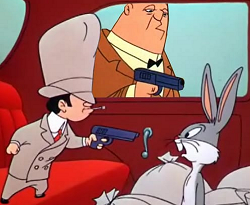
\includegraphics[width=\figwidth]{pics/21/45.png}
	\end{center}
\end{wrapfigure}
In an attempt at a tone of smug authority, the Mob Boss announced that he was deeply interested in Sarge's answer as well. 
What possible reason could there be for a washed up ex-guardsman to be secretly meeting with Commissar Sourface's favorite pet? 
Sarge ignored the question, but raised an eyebrow at the word "pet". 
Aimy didn't actually respond, but her expression clearly conveyed her complete lack of desire to pursue the subject; 
instead she asked whether it was true that Twitch had tried to stab her messenger to death with a plastic spoon. 
Sarge began to explain that it was actually a fork, at which point the Mob Boss's patience finally ran out and he screamed at both of them to JUST SHUT UP.

After a few seconds of hyperventilating, the chinless Mob Boss made a visible effort to reclaim his whole suave villain persona. 
He announced that if we weren't willing to talk, then they'd better just have a look and see what was so important about the papers Aimy had been carrying. 
Lacking a suitably big and swivelly chair in which to lean back and menacingly tent his fingers, the mob boss settled for tilting his folding chair as far as it would go. 
He gestured at his goons with one hand, while using the other (the one with the LOADED GUN in it) to steady himself against the table.

There was a brief pause while the assorted goons waited to see if their boss was going to accidentally shoot someone, and then a second pause as the Big Dumb Goon drew out a rather grimy wad of papers and visibly balked at the sheer amount of words on them. 
With a deeply furrowed uni-brow and one finger moving along the page, the big goon began laboriously reading off the four page standard Administratum boilerplate at the head of our transfer orders. 
The Mob Boss sighed, started to raise his palm to his face, nearly tilted over backwards, and grudgingly yelled at the goon to skip ahead to the part where it said WHY we'd been transferred to the penal legion.

\begin{wrapfigure}{O}{\figwidth}
	\begin{center}
		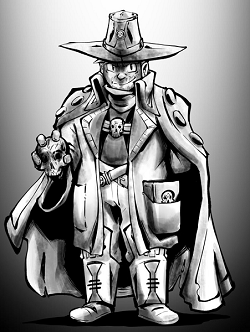
\includegraphics[width=\figwidth]{pics/21/46.png}
	\end{center}
\end{wrapfigure}
In some ways the chinless Mob Boss was more clever than, well, everyone else we'd met (which is honestly pretty sad when you think about it). 
See, instead of shrugging off the concept of a bunch of guardsmen being sent to an INQUISITORIAL PENAL LEGION for TRAFFIC TICKETS, he started asking questions. 
Specifically, after his broken-nosed goon slurred out the fourth count of "Failing to Vacade in a Dimely Manner", whether there were any NON-TRAFFIC related convictions.

Both Sarge and Aimy struggled to keep their poker faces in place as, after nearly a minute of searching, the goon read off "Aiding and abeding da Rogue Inquisidor, uhhhh, some high-godic guy wid a Q name". 
The Mob Boss managed to keep his composure too, but Sarge could almost hear the oh-so-familiar "I'm surrounded by idiots'' as he told his man to try sounding it out. 
The intense focus involved in deciphering the goon's slurred speech while simultaneously keeping his chair balanced and maintaining the closest thing to a suavely-confident expression possible without an actual jawline, was probably why the man didn't notice both guardsmen casually shifting around in their seats.

When (on the fourth attempt) the henchgoon managed "Cue-R-cus, bud wid a Q", the Mob Boss' composure finally broke. 
He got as far as "Wait, Quercus? 
You mean Inquisitor BLOODY OAK? 
THE SAME BLOODY OAK THAT WE'VE-" only to be interrupted by a pair of sounds. 
One was a subtle metallic groan from the table, where Sarge's augmetic fingers had sunk up to the first joint into the surface, but this was overshadowed by a much louder and surprisingly high-pitched whee-ing noise coming from the part-Ogryn standing behind Aimy. 
While the Mob Boss ranted, the markswoman had casually reached one of arms behind her head, and while she didn't have quite the same crushing power of Sarge's augmetic grip, her targets were much, much softer.

\begin{wrapfigure}{O}{\figwidth}
	\begin{center}
		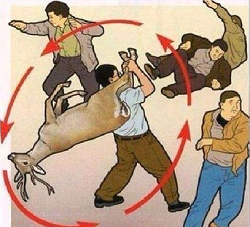
\includegraphics[width=\figwidth]{pics/21/47.png}
	\end{center}
\end{wrapfigure}
Every man in the room, even the Mob Boss still balancing his stupid chair, stopped and stared in sympathetic horror as the unfortunate part-Ogryn swayed with every slight movement of the markswoman's hand. 
The tableau lasted a good ten seconds before Aimy delivered a final viscous twist and the giant goon toppled over like a slow-motion video of a tree falling… which gave Aimy just enough time to let out a panicked squeak as several hundred kilos of goon landed directly on top her.

The shocked pause continued, now punctuated by sobbing moans from the part-ogryn and muffled curses from underneath him, until something finally gave; 
specifically, the bolts holding the table's top to its base. 
Physics being physics, the slightly-bent metal tabletop flew off with enough force to, well, shear metal bolts. 
The good news for the chinless Mob Boss was that said force was in the opposite direction from him. 
The bad news for the two goons behind Sarge was that he still had all five augmetic digits firmly embedded in the table's surface, and was pivoting with every ounce of force and weight his beefy noncom frame could muster. 
The whirring square of metal wasn't razor edged, but it still had more than enough sheer mass to crumple the chest of the goon who didn't duck in time, and seriously concuss the one who nearly did. 


According to Sarge's vaguely-defined plan, the bloody tabletop of justice should've continued its arc and smashed into the Mob Boss right where his chin wasn't, literally decapitating the whole criminal organization in a single blow. 
Unfortunately tables aren't exactly known for being high precision weapons, and neither was Sarge for that matter. 
Outside, Doc, Tink, the trainees, and a score of assorted goons all flinched as the shed's door blew off its hinges and a ballistic table wobbled overhead like a badly thrown frisbee. 
There was a pause, followed by a screech of "Waste 'em!" and the sound of someone panic-firing a silenced autopistol.

\begin{wrapfigure}{O}{\figwidth}
	\begin{center}
		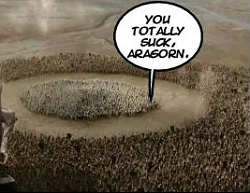
\includegraphics[width=\figwidth]{pics/21/48.png}
	\end{center}
\end{wrapfigure}
The ensuing brawl had two distinct parts. 
Outside, Doc and Tink jumped one of the two exterior door guards, while the ex-Cleric and Guardsman did for the other, but by the time both goons were down a perimeter had formed around the group, with the shed door in the no-man's-land in between. 


Things then stalled for a bit. 
On one side this was because Doc and Tink's group was outnumbered 4-to-1 (and that was counting the snoring Commissar mind you). 
On the other side it was because, well, they outnumbered Doc and Tink's group 4-to-1, so there was no reason why THEY had to be the first one to jump in and catch a wrench to the jaw. 
Far better to go second, or third, or maybe just stay at the back yelling "yeah" and "get them" until it was time to loot the corpses. 
This is, of course, why Sergeants were invented, but the goons seemed to be rather short on those, so the fight stalled out while everyone just stood there and listened to the shouts and thumps coming from the shed. 
Per long-standing narrative tradition, the standoff was broken by a thrown bottle.

Said bottle's contents were a matter of debate, which is to say: 
Twitch felt it should've contained 90% alcohol, a gelling agent, and a burning rag, while Nubby and the Trainees had argued in favor of something that wouldn't draw the attention of every Commissar in the camp, including the ones manning the inwards-facing heavy stubbers up on the walls. 
In the end, the demo-trooper had settled for a mix of the floor and drain cleaners he'd liberated from the laundry's supply closet, which didn't have quite the same effect as a proper molotov, but still left three men coughing and clawing at their eyes as Twitch and Nubby's group mounted their charge.

\begin{wrapfigure}{O}{\figwidth}
	\begin{center}
		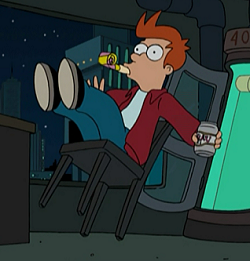
\includegraphics[width=\figwidth]{pics/21/49.png}
	\end{center}
\end{wrapfigure}
The inside portion of the brawl was, if possible, even less organized.

While Sarge's opener had done a number on the entrenching-tool armed goons behind him, it not only failed to remove the Mob Boss' autopistol from the equation, it hadn't even upset the man's balance. 
On the bright side, it's rather hard to simultaneously balance a chair on two legs, accurately fire a gun, and scream in terror as an enraged noncom throws himself towards you. 
This meant Sarge only took two of the four shots sent his way as he closed to melee range, and he managed to dodge two more through the masterful strategy of tripping over one of the concussed goon's feebly twitching legs and falling flat on his face. 
Sarge still managed to make a grab for the autopistol on his way down, and almost certainly would've snagged the weapon if the Mob Boss hadn't chosen that exact moment to finally teeter over backwards.

So on one side of the room there was Aimy still struggling to claw her way out from under the moaning Goon-gryn. 
On the other, one door guard was busy coughing blood while his companion stared vaguely around the room and tried to remember how his legs worked. 
So with both Sarge and the Mob Boss lying on the floor, that meant the only person in the room still standing was the Big Dumb Goon. 


Fortunately, the man lived up to his name, and didn't immediately sprint over and start stomping on Sarge's head. 
Instead he took a few seconds to cram the transfer orders in a pocket and grab one of the fallen entrenching tools, before slowly swaggering his way across the room while thumping the tool in his hand and doing the best evil-goon-laugh he could manage with a broken nose. 
He was rather surprised when Sarge decided not to just lie there waiting for his skull to be caved in, and grabbed the nearest available weapon: 
the Mob Boss' folding chair.

\begin{wrapfigure}{O}{\figwidth}
	\begin{center}
		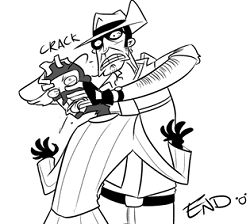
\includegraphics[width=\figwidth]{pics/21/50.png}
	\end{center}
\end{wrapfigure}
Once again, Sarge spun around in a blur of metal, blood, and simmering noncom rage, and where the Bloody Tabletop of Justice failed, the Equally-Bloody Folding Chair of Vengeance did the trick. 
The Big Dumb Goon blinked as the entrenching tool abruptly vanished from his hand along with most of the sensation in that arm. 
Next to him, the now re-concussed door guard flopped over in a boneless heap, and a little farther along the Chinless Mob Boss staggered to his feet and raised the autopistol just in time for the chair to sail under it, hit him square in the center of mass, and ragdoll him into the far wall.

The Mob Boss wasn't the first thing to hit the wall though, he was beaten there by Aimy thanks to a flailing Ogryn-sized boot to the backside right as the markswoman finally managed to claw her way out from under its owner. 
Aimy opened her eyes to find the room upside down and a ballistic Mob Boss bearing down on her, and immediately closed them again. 
When she re-opened them, the sight of a silenced autopistol pointed directly at her nose refocused her attention nicely, and after taking a second to see if the owner was going to pull the trigger, the markswoman lunged for the gun. 


At roughly the same moment as Aimy reached the autopistol, the Goon-gryn finished climbing to his feet, and no-longer blocked by his bulk, the room's rear door burst open to admit four legionnaires equipped with knives and entrenching tools. 
Aimy attempted some quick math involving the autopistol's clip size, the number of shots fired, and how many more goons were likely to be on the way, and then settled for pressing the gun against the limp Mob Boss' head and screaming at everyone to freeze. 
There was a tense silence, broken only by a sort of wet and crunchy sound from the man's neck-chin hybrid as the gun's barrel pushed his head over sideways. 
And then farther sideways, and farther, and farther… 

\begin{wrapfigure}{O}{\figwidth}
	\begin{center}
		\includegraphics[width=\figwidth]{pics/21/51.png}
	\end{center}
\end{wrapfigure}
Outside, the fight had stalled out again. 
The Mob Boss' shouted command and Twitch and Nubby's surprise attack had briefly escalated things, but without any real leadership present (on either side) everyone's self preservation instincts had taken over. 
The good news was that our little force had managed to steadily creep towards the door over the course of the brawl, and Doc was able to take a peek at the mess inside and relay the situation while the rest of us covered his back. 


Mind you, the angle of the door meant that Doc couldn't see the wall where Aimy and the Mob Boss had landed, or even as far as where Sarge was desperately trying to remain on his feet for that matter, so from the rest of our perspectives what followed was a bit confusing. 
First someone yelled "FREEZE", then someone else yelled "DEY WHACKED DA BOSS!", and then there'd been a long pause as everyone looked at the Big Dumb Goon. 
Doc described, for all present, a dawning expression of "uh, sort of like one of those little smashed faced bug eyed dogs slowly realizing it's been left unattended next to a steak dinner and trying to figure out what to do next." Further commentary was cut off as the Big Dumb Boss pointed a finger and began to yell something, only to be interrupted himself by an ear-ringing, window-rattling, parade-ground bellow of: 


>"COMMISSAR DOWN! 
PRISONER RIOT IN THE STORAGE SHEDS!" 

\begin{wrapfigure}{O}{\figwidth}
	\begin{center}
		\includegraphics[width=\figwidth]{pics/21/52.png}
	\end{center}
\end{wrapfigure}
Needless to say, Sarge's decision to call the entire bloody Commissariat down on us caught everyone by surprise, including Sarge. 
What exactly was SUPPOSED to have happened next was a mystery (which he later blamed on the fact that he'd been a bit busy and, you know, shot). 
What DID happen was that everyone present, with the exception of the abruptly awakened old Commissar, froze in place as the guards up on the walls started yelling to eachother and the spotlights mounted on their heavy stubbers began playing across the surrounding area. 
Then an alarm began to blare from the direction of the command building and the Big Dumb Boss screamed at his men to kill us and hide the bodies before the red-coats arrived while he handled the "Old Man", and then valiantly sprinted past his reinforcements and out the backdoor.

Doc relayed this all to the rest of the group, and by extension, all of the surrounding goons too. 
There were a few seconds of thoughtful silence, punctuated by the occasional meaty thump and silenced auto-pistol shot from inside, not to mention the distinct non-sound of nearly a third of the goons not-having-been-anywhere-near-there tonight sir, no, sir… And then the remaining two thirds charged.

Within a few seconds Twitch and two of the trainees were bleeding, Doc was being pulled up out of a muddy faceplant by another trainee, Nubby was casually sidling towards the crawl-space under the shed, and Tink had been viscously bottled in the back of the head by the Old Commissar.

\begin{wrapfigure}{O}{\figwidth}
	\begin{center}
		\includegraphics[width=\figwidth]{pics/21/53.png}
	\end{center}
\end{wrapfigure}
Inside, Sarge looked around fruitlessly for any more readily weaponizable furniture, and then swore and threw himself into a downright impressive dive for the fleeing Boss. 
His subsequent combat roll under three out of four wildly swinging entrenching tools and smashing through two pairs of legs would've been more impressive if the leg's hadn't belonged to Aimy's chair… The resulting confused half-chair half-noncom wrecking ball smashed into the wall next to the door and slid to the floor, where it alternated between bleeding, swearing, and trying to bludgeon the ankles of the four confused reinforcement goons.

Aimy missed all this, on account of the half-Ogryn trying to rip her head off. 
Well, more determinedly waddling towards her with his knees held tightly together, but there was no questioning the murderous rage in those piggy little eyes. 
So the markswoman dropped the Mob Boss' corpse, took aim, and placed an autopistol round directly into the half-Ogryn's forehead. 
Her expression when the bullet bounced off with a little hollow bonk and weee-owwww sound would've been amusing if anyone had the attention to spare.

In panicked reflex, Aimy flipped the fire selector to auto and tried again. 
Two of the six sub-sonic rounds wound up in the ceiling, one hit the dead mob-boss, and the remaining three just stopped, firmly embedded in the half-Ogryn's forehead as the big guy kept coming. 
There was another moment of panic as Aimy realized she had somewhere between 1 and 3 bullets left, and (if she crawled fast) about 10 seconds in which to use them. 
Fortunately the Markswoman's training kicked in before she ran out of either, and she belatedly shifted her aim downwards. 
The half-Ogryn's eyes widened and he clapped both his hands over his groin, only to keel over to the side as Aimy shot out his left knee with her last two bullets instead. 
She then swore as the big bastard just started crawling towards her.

\begin{wrapfigure}{O}{\figwidth}
	\begin{center}
		\includegraphics[width=\figwidth]{pics/21/54.png}
	\end{center}
\end{wrapfigure}
In the middle of this chaotic little melee, math was happening. 
Well, not "math" per se, Tink had a bit of a concussion, so it was more vaguely-math-shaped blobs slowly drifting across his brain like fuzzy little clouds as he desperately tried to stay upright. 
It involved X Goons, Y Guardsmen, and Z seconds until the Commissariat arrived, and Z was worryingly large. 
He vaguely looked around, registering an entire drop-shuttle's worth of of Real Bad Shit, and the considerably-less-than-Z seconds left before it really started Going Down. 


Tink's gaze finally landed back on the old Commissar, indiscriminately menacing everyone nearby with the jagged remains of the bottle he'd just broken over Tink's head. 
In a flash of inspiration, the techie pulled out the Commissar's dataslate, ducked under the wildly swinging bottle, grabbed the man's "non-drinkin" hand, and jammed the greasy, sausage-fingered paw down onto the dataslate's Big Red Button. 
He then flopped to the ground, flailing around like a fish, as his Penal Legion Discipline collar replaced his nervous system with white-hot razor wire.

Whatever the Big Dumb Boss had done to slow down the arrival of the Commissariat must have worked, because it was a solid (and very unpleasant) two more minutes before the relief force finally arrived, and found Aimy and the Old Commissar surrounded by spasticly-twitching Legionaires.

\begin{wrapfigure}{O}{\figwidth}
	\begin{center}
		\includegraphics[width=\figwidth]{pics/21/55.png}
	\end{center}
\end{wrapfigure}
The pointy-hats arrived in two distinct groups. 
The first one consisted of the old sour-faced bastard, backed up by his entire retinue of Cadets, and with the Big Dumb Boss nervously lurking right behind him, you know, just to make things obvious. 
 Or he was lurking, until he crossed the invisible 50-meter radius around our Commissar's dataslate and abruptly flopped over into the mud like the rest of us. 
Sour-Face actually stopped for him, or at least to give him a few kicks, before grumpily taking out his own dataslate and tapping in an override command. 
We all enjoyed a brief second of blessed relief, and then the collars reactivated as the drunk old bastard mashed his thumb back down on the panic button while stubbornly glaring at his counterpart.

Nobody except Aimy was in any condition to appreciate the ensuing pissing match. 
She described it as "a struggle of wills worthy of story and fucking song" and gleefully recounted Sour-Face's expression when he finally stomped across the field to wrest the dataslate away… just in time for the second group of Commissars to arrive and ask what in the Emperor's name he was doing. 


The second Commissariat relief force was led by our two depressed Cadets, who had the familiar look of people desperately hoping that whatever was going on wasn't their fault. 
Rather more importantly, it was also commanded by the Commandant, who, since Aimy had apparently scheduled our meeting during some big distracting brass-brief, had brought along a nice big audience of senior officers for the good ol' public reaming that followed.

\begin{wrapfigure}{O}{\figwidth}
	\begin{center}
		\includegraphics[width=\figwidth]{pics/21/56.png}
	\end{center}
\end{wrapfigure}
Now, it didn't start as a reaming: 
getting caught mid-slapfight with another Commissar might've been a bit undignified, but was perfectly understandable to anyone who'd actually met our Commissar. 
The point where the "discussion" escalated happened pretty quickly though, roughly five choked seconds after Aimy identified herself as "Cadet Von-Humpeding" to be exact; 
she didn't even get a chance to start lying about what happened. 
The expression on the Commandant's face just sort of congealed, and then started reddening as he looked between Aimy and the grumpy old Commissar, until he finally exploded into full-on screaming rage.

Like all properly epic reamings, this one had evidently been building up for a good long while. 
The gist was that Sour-Face did NOT run this camp and the Commandant was well and truly done with his "bullshit little power games", but the fine details went on at length. 
Once or twice the old bastard tried to interrupt with stuff about this being the right time and place, but the Commandant wasn't having ANY of that, and just kept on going, all while our drunk old Commissar watched on with sort of vindictive glee. 
The rest of us were more focused on getting our shit together now that the collars were finally turned off, and figuring out how to talk our way out of this when the Commandant got around to asking questions.

For like the sixteenth time, our asses were saved by our former trainees. 
The ex-scribe and cleric had been thinking down exactly the same lines as Tink, but had the forethought to actually put on their scan-proof scarf-thingies first. 
Then when Tink beat them to the punch, they'd then been smart enough not to walk around and get noticed. 
Now they were up on their feet, helping Aimy collect everyone and providing someone who was NOT Sarge to handle the talking.

\begin{wrapfigure}{O}{\figwidth}
	\begin{center}
		\includegraphics[width=\figwidth]{pics/21/57.png}
	\end{center}
\end{wrapfigure}
Our Drunk Old Commissar's attention was seized via a dose of stimm and the offer of a fresh bottle. 
We got his gaze focussed on the general vicinity of Aimy, who was actually TRYING to look like a grateful rescue-ee, and then a very edited version of the last several minutes was "remembered" to him. 
We weren't sure how much really sank in, but the idea that he might have done something heroic definitely seemed to have been established, and he seemed nearly coherent by the time the ex-Cleric unsubtly asked how much it would annoy Sourface if Aimy were to become one of HIS Cadets. 


Eventually, the raging Commandant brought us all back to "THE PRESENT SERIES OF TOTALLY FORESEEABLE, EASILY PREVENTABLE, COMPLETELY SELF-INFLICTED FRACK-UPS." On cue, Aimy stepped forward again to give her report, and then surprised the shit out of us with this sudden spiel of High Gothic in this weird sort of bossy nasal drawling accent. 
It honestly sounded nothing like her, well, not the bossy part, more the baked-in tone of aristocratic arrogance... 
that and the lack of profanity. 


In any case, whatever Aimy had just said, at least half of the commissars present understood it, judging by the expression of dawning horror as they all looked from her to our nearly-coherent Commissar. 
To our amazement, the man actually SAT UP, and then slurred… something. 
In the best traditions of overly-competent subordinates and evil royal advisers, the Cleric translated an acceptance of Aimy's "life debt", as well as a request that the Commandant allow him to take over her training. 
The Commandant just stared, his eyes bugging out slightly and mouth hanging open, until the old Commissar broke the silence.

>"Caush she's got nishe tits!" 

Aimy maintained her pokerface, and nodded in agreement with this sage wisdom.

\begin{wrapfigure}{O}{\figwidth}
	\begin{center}
		\includegraphics[width=\figwidth]{pics/21/58.png}
	\end{center}
\end{wrapfigure}
While everyone else in the audience (the word definitely qualified at this point) tried to figure out what to say after THAT, Commissar Sour-face smugly pointed out that the old drunk already had his maximum of two Cadets. 
The Commandant, visibly relieved to have something else to occupy his attention, rounded on the man with a bellow of "YES, TWO, NOT TWELVE! 
TELL ME, CAN YOU COUNT TO TWELVE!? 
LET'S PRACTICE ON THOSE CADETS BEHIND YOU! 
1! 
2! 
3!"

Before the reaming could really get going again, we gave our Commissar a firm poke. 
The man abruptly interrupted the raging Commandant, and in something very near to complete sentences, announced that his current pupils were doing so well that they were ready to return to regular training rotation. 
The appallingly hopeful expressions that suddenly seized the two Cadets' faces was something to see, as was the Commandant's when Sour-face interrupted yet again.

Showing an absolute inability to take a hint, the vindictive bastard snidely pointed out that our Commissar didn't even know what his Cadets looked like, much less whether they were fit for duty. 
This time the Commandant actually paused to consider the inarguably valid point, which gave the two Cadets time to solve the problem by running over to their chair-bound superior and desperately saluting him. 
Our Commissar surveyed the sweating pair with vindictive glee, and then jabbed a finger at one of them-

"Yeah, dish one here, havint caught im with any more porno-slates of Felinid guardswomen since-"

The Commandant cleared his throat and asked if he meant Cadet Yuriev, and was informed that "I calls im Yiffy, cause the porno-slates of the-" before the blushing Cadet in question loudly thanked his superior for his support, and ran for the barracks. 
The other Cadet, an expression of desperate optimism on his face, pointed out that the Commissar had said BOTH of them were ready, and got shot down with a "Shaddup Sniffy".

\begin{wrapfigure}{O}{\figwidth}
	\begin{center}
		\includegraphics[width=\figwidth]{pics/21/59.png}
	\end{center}
\end{wrapfigure}
After a few seconds of croggled silence, the Commandant just nodded at Aimy, and then we seized our chance and made a tactical withdrawal under cover of Sour-face's attempt to snap-graduate eleven of his Cadets into full Commissars, and the Commandant's enraged response. 
A miserable-looking Cadet "Sniffy" started to come with us, but Aimy's cheerful (yes CHEERFUL) insistence that she wouldn't have any trouble taking care of the Commissar by herself cheered him up immensely and he buggered off. 
The old Commissar was also cheered by Aimy's declaration, and insisted she ride up on the pallet with him where he could "keep an eye on her". 
She handed him a fresh bottle instead, which he accepted as a decent substitute.

After a short detour to the medical tents to Commissarialy requisition some supplies, we returned to our barracks for our traditional post-battle "discuss what the hell just happened while Doc removes foreign objects from Sarge". 
Aimy was introduced to the trainees without any hair-related acrimony, the Commissar was tucked away into a corner with a fresh night-cap, and a round of drinks was brought out while we caught our prodigal markswoman up on events. 
For her part, Aimy didn't volunteer any details about her time in the Commissariat, and nobody aside from Nubby was dumb enough ask. 


\begin{wrapfigure}{O}{\figwidth}
	\begin{center}
		\includegraphics[width=\figwidth]{pics/21/60.png}
	\end{center}
\end{wrapfigure}
When Nubby had been retrieved from his defenestration, and Doc pronounced Sarge sufficiently patched up for both of them to grab a (single) drink, the subject of our upcoming infiltration was raised. 


With Aimy, everything seemed almost too easy. 
We no longer needed to worry about the time-limit on our collars, since she'd be able to go get a cadet dataslate first thing in the morning and bring it inside with us. 
We didn't need to worry about those stupid room codes that the Big Dumb Mob Boss had ran off with either, since she'd just be able to grab the Commissariat's copy of our transfer orders while she was there. 
Best of all, we now had a legitimate reason to go into the evidence storage facility: 
to go get her stuff. 


Overall, the day was declared to have been a resounding strategic success (a term Sarge flinched at), even if nobody, not even our former trainees, believed any of it had been intentional. 
Even the old Commissar was in high spirits, especially about Aimy bunking in our barracks, and repeatedly insisted on being wheeled back into the conversation to regale his new cadet with slurred ramblings about his glorious former career. 


Our good mood lasted until reveille, or to be more specific, thirty seconds after reveille was supposed to happen. 
The lack of several dozen vox units blaring the traditional distorted approximation of horns (played by equally distorted approximations of musicians), had Sarge sitting bolt upright and considerably more awake than their presence ever had. 
After patiently waiting an entire minute to see if it was just late, he bawled the rest of us upright, and a reconnaissance expedition was launched.

\begin{wrapfigure}{O}{\figwidth}
	\begin{center}
		\includegraphics[width=\figwidth]{pics/21/61.png}
	\end{center}
\end{wrapfigure}
The camp was quiet, primarily populated by the few other life-long soldiers in the legion nervously whispering to each other about the unexpected break in routine. 
There was a small crowd gathering at the mess tent, but aside from that the only visible activity was around the command building and commissars' barracks. 
On closer inspection this activity seemed to involve a lot of boxes being taken out to the shuttlepad, and the realization of the only likely explanation hit us all at once: 
the Penal Legion was being deployed.

Aimy was immediately sent in along with the still-snoring Commissar (for moral support), and returned a short time later with Cadet Sniffy in tow. 
The morose cadet seemed to have reached a whole new level of despair, and mostly just whined about how everyone except him, Aimy, and the two old Commissars would be moving out. 
Aimy and the trainees tried to prod him for more details, specifically details about the daily details and if they'd still be happening. 
They weren't having much luck until Sarge stepped forward, pulled the Commissar's dataslate out of his chair, and handed it to the ex-Scribe with directions to just transfer the little turd. 
Sniffy sniffed, and pointed out that he wasn't an idiot and had tried that on his first day: 
the Commissar's dataslate didn't have permissions to do anything more than a cadet's, for obvious reasons.

Still though, this show of good faith won some grudging cooperation from the Cadet. 
His remaining reluctance evaporated completely when Sarge and the ex-PDF trooper pulled the young man aside, and pointed out that Aimy wasn't the sort of noble scion to forget a favor, and neither was her mother. 
A decidedly un-subtle hint that if Sniffy helped us with our little "laundry run" he might get his longed for transfer sooner, perhaps even today, was enough to win him over completely.

\begin{wrapfigure}{O}{\figwidth}
	\begin{center}
		\includegraphics[width=\figwidth]{pics/21/62.png}
	\end{center}
\end{wrapfigure}
With the downright eager assistance of Cadet Sniffy it was established that there wasn't an official schedule for work details, since the embarkation would be starting that afternoon. 
Fortunately, there wasn't anything scheduled at all until then, so if we cleared it with the perimeter commander, we could presumably go whenever we wanted. 
He wasn't exactly clear why Aimy, or the rest of us, wanted to go do laundry so bad, but he definitely wasn't someone to look a potential gift-horse in the mouth. 
Aimy requisitioned him as combination guide and Commissar-pallet-pusher, and went off to get approval, a dataslate, our transfer orders, and "a damn gun".

By the time Aimy returned, sans Sniffy, the camp was in a quiet uproar as the rumor of imminent deployment spread like wildfire. 
Under-occupied legionnaires milled around speculating about what sort of meat-grinder awaited them, and trading gossip about the death of the mob boss and Commissar Sour-face's very public fall from grace the previous night. 
Under the cover of all this, nobody even noticed us until our whole group had made it to the main gate, where a distracted pair of cadets waved us through without even checking Aimy's proffered dataslate.

Once in the laundry building, preparations began in earnest. 
Doc and most of the trainees went to do a quick scout of the freight bay to make sure we could still use it as our exit, and to cadge the name of the next shift's commander if possible. 
The Commissar, napping peacefully thanks to a pre-emptive sedative from Doc's limited supply, was parked in the corner with Tink, who was prepping a laundry cart with our uniforms and supplies. 
While the ex-Scribe briefed Aimy on the front-door security procedures she'd be talking us through, the rest of us did a load of laundry.

Or at least we started to do a load, until our collars all suddenly activated at max power and someone kicked in the door.

\begin{wrapfigure}{O}{\figwidth}
	\begin{center}
		\includegraphics[width=\figwidth]{pics/21/63.png}
	\end{center}
\end{wrapfigure}
Commissar Sour-Face practically radiated smugness as he strode into the room, one hand holding his dataslate while the other kept his bolt-pistol trained on Aimy. 
He was alone for a change, not that it seemed to bother him as he snidely reminded Aimy that Rule Number Three was "no weapons'' and gestured at her to disarm. 
For her part, the markswoman stood stock-still, glaring at the man with more hatred than any of us had ever seen before, not that we were in any condition to see it right then either.

After several seconds of futile stalling, Aimy grudgingly parted with her newly-acquired laspistol and chainsword, earning her a rage-inducing "good girl" from the smug Commissar. 
Her dataslate came next, though it was already showing an "unauthorized user" message on its screen, and the whole lot was kicked out the door, which was kicked shut in turn. 
Surprisingly, he then holsted the pistol, swapping it for his damn dataslate and gloatingly holding his finger over the "execute" button as he surveyed the room full of twitching guardsmen. 
He snidely reminded Aimy that there was a reason the regulations forbade "fraternizing" with the rabble, not that he believed that's what we actually were. 
Then, to our collective amazement, the man started monologuing.

It quickly became apparent that Sour-face wasn't any more hinged than our Commissar, at least judging by his rant about how Aimy was going to be his ticket out of there, one way or another. 
And we were in position to judge, because inside the laundry hamper Tink had fallen into when his collar activated, the techie had finally managed to wrangle the anti-scan bag around his collar. 
It was sheer luck more than anything else that he wasn't spotted as he poked his head up to survey the situation, and even luckier that the exact two tools he needed were right there next to him.

\begin{wrapfigure}{O}{\figwidth}
	\begin{center}
		\includegraphics[width=\figwidth]{pics/21/64.png}
	\end{center}
\end{wrapfigure}
While Aimy desperately kept herself still and the Commissar ranted about not-so-former Inquisitorial agents thinking they were smarter than him, Tink grabbed our Commissar's dataslate, carefully set it for the lowest shock setting, and overrode the previous command. 
Down on the floor, we all gained a newfound appreciation for that lowest collar setting, and did our best to catch our breath without blowing our cover, while Tink dug out the silenced autopistol we'd appropriated last night and took careful aim.

The Commissar was too wrapped up ranting at Aimy about how he'd beaten the Inquisition at their own game to notice anything until the autopistol hit him in the forehead. 
As in literally, with a little metallic bonk, because we hadn't managed to grab any ammo for the damn thing... 
Honestly, it was a mystery why we'd even brought it. 
In any case, even if Tink didn't have the same sort of lethal throwing arm as Sarge (and had actually been aiming for the dataslate in the Commissar's hand), the pistol's impact butt-first into the man's forehead gave us the opening we needed. 


Actually, the impact itself barely even fazed the Commissar, it was the second or so of confusion as he brought up the dataslate and fruitlessly tried to find Tink's collar on its display that gave Aimy enough time to lunge for the man's neck. 
Not that Aimy's attack went any better than Tink's; 
the crazy old Commissar was fast, far faster than someone his age had any right to be in our opinions. 
Aimy's lunge abruptly changed direction as the man spun out of the way, grabbed one of her reaching arms, and threw her across the room accompanied by the audible pop of a dislocating shoulder-joint. 
However, this in turn gave Twitch enough time to act, and one of his home-made chem grenades smashed against the Commissar's chest.

\begin{wrapfigure}{O}{\figwidth}
	\begin{center}
		\includegraphics[width=\figwidth]{pics/21/65.png}
	\end{center}
\end{wrapfigure}
Amazingly, even getting doused in whatever cocktail Twitch put in those things wasn't enough to do more than slow the crazy old bastard. 
The Commissar reeled backwards, holding his breath and keeping his eyes closed until he was clear, and then abruptly turned and put his boot into the ex-Scribe's face mid-tackle. 
Nubby's own lunge fared a bit better thanks to his shock-proof augmetics, carrying him over the face-planted trainee and directly towards the Commissar's face, only for the man to snatch him by the collar mid-air, and hurl the little trooper across the room. 
It was when he realized that Nubby was holding his precious dataslate that the man started to panic.

The Commissar immediately reached for both his pistol and chainsword, but didn't manage to draw either before Sarge's shoulder-check hit him in much the same way a Flyrant hits a dumb Scout Marine. 
The impact as the pair hit the industrial-scale laundry units was quite literally bone-shattering, and while Sarge managed to stagger upright on his third attempt, the crazy old bastard stayed down for the count.

By the time Doc's group returned a convenient minute later, we'd retrieved everyone from their assorted hard landings, disarmed the apparently unconscious Commissar, and opened some windows before we all choked on weaponized cleaning agents. 
Our medic was not exactly thrilled to find himself dealing with yet another round of collar-burns, not to mention the ex-Scribes badly broken nose, Aimy's dislocated shoulder, and Sarge's self-inflicted concussion. 
On the bright side, the scouting mission had gone fine, and our acquisition of Commissar Sour-face's unrestricted control dataslate opened up some interesting opportunities, assuming Tink could get it to work for him that is.

\begin{wrapfigure}{O}{\figwidth}
	\begin{center}
		\includegraphics[width=\figwidth]{pics/21/66.png}
	\end{center}
\end{wrapfigure}
The Commissar's dataslate had locked itself the second it left his hands, and was now demanding both a biometric authorization and access code. 
Per usual, Tink claimed this was easy to bypass, or would have been if he had all his stuff, but lacking those he'd just see what he could do with our Commissar's slate and a screwdriver. 
After several minutes of poking at the thing and ignoring helpful suggestions from Twitch and Nubby, he informed us we had a choice. 
The techie was fairly sure that he could get around the access code by restarting the dataslate, leaving just the biometric lock, problem was the dataslate was still broadcasting its normal signal to our collars, and restarting would disable that. 
If he was wrong we'd lose the signal, and since Aimy's dataslate was completely disabled, that'd leave us short...

Sarge, Doc, and Twitch all listened to Tink's explanation and pondered the problem, while Aimy flexed her re-located arm, and stalked off to retrieve her gear. 
After several seconds, Sarge broke up the discussion, and asked Tink just how sure "pretty sure" was, and whether anyone had checked if the slate's biometric lock was one of the fancy ones that could tell if the user was conscious or not. 
In the background, there was the high pitched whine of a chainsword activating, followed by a short terrified scream, and then the sort of grisly rending sounds and screaming typically associated with Khornate Space Marines. 


Twitch told everyone that he'd known the guy was faking being unconscious, and Tink suggested that it would probably be better just to leave the slate on.

\begin{wrapfigure}{O}{\figwidth}
	\begin{center}
		\includegraphics[width=\figwidth]{pics/21/67.png}
	\end{center}
\end{wrapfigure}
Nubby was dispatched to find a mop while the rest of us got back to work on the mission prep and laundry, and Sarge did a mental wellness check on our hyperventilating markswoman. 
Which is to say, he asked Aimy if she was feeling better, got a "Yes", asked if she wanted to talk about it, got a "No", and then shrugged and yelled at her to clean her uniform. 
Aimy blushed.

Once the load was done, our laundry hamper was prepped, and the Commissar's remains had been scraped into a laundry hamper of its own, Sarge gave the order to move out. 
The trainees went off to the freight entrance with the bin full of fresh-diced-Commissar and the man's dataslate, with directions to keep our exit open and make sure nothing important got accidentally incinerated mid-mission. 
The rest of us, still wearing our Penal Legion uniforms except for Aimy, formed up around our laundry trolley and the Commissar's pallet, and went right in the front door.

The lobby of the Mundane Evidence Storage Building wasn't particularly impressive, consisting primarily of a drab little carpeted room with a few uncomfortable chairs and a recaff machine that had last been cleaned sometime during the Horus Heresy. 
The security checkpoint immediately past it was rather more impressive, what with all automated gun emplacements and cybermastiff kennels lining the airlock-esque scan room leading into the building proper. 
The terminally bored Inquisitorial Stormtroopers manning the checkpoint were equally impressive, at least until they registered our decidedly non-Inquisitorial appearances, and brought out the recaff mugs they'd stashed out of sight when the door opened.

Rather than wait to be asked what in the Emperor's name we thought we were doing there, we rolled the cavalcade past the door sentries and into the scan room, where Aimy stepped forward and announced that she was there to "Get her shit". 


\begin{wrapfigure}{O}{\figwidth}
	\begin{center}
		\includegraphics[width=\figwidth]{pics/21/68.png}
	\end{center}
\end{wrapfigure}
The Stormtrooper Sergeant manning the little desk just inside the scan room eyeballed our spokeswoman in appropriately sergeanty fashion, but dropped the act when she added "And deliver some laundry". 
The sight of a bin of freshly cleaned uniforms, topped with a massive heap of still-warm socks and underwear, caught the immediate attention of every Stormtrooper present like, well, a load of clean socks. 
It's a soldier thing.

Unfortunately for the grunts on duty, Aimy wasn't willing to part with her laundry-bribe, at least not without a signed receipt, specifically from the next shift's CO. 
These being orders from her vaunted superior (currently snoring on the pallet), Aimy wasn't willing to budge on the issue, leaving the Stormtrooper Sergeant trapped between two equally valid maxims about letting sleeping Commissars/Officers lie. 
On cue, Sarge suggested leaving the laundry-bribe somewhere secure (see: 
the nearest security breakroom) while Aimy's other request was dealt with, and a signature could be obtained on the way out. 


Sarge's pointed interjection earned him some eyeballing of his own, but for once his Diplomacy training paid off. 
A simple grunt of "Ex-Stormtrooper", a gesture at all of us with a second grunt of "Unit", and a final grunt of "bullshit Inquisitorial power politics" was enough to elevate our collective status from "scum" to "poor bastards". 
Aimy's own assurance that she was only wearing "this dumb fucking hat" because of politcal bullshit bore fruit as well, especially when she more formally requested entry to pick up the personal effects of one Amelia von Humpeding before we all got deployed in a few hours.

\begin{wrapfigure}{O}{\figwidth}
	\begin{center}
		\includegraphics[width=\figwidth]{pics/21/69.png}
	\end{center}
\end{wrapfigure}
Interestingly, all the goodwill our blatant bribery earned us was overshadowed by the Stormtroopers' response on hearing Aimy's name. 
The Sergeant did a double-take, and then buzzed someone on his desk's vox unit, before abruptly getting up and leaving through the door behind his desk. 
The two Stormtroopers on door duty just shrugged when we looked at them.

After a short wait, during which Nubby managed to exchange a few pairs of socks for a round of hot drinks, the Sergeant returned accompanied by something so surprising that lesser men would've spat their recaff: 
a Stormtrooper Rupert. 
Not THE Rupert of course, rather the exact sort of painfully keen and woefully inexperienced junior officer that'd doomed more honest guardsmen than all the Traitor Marine legions combined, but in a Stormtrooper uniform. 
We all stared in shock, I mean, logically we knew that Stormtroopers had junior officers just like everyone else, but we'd always assumed they just started at Captain or something. 
Seeing a Stormtrooper with LT tabs was just wrong, and the experience was not helped by the way he boggled at Aimy like a recruit that'd just been issued his first porno slate.

After a small prod from his Sergeant, the Stomtrooper Lieutenant stepped forward, and ascertained that Aimy was indeed here for her stuff, and yes it was urgent, because we were all deploying, and yes Aimy was really one of THOSE Von Humpedings. 
The obvious firmly stated, the LT retreated through the door along with the rather put-upon Sergeant, only to reappear at the room's observation window and press his face up against the decidedly two-way glass. 
Nubby and Tink snickered as a large foggy patch grew around the Storm-Rupert's face, but fell silent when Aimy reminded them who here had a chainsword.

\begin{wrapfigure}{O}{\figwidth}
	\begin{center}
		\includegraphics[width=\figwidth]{pics/21/70.png}
	\end{center}
\end{wrapfigure}
After several awkward minutes, the LT disappeared from the window and the Stormtrooper Sergeant returned. 
While a dozen servo-skulls emerged from the wall ports and flitted around, presumably doing scanny stuff, the Stormtrooper Sergeant quietly informed Aimy that there was a bit of a paperwork issue, but not to worry, because they'd gotten her "The Good Scribe". 


Said Good Scribe turned out to be a wizened old man in an augmetic wheelchair, unfortunately accompanied by the Lieutenant. 
The jury was still out on whether the little tit was a ladder climber trying to score points with the family of a Lord General, or if he just had a thing for women in slightly blood stained Commissariat uniforms, but whatever the reason he was practically bending over backwards to make Aimy happy, and this included volunteering a squad of Stormtroopers to replace her retinue of Penal Legionnaires. 
On cue, Sarge volunteered to take our bin of laundry down to the guard room, along with the LT's orders, and before long a whole squad of neckerchief-sporting Stormtroopers returned, ready to escort and gofer the facility's honored guest. 
The question of whether the Lieutenant knew the appearance of his own men well enough to spot the swap was sidestepped when Aimy blithely responded to the facility's "no weapons" rule, by handing over her gore-covered chainsword, and asking the LT to personally take care of cleaning it for her.

With the Storm-Rupert out of the way, the Scribe assigned to us proved every bit as good as the Sergeant had promised. 
He waved away Aimy's sob story about her orders being mislaid, and the time critical nature of things given our imminent deployment to some horrible meat-grinder, assuring her it wouldn't be a problem at all. 
In a surprisingly short time, he'd managed to pull up the room number for her gear, produced and filled out a dozen or so arcane requisition forms, and led the way out to the final security checkpoint between us and the facility proper.

\begin{wrapfigure}{O}{\figwidth}
	\begin{center}
		\includegraphics[width=\figwidth]{pics/21/71.png}
	\end{center}
\end{wrapfigure}
This second checkpoint hadn't been on the Interrogator's plans, but that was understandable given it looked like it'd been set up within the last few days. 
It wasn't much, just a single Stormtrooper with a clipboard, and a senior looking scribe sitting at a desk covered with dormant servo-skulls. 
We watched as our scribe rolled forward and a sort of bureaucratic arm-wrestling match began, with a lot of arguing about the difference between a "release order" and a "disposal order", and why our request didn't violate some sort of "freeze". 


For his part, the Stormtrooper eyed us, and casually asked why we were all wearing scarves. 
There was a brief moment of panic, during which Sarge mentally ran through all of the vague excuses we'd come up with, before finally shrugging and just raising the edge of his scarf to expose the discipline collar, and announcing that we were wearing them because our Inquisitor was a massive asshole. 
The Stormtrooper winced in sympathy, but then frowned and pointed out that he only had authorization to let through active HQ troopers, and he would need to verify our credentials. 
Sarge began to proffer his doctored ID card, hoping like hell that Tink had done as good a job on them as he'd claimed, but the Stormtrooper waved him away and asked the pair of arguing scribes whether the psyker had come back from the bathroom yet.

\begin{wrapfigure}{O}{\figwidth}
	\begin{center}
		\includegraphics[width=\figwidth]{pics/21/72.png}
	\end{center}
\end{wrapfigure}
Fortunately, the answer to that question was "No", or more precisely, a sarcastic eye roll and a gesture at the general psyker-less-ness of the area. 
The Stormtrooper muttered something, and leaned over to the desk's intercom, and was rewarded with a pained voice telling him "Yeah yeah, but which massive asshole?"

To our collective relief Sarge actually managed not to blurt "Rogue Inquisitor Oak", but his decision to stand there silently panicking wasn't that much of an improvement. 
Fortunately, before any of us decided to try our hands at bullshitting past a psyker, our scribe helpfully suggested that if we could describe our Inquisitor, they could help us remember their name. 
Seizing the opportunity, all of us began rattling of a list of the most generic descriptors possible from "Paranoid bastard who doesn't tell his subordinates anything" to "Self-Important jackass who thinks everyone else is too stupid to breathe", and with a brief diversion into "tells your mom you got sent to a penal legion". 
All of these were accepted with the blank stares of people waiting for you to finish stating the obvious, until Nubby suggested "Big Stupid Hat?", and all three of them abruptly nodded, while the indisposed psyker swore at us for wasting his time and hung up. 
As the Stormtrooper waved us through the door, he suggested that next time we start with "The Inquisitor who's already here, doing the pre-trial inventory on the Oak case."

\begin{wrapfigure}{O}{\figwidth}
	\begin{center}
		\includegraphics[width=\figwidth]{pics/21/73.png}
	\end{center}
\end{wrapfigure}
As infiltrations of top-secret Inquisitorial facilities went, it was safe to say that we'd achieved the title of "Most Half-Assed". 
Honestly, we'd been grilled harder by stingy quartermasters, and Tau ones at that, but we weren't going to look a gift critter in the orifice, at least not without a good pair of gloves. 
That said, we did still try to pry some information out of the scribe as he and the servo-skull led us through the massive grid of corridors, but there was something about the place that seemed to discourage conversation. 
The walls just sort of drank in sound, making it hard to do more than nod along as the scribe nattered about how the recent servitor recall had made such a mess of things. 


In fact, according to the Scribe, the facility was so short on manpower they'd been trying to get the Penal Legion to assign a few details to help inside as well as outside, but they hadn't been able to get the security authorization. 
Doc broke in, and asked whether Aimy's assigned penal detachment could've come in with her under her security, and the rest of us groaned at the realization that we probably could've just walked in without any of the stupid disguise or laundry stuff. 
At least the helpful old Scribe was able to authorize the "return" of Aimy's legionnaires, actually printing out a little form from an augmetic in his chair, and handing it to Aimy with a cheerful suggestion that she just take it to the guards on the freight exit instead of bothering the main security office.

\begin{wrapfigure}{O}{\figwidth}
	\begin{center}
		\includegraphics[width=\figwidth]{pics/21/74.png}
	\end{center}
\end{wrapfigure}
The door our guide-skull led us to was a little smaller and lower security than most of the ones we'd seen, it was only the three Stormtroopers with a cargo pallet that set it apart. 
They seemed surprised to see us, boggling slightly at the sight of the snoring Commissar, but straightened up when the Scribe asked them what they were doing. 
After a short awkward pause, one of them explained that they had a disposal order for the room, and handed over a dataslate. 
The Scribe looked at it for a few seconds, announced he saw the problem, and promised to get it all sorted out. 
He instructed the trio to come with him, and began rolling off down the hallway, only to sheepishly roll back and open the door for us when Tink called after him. 


None of us had really known what to expect inside an Inquisitorial evidence store-room, but the reality was worse than we could have ever imagined. 
There were boxes, shelves, filing cabinets, and bins, all packed together more densely than any functionally sane human would want, but up above them was something terrible. 
Rows upon rows of metal racks reached all the way to the ceiling, every centimeter of them festooned with bulging opaque plastic wafers, each one containing a single vacuum-sealed item. 
Our entire arsenal (not to mention our tools, personal effects, several reams of parking tickets, and what looked to be several dozen empty beer bottles) had been clamshelled.

\begin{wrapfigure}{O}{\figwidth}
	\begin{center}
		\includegraphics[width=\figwidth]{pics/21/75.png}
	\end{center}
\end{wrapfigure}
The scribe handed Aimy a battered data wand, hastily explaining the litanies of identification and deactivation, and stressing the importance of not removing or breaking the seal on any item that hadn't been deactivated first. 
With a friendly direction towards the nearest supply closet, where cutting implements and first-aid kits could be found, he rolled off. 


Tink grabbed the wand, and hesitantly poked the little electronic seal on one of the corners. 
A hologram of a MRE appeared, along with a brief description, ID code, access log, and a little menu which Tink carefully navigated. 
The rest of us watched with growing impatience as the techie confirmed that he was sure he wanted to access the item, that he had read and understood the legal ramifications of accessing it, that he wanted to remove the item, that he'd read and understood the legal ramifications of removing it, and that he didn't want to review all those documents again.Twitch summed up the general mood with series of dire curses on all bureaucrats.

By the time Tink had the first few randomly selected items deactivated, and a pair of scissors had been fetched, broken, and abandoned in favor of Sarge's augmetic hand, it was obvious that this was going to take far longer than we had time for. 
Everyone but Tink (and the old Commissar, who'd been wedged under the racks at the far wall) began searching the racks and boxes for the real necessities. 
The room's small floorspace was ankle deep in vacuum sealed junk when Nubby, having climbed through the racks to the back of the room, triumphantly chucked out a distinctly lasgun shaped package. 
Not just any lasgun mind you, an oversized, blocky looking, totally-not-techno-heretical lasgun. 


\begin{wrapfigure}{O}{\figwidth}
	\begin{center}
		\includegraphics[width=\figwidth]{pics/21/76.png}
	\end{center}
\end{wrapfigure}
The realization that Oak had included our gear from the Occurrence Border boosted the mood massively, and Tink began excitedly badgering Nubby to try and find if Spot 3.0 had been included too. 
Sarge broke in to remind them guns, ammo, and combeads first, and informed the rest of us that there wasn't time for everyone to sit around here. 
He, Aimy, and Twitch would go off and scout for Oak's locker as soon as they were armed, and would return once it'd been located to get their collars off and plan the switch. 
Doc would stay behind with Nubby and Tink to supervise the search for Oak's boxes, and make sure the old Commissar didn't wake up and cause trouble.

As soon as Aimy had changed into our last Stormtrooper uniform, three weapons and the grenade Twitch insisted on having had all been extracted, and two combeads had been found, the scouting team set off. 
Tink immediately redirected Nubby to find his personal stuff first, ignoring Doc's objections, because everything would be SO much faster once he'd found his dataslate. 
Doc had barely even started grumpily going through the stacks of boxes when Tink extracted said slate, and triumphantly plugged it into the dataslate Aimy had left with him. 
Aimy's dataslate, now elevated to the full authority of a Commissar, not only supplied the IDs of Oak's boxes (which were in the far corner from where Doc had been searching), but finally unlocked those damn collars. 
The Medic, feeling relieved, but about as useful and appreciated as a Catachan Commissar, decided that was his cue to go do something more useful, and headed off with his Penal Legion Assistance Authorization Form to go get some more hands.

\begin{wrapfigure}{O}{\figwidth}
	\begin{center}
		\includegraphics[width=\figwidth]{pics/21/77.png}
	\end{center}
\end{wrapfigure}
With the annoying voice of reason out of the way, Tink and Nubby extracted the techie's plasma gun, and the unpackaging process became significantly faster, if rather foul smelling. 
Admittedly, this completely violated all those directions the Scribe had given us, but when the first one didn't trigger any alarms, Tink had declared it all a bunch of horseshit. 
It wasn't until a light started flashing above the door that it occurred to either of the pair to check whether the room had a fire detector, but fortunately it appeared to just be some sort of minor warning which quickly shut itself off as the room's air circulation automatically activated. 


Unfortunately the old Commissar was less forgiving, coughing and grumbling in a distinctly non-tranqed, not to mention exceedingly annoying, fashion. 
After the third outburst, Tink announced that enough was enough, especially now that we'd gotten out of the collars, and directed Nubby to dig the old geezer out and take him somewhere less distracting, like one of the servitor-storage rooms just down the corner. 
Nubby began to argue about being ordered around, but decided a little walkabout would be nice, anything to get him out of the cramped little fume-filled room faster really.

\begin{wrapfigure}{O}{\figwidth}
	\begin{center}
		\includegraphics[width=\figwidth]{pics/21/78.png}
	\end{center}
\end{wrapfigure}
A fair distance away, the scouting team was making some sort of progress. 
The duplicated ID cards were working to get them through the security doors at every junction, if a bit slower than things had been with the guide-skull, and there were enough other skull-less Stormtroopers walking around that they didn't really stand out. 
The problem was that while they had the ID number for Oak's room, which Sarge had "memorized" using a marker and his forearm, there wasn't any sort of directory, or even organization at all as far as Sarge and Aimy could tell. 
Twitch insisted there was a pattern though, one which he was on the edge of understanding, if they would just let him study the problem. 
Fully aware that Twitch had also said this about his breakfast cereal on multiple occasions, but lacking any better ideas, Sarge and Aimy fell into step behind the demo trooper.

Several minutes of back-and-forth semi-random wandering (and an awkward number of references to Sarge's forearm) later, Twitch led the trio to a junction door with a terminally bored Stormtrooper sitting in front of it. 
The Stormtrooper didn't look up from the dataslate he was holding as they approached, just boredly announcing that the junction's card readers were still broken, and they should just detour around it. 
Before anyone could stop him, Twitch triumphantly poked a finger at the man, accusing him of being One of Them. 
The Stormtrooper looked up in surprise, did a double-take at Sarge, and hastily shoved the slate into his pocket and came to a very embarrassed attention. 
Sarge shrugged in his best I've-got-other-shit-to-deal-with manner as the man muttered about "only watching it for the battle scenes" and dragged Twitch out before he could make things any weirder.

\begin{wrapfigure}{O}{\figwidth}
	\begin{center}
		\includegraphics[width=\figwidth]{pics/21/79.png}
	\end{center}
\end{wrapfigure}
At Twitch's insistence, the scout patrol continued around the grid to the other side of the junction, turning up two more terminally-bored Stormtroopers, before arriving at the final connected corridor, where a pair of far more professional-looking Stormtroopers blocked the way. 
Before anyone could think to stop him, the demo trooper walked up to the pair, and asked if Oak's shit was through there. 
He got a silent nod. 
Twitch asked if "Inquisitor Big Hat" was still there, and got a snort from the second trooper to go along with another silent nod. 
Twitch turned to Sarge and Aimy with a triumphant finger-guns, and raised the question of what to do next. 


Sarge turned, trying to avoid faceplate-contact with the two guards, while poking his combead in an attempt to raise Tink. 
After a few seconds of frustrating silence, he pulled the headset off, checked its indicators (which were all green), and started checking the other channels to see if he could hear anything on any of them. 
He stopped on the main Stormtrooper band, listening to the calming chatter of patrol check-ins, and then shrugged and announced that Tink's combead must be on the fritz. 
He began to suggest that we just get on with things as planned, when the door abruptly opened to reveal one of those incredibly creepy flying "cherub" sevitors. 
One of the guards announced that the Inquisitor was ready for us, and motioned for us to follow the creepy thing. 
Tink and Aimy stared in shock, but Sarge just nodded and motioned for the pair to follow him into the hallway.

\begin{wrapfigure}{O}{\figwidth}
	\begin{center}
		\includegraphics[width=\figwidth]{pics/21/80.png}
	\end{center}
\end{wrapfigure}
As it turned out, Oak's case did not have a room, it had the entire damn hall, both sides, and the "pre-trial inventory" was in full swing. 
The hall was littered with pallets, boxes, stormtroopers (of both the half-assed and rod-assed varieties), and at least a dozen scribes with data-wands and slates moving between the rooms. 
The only thing absent were the guide-skulls, having all been replaced by horrible flying cyber-babies with Inquisitorial icons stapled to them. 
Twitch quietly pointed out that anyone creepy enough to use Cherub servitors should automatically be considered a heretic; 
Aimy nodded in fervent agreement, and Sarge suggested that this really was not the time or place for that sort of discussion.

The cherub led them to the largest door in the hall, a void-shielded high-security job with wards all over it. 
In front of the door was a harassed looking man in a big dumb hat, waving a servitor control wand around and berating a random scribe. 
The Inquisitor (because there's no way he wasn't one) looked up in vague surprise as the group approached, and waved the scribe away. 
Sarge, lacking any better ideas, saluted and then stood there, while Twitch and Aimy silently watched and tried not to panic. 
The Inquisitor stared at Sarge for a second, and then waved his wand at the big door and ordered the three to follow him in.

Inside the room (more of a vault really) things were a lot less busy. 
There were a few elderly scribes off at a table on the side, along with a far younger scribe watching them. 
In the middle of the room, another young scribe as well as a pair of elderly Inquisitorial Savant types and a trio of Cherubs, fussed over a collection of clam-shelled items and three familiar-looking empty boxes. 
In the far corner, a final young scribe sat muttering into a large vox unit. 
Once the door was closed, the Inquisitor's demeanor immediately changed, and he gruffly demanded Sarge's report on what he'd found "in the Von Humpeding girl's vault".

\begin{wrapfigure}{O}{\figwidth}
	\begin{center}
		\includegraphics[width=\figwidth]{pics/21/81.png}
	\end{center}
\end{wrapfigure}
Back at said vault, Doc returned with penal-legion helpers in tow. 
The Stormtroopers working the freight bay had objected to him bringing in the trainees, but only because they'd been doing a great job of hauling stuff to the incinerator, and none of the troopers were keen on going back to doing it themselves. 
They'd bowed in the face of Doc's little printed form though, and reluctantly allowed their helpers to head inside, along with several empty pallets and one laundry hamper full of fresh-minced commissar.

Bringing the group through the facility hadn't been a particular problem either, except for the part right at the end, where Doc encountered Nubby trying to jam the sleeping old Commissar into the tiny supply closet across the hall. 
Doc sent the trainees in to start helping Tink, and went off to supervise Nubby's drunk-commissar-storage project. 
The cretinous little trooper whined that he'd checked every door he had access to, and the small supply closet was the only one even remotely acceptable. 
Doc pointed out that, even if Nubby did manage to fit the Commissar into it, the massive pile of office supplies he'd emptied out of it were a bit of a give-away, not to mention what would happen if anyone else needed to come get an easily-broken pair of scissors. 
Nubby insisted that the other rooms he checked were actually worse, for some unspecified reason, but grudgingly grabbed the Commissar's pallet, and followed Doc down the hall to re-check those servitor storage and maintenance rooms.

\begin{wrapfigure}{O}{\figwidth}
	\begin{center}
		\includegraphics[width=\figwidth]{pics/21/82.png}
	\end{center}
\end{wrapfigure}
A few minutes later, Tink looked up from where he'd been supervising the extraction of Oak's boxes, as Doc and Nubby returned and started shoveling freshly-opened weapons, explosives, and MREs into the Commissar's lap in an attempt to make space in the decidedly crowded little room. 
Tink was not happy with the return of this distraction, especially when Doc and Nubby couldn't really explain what was wrong with all the other rooms, just waving their hands and going on about how they'd checked and the rooms were "unacceptable". 
The trainees butted in, pointing out that having him there wasn't really that much of an inconvenience, especially now that the ventilation was on full blast, but the techie insisted that it would ruin his nice efficient process. 
Tink ordered the trainees to finish opening the items he'd already "deactivated" (he refused to leave his plasma gun with them, on the grounds that they'd probably break it) and then led Doc, Nubby, and the Commissar pallet out into the hallway.

The argument continued in the hallway for a minute, with both Nubby and Doc insisting that the only other remotely acceptable option was the little supply closet. 
Tink, agreeing about the stupidity of the little closet, but still trying to ascertain what exactly was so damn wrong with his previous drunk-Commissar-storage suggestions, finally yelled at Nubby and Doc to just show him, and grabbed the Commissar's pallet. 
A short walk brought the trio back to the door of the servitor storage bay, where Nubby rolled his eyes, jimmied the door, looked in, and then made a little "ah-ha!" gesture.

>"Daaaaaat was it! 
We couldn shove 'im 'ere cause its all full up wif nekkid dead guys!"

\begin{wrapfigure}{O}{\figwidth}
	\begin{center}
		\includegraphics[width=\figwidth]{pics/21/83.png}
	\end{center}
\end{wrapfigure}
Tink surveyed the room, with its tight rows of servitor-berths inexplicably filled with what looked like naked stormtroopers and a few scribes. 
After a few seconds of pondering, Tink pointed out there was still PLENTY of room if they just shoved 'em all up in a pile against the far wall. 
Doc explained that he'd already thought of that, and the problem was that only a few of them were actually dead. 
Wouldn't do to have them wake up and start asking questions about why people were shoving Commissars in there with them. 
Also, Nubby added, it would be super unhygienic and a lot of work. 
Tink nodded in reluctant agreement with their sound logic, and began to turn the pallet back around, only to abruptly stop part-way (nearly sliding its snoring cargo off) and ask what was wrong with the other room.

Doc and Nubby both looked at eachother, obviously waiting for the other to explain, until Nubby finally made a little apathetic shrugging gesture. 
He walked up the door labeled Servitor Maintenance and Control Shrine 4 and knocked on it. 
Tink watched, slightly nonplussed, as an annoyed-looking man in robes opened the door and firmly stated that NO means NO, not even if they asked pretty please or promised he wouldn't wake up, not to mention throw up! 
Doc immediately apologized and began offering tips on cleaning bodily fluids out of clothing, but stopped as the man made a little gesture and touched the glowing crystals on the orante necklace he wore.

Tink peeked behind the Psyker, surveying the impressive little cogitator array that had been wired into the building's main control and communication systems. 
He paused for a second, looking from the Cogitator, to the Psyker, to the closed Servitor Bay, and then back to Doc and Nubby.

\begin{wrapfigure}{O}{\figwidth}
	\begin{center}
		\includegraphics[width=\figwidth]{pics/21/84.png}
	\end{center}
\end{wrapfigure}
Tink took a deep breath, and pointed at the Servitor Bay.

>Okay, so we can't put the Commissar in that one because there's a bunch of stripped stormtroopers already hidden there.

Doc and Nubby both nodded, while the Psyker rolled his eyes and made a "get along with it" gesture.

>And we can't put him in this one because this guy is already using it for his secret Inquisitorial mission.

More nods and eye rolling.

>And that supply closet was way too small… unless I make it bigger that is!

Tink raised his plasma gun, and both Doc and Nubby nodded at this novel out-of-the-box solution. 
The psyker winced, and touched his crystals again, and all three guardsmen deflated as they realized that there were probably a lot of reasons why cutting holes in the wall with a xenotech plasma weapon was a bad idea. 
Tink paused, double-checking that incongruous thought, and then sighed.

>You know, if I had a throne for every time we blundered into another Inquisitorial team mid-mission, I'd only have two, which isn't a lot, but it's weird that it's happened twice.

Doc laughed. 
Nubby laughed. 
The Psyker blinked. 
Tink shot the Psyker.

Of course, now the problem was that, as Nubby put it, "Dere's dead psyker juice everywhere". 
Tink nodded in resigned agreement, admitting that it really wasn't the sort of place to linger in, you know, in case they caught dead-psyker-itus or something. 
Down on the floor, Doc finished putting a dressing on the definitely-dead Psyker's chest wound, and blinked a few times. 
As Tink and Nubby wheeled the Commissar out, Doc jogged after them, grabbed one of the pulse carbines off the pallet, and shot the psyker again, in the head this time, and then dragged the techie back in to take a look at the cogitator setup.

Nubby remained in the hallway with the Commissar, insisting he had a family history of dead-psyker-itus.

\begin{wrapfigure}{O}{\figwidth}
	\begin{center}
		\includegraphics[width=\figwidth]{pics/21/85.png}
	\end{center}
\end{wrapfigure}
In a room full of not-dead psykers, Sarge delivered an exceedingly precise report of the contents of Aimy's vault. 
To wit, parking tickets, guns, explosives, beer bottles, and more parking tickets. 
After nearly a minute of this, the Inquisitor held up a hand and clarified that he wanted to know what had happened and why Sarge was HERE.

Sarge winced at the feedback in his combead, both from the irate Inquisitor and the poorly-disguised psyker muttering in the corner, then reached up and turned the stupid thing off. 
Ignoring the Inquisitor's raised eyebrow, Sarge truthfully reported that Cadet Commissar Von Humpedig arrived to collect her stuff, and… they'd… uh… come here. 
Because orders. 
Aimy and Twitch shared a look of growing alarm, but the Inquisitor only sighed and asked Sarge why he wasn't wearing a psi-shield. 
The answer, "Because we weren't issued any?", did not seem to please the man. 
He glared at Sarge, which didn't really have much effect given the face plate. 


The inquisitorial glowering was interrupted by a shrill beep from under Sarge's scarf, prompting further demands as to why he was wearing a scarf, why said scarf was beeping, AND where his psi-shield was. 
Sarge, still standing at a firm attention, got as far as "Because…" before the Inquisitor held up a hand and declared that he really did not care. 
In an exasperated tone, depressingly familiar to us from our previous missions, he directed Sarge to turn around, go back to Aimy's vault, and STAY there until the Interrogator shows up, as had been outlined in the mission briefing. 
And then to go get a damned psi-shield.

Sarge, Aimy, and Tink, thanking the sweet merciful Emperor, saluted as the Inquisitor strode past them to reopen the door. 
Those thanks came to an abrupt halt as the door opened to reveal three familiar-looking stormtroopers, one of them with their hand raised to knock. 


\begin{wrapfigure}{O}{\figwidth}
	\begin{center}
		\includegraphics[width=\figwidth]{pics/21/86.png}
	\end{center}
\end{wrapfigure}
The Inquisitor figured out what had happened far more quickly than anyone else, which didn't really help him much, since Sarge, Twitch, and Aimy didn't waste any time at all on such silliness: 
they just opened fire. 
Two fully automatic pulse-carbines, and a double-tap from Aimy's rifle hit the Inquisitor… and then kept going as the man vanished with the distinctive crack of a Displacer Field. 
The three pseudo-Stormtroopers behind the man did not have displacer fields, or time to dodge for that matter.

Unfortunately, this abrupt opening didn't account for the dozen or two other Stomtroopers present, and even more unfortunately, the Inquisitor stuck his landing. 
A booming voice infused with psychic Will, ordered the three Guardsmen to drop their weapons. 
Sarge, along with half the Stormtroopers present, abruptly dropped their guns, as did Twitch, along with the grenade he'd just primed. 
A desperate kick caught the falling munition, propelling it off the far wall and out of sight down the hall, roughly in the direction which the Inquisitor's voice had come from. 
Aimy did not drop her weapon, because she'd already let go of it as she ran for the door's control panel, slamming the massive metal vault shut on a muffled *krump* and anguished "MY LEG!"

Sarge and Twitch recaptured their weapons from their slings, while Aimy mashed every single alarm and lock button on the panel, and asked Sarge just what the hell we were supposed to do now. 
Fortunately for the big, tired noncom the answer was obvious, because right about then the two Savants got over their shock and started screaming at their psykers to kill us.

\begin{wrapfigure}{O}{\figwidth}
	\begin{center}
		\includegraphics[width=\figwidth]{pics/21/87.png}
	\end{center}
\end{wrapfigure}
Actually, what the Savants were yelling was a bunch of gibberish "Throne-washes-Tallarns" stuff, but the intent was pretty clear as the three young scribes all sat bolt upright and turned to glare at us. 
The fact that they were psykers was also pretty clear, what with the nimbus of warpy energy forming around the one in the corner, and the one at the table levitating up into the air. 
The real clincher though was when the one over by the actual scribes abruptly turned into a daemonic horror the likes of which man was not meant to see; 
a towering flickering mass of mouths and all-seeing eyes, the sort of monstrosity that could not be fought, only fled in a futile attempt to postpone the inevitable grisy end. 
We shot it anyway though, because what else were we supposed to do?

Whatever the psyker thought was going to happen, it wasn't three guardsmen panic firing xenotech plasma weapons in an enclosed area. 
When Sarge and Twitch ran out of ammo all that was left of the psyker (not to mention the chair, table, half a shelving unit, and one of the hypnotized scribes' arms) was a smoldering stain on the vault floor. 
The two remaining psykers and their Savant handlers all stared in utter shock, which was finally broken as Aimy realized she still had a few shots left, and promptly shot one of the Savants. 
The remaining old man drew a needle-pistol and leapt for cover, screaming more command-phrases and gesturing with the data-wand in his free hand. 
Sarge and Twitch both ducked as all three cherub servitors swarmed them, prodding at their faces and hands with miniature shock-mauls while screeching and laughing in a far more disturbing way than the faux-Daemon had managed. 


\begin{wrapfigure}{O}{\figwidth}
	\begin{center}
		\includegraphics[width=\figwidth]{pics/21/88.png}
	\end{center}
\end{wrapfigure}
Sarge, cursing whatever had possessed him to come down here without his full kit, or at least a damn side-arm, tried to swat away the cherubs with his gun's butt while Twitch desperately tried to reload. 
He expanded that cursing to include his decision to leave the damn collar on, as the device in question suddenly progressed from beeps to "warning" shocks. 
Twitch added his own swears as his collar kicked in too and he dropped his reload. 


Realizing she was the only one with a functional weapon at present, Aimy fell back into cover and lined up a shot on one of the cherubs, only to miss entirely as an invisible force wrenched her pulse-rifle upwards. 
The markswoman, having just gotten her damn gun back and being none too keen on losing it again, tightened her grip on the bucking weapon. 
The telekine psyker grunted and pulled harder, until the pulse-rifle finally rose over the top of the shelves, with an irate Aimy dangling under it, loudly promising to shoot him in his stupid psyker face the second he let go. 


Sarge missed the magical levitating markswoman, at first because he was a little busy trying to fend off the cherubs, and then because his mind abruptly went blank. 
Across the room, the psyker by the vox unit let out a groan of distress as several decades of literally Guard-issue battle damage weighed down on his psyche, followed by a sharp electric shock to the neck. 
Sarge flinched and swore at his damn collar, and then blinked as he registered the (thankfully still empty) gun he had pointed at Twitch's head. 


Any introspection that might've happened after coming this close to fucking up was postponed as one of the cherubs whacked him right in the face-plate with its mini-maul. 
Sarge swore yet again, dropped his weapon onto its sling, and just grabbed the annoying little shit out of the air by a decoratively-flapping wing, and swung it into one of its companions in a spray of feathers and servitor-lubricant.

\begin{wrapfigure}{O}{\figwidth}
	\begin{center}
		\includegraphics[width=\figwidth]{pics/21/89.png}
	\end{center}
\end{wrapfigure}
Twitch, having finally succeeded in reloading, turned to take out the last cherub, only for his mind to go blank as well. 
Sarge, being gratifyingly quick on the uptake for a change, managed to grab the mind-puppeted demo trooper's weapon and yank the barrel upwards just in time. 
Twitch responded by repeatedly attempting to shank him with a sharpened fork, but didn't manage to penetrate the armor before his collar activated again and the psyker released him with a pained yelp.

A good three meters above all this, Aimy's deathgrip on her weapon carried her over the top of one of the shelving units, as well as the rather-surprised Savant using it as cover. 
Rather than wait for the elderly man to shoot her like so much skeet, the markswoman twisted her body around and planted both feet against the side of a heavy-looking box and kicked off as hard as she could. 
The box, proving even heavier than it looked, barely even shifted, the shelving unit on the other hand…

The Savant let out a little screech of terror and sprinted along the aisle, throwing himself to the ground as the shelves finally slammed into their neighbor, pushing it over as well and leaving him in a small gap full of falling clamshell casings. 
Aimy surveyed the carnage as a third set of shelves began to teeter, and found herself drifting off into a sort of peaceful doze. 
She didn't even realize she'd let go of her weapon until the strap caught her in the armpit, abruptly jerking her attention back to the present. 
Aimy twisted around to glare at the telepathic psyker by the vox unit, and after a brief survey of the available options, grabbed her stormtrooper helmet and hucked it at him.

\begin{wrapfigure}{O}{\figwidth}
	\begin{center}
		\includegraphics[width=\figwidth]{pics/21/90.png}
	\end{center}
\end{wrapfigure}
Twitch put down the remaining cherub just as soon as he'd convinced Sarge it was really him, and could he have his gun back now pretty please? 
He started to shift left down the aisle while Sarge reloaded his own weapon and moved right, and drew up to the end of the unit right as the badly-shaken Savant flung himself around the corner, ready to flank the two men his psyker and cherubs had tied down. 
Twitch made a sound somewhere between a scream and a yelp, and flinched backwards as bits of Savant-skull shrapnel pinged off his faceplate. 


At the other end of the aisle, Sarge ignored the weird sounds behind him as he spotted the glowing telepath psyker seated at the vox unit in the far corner of the room. 
His carefully-aimed shot missed as a ballistic helmet whacked the young man in the face, dropping him to the floor. 
Swearing some more, especially as the collar shocked him again, the noncom sprinted down the aisle, confirmed the kill, and turned to try and get a shot at the remaining psyker.

The telekine, a girl even younger than Fumbles (who insisted he was 23), abruptly realized that shit had gone truly south, and released a psychic shockwave that blew Sarge, Twitch, the Scribes, and several shelves backwards. 
Aimy was also hit by this blast, but true to her word, the second the markswoman's rifle was released from its psychic grip, she turned, drew a bead on the psyker mid-air, and dropped the girl with a solid center-of-mass shot. 
Having spared rather less attention for her landing, not to mention the psychic shockwave, Aimy swore as she bounced off two fallen shelving units, caught her leg on one of them, and found herself hanging upside-down staring at the terrified and confused Scribes. 
One of them raised their hand like a kid in school, and asked what was going on.

\begin{wrapfigure}{O}{\figwidth}
	\begin{center}
		\includegraphics[width=\figwidth]{pics/21/91.png}
	\end{center}
\end{wrapfigure}
In accordance with the laws of narrative causality, at precisely the moment when the Inquisitor had said "until the Interrogator shows up", a sallow-skinned young man and his two companions asked Nubby what he was doing standing in hallway with a pallet full of unconscious Commissars and odd-looking energy weapons. 
Corporal Nubby Nubbs, Inquisitorial Stormtrooper, saluted and proudly told the pale young man with the psyker-staff that he was keepin' watch while 'is mates Doc and Tink checked out da psyker closet. 
The Interrogator groaned, and motioned at one of his retainers to inspect the room.

Doc and Tink looked up from the cogitator unit as the door opened, framing a dark, lithe blur sprinting towards them. 
The medic reacted first, fumbling for his carbine, only for a hand to yank it out of his grasp and pull him forwards into what felt like a power-hammer blow to the chest. 
Tink got to watch as Doc got kicked past him with enough force to break his weapon strap, and then his own weapon was yanked forwards, dragging him out of his seat face-first into the plasma gun's butt. 
A slightly nasal feminine voice complained: 
"He got himself shot in the damn face by these idiots, and I think this one with the fancy gun might be a frakkin officer."

Doc and Tink tried. 
They really, really did. 
Despite the broken ribs, Doc managed to get back up and launch a tackle at the body-suited woman (who, to be fair, wasn't even looking at him), only for her to slap him in the face hard enough to shatter his faceplate and leave the stunned medic in a heap on the floor. 
Tink made a grab for his gun while she was busy, and got smashed in the face with its butt again for his trouble. 
Outside, the Interrogator casually reminded the woman not to kill anyone, while he focused on psychically examining Inquisitorial Stormtrooper Nubbs. 


\begin{wrapfigure}{O}{\figwidth}
	\begin{center}
		\includegraphics[width=\figwidth]{pics/21/92.png}
	\end{center}
\end{wrapfigure}
The Interrogator's other retainer, a tall lean man in a comically fancy coat and feathered hat, flipped up Nubby's visor to compare it against his security badge, and immediately regretted his decision. 
In a tone of horrified fascination, he pointed out that either the HQ Stormtroopers were really scraping the bottom of the barrel, or the Ordos Xenos had started doing diversity hires. 
The Interrogator frowned at this observation, while Nubby happily explained that he'd "never been to no 'versity", but was great at scraping things. 
The fancy aristo sneered and moved on to examining the snoring Commissar, companionably pointing out that at least the Interrogator didn't have to dirty his mind on that wreck of humanity. 
The Interrogator shuddered and shook his head as the short trooper excavated one of his nostrils, examined his findings, and ate them. 
After a brief disgusted pause, he told his minion to shut up and go check on the Von Humpeding vault.

The squad of penal-trainees didn't even look up as the door opened, being far too busy looking in literally any other direction. 
The aristo surveyed the scene for a few seconds, before closing the door again and asking whether anyone would miss a unit of penal legionnaires if they spontaneously disappeared. 
The Interrogator grunted in psychic effort and the man hurriedly closed the door again; 
after a few seconds of silent probing, he declared that the legionnaires had been officially approved by someone or other, so they'd have to disappear the records too. 
The two men began debating whether it would be easier to kill, incapacitate, or just mind-fog the legionnaires while they investigated the vault for anything Oak-related.

\begin{wrapfigure}{O}{\figwidth}
	\begin{center}
		\includegraphics[width=\figwidth]{pics/21/93.png}
	\end{center}
\end{wrapfigure}
In the dead-psyker-closet, Tink and Doc had decided staying down was the better part of valor, especially since the woman had finally gotten tired of re-breaking Tink's nose with the plasma gun, and was now holding it trained on the pair. 
Both guardsmen weighed their severely limited options, and lacking anything better, settled in to wait and see what happened next. 
That turned out to be the distant krump of a grenade, followed by several runes flashing red on the fancy cogitator setup. 
The woman stared in confusion at the mysterious blinking lights; 
Doc and Tink, having spent enough time poking at the thing to know that it was hooked up to the building's alarm system, decided the time had come for one last try.

Tink leapt at the woman, while Doc went for the cogitator. 
Realizing what was going on fairly quickly, she whipped the plasma gun towards Doc and pulled the trigger, and then stared in consternation as the gun emitted a short blue beam instead of a ball of plasma. 
Responding in the standard Imperial fashion for a warrior beset by unexpected weapon malfunctions, she raised her hand and gave the gun a good smack. 
Also responding in the standard Imperial fashion, the plasma-gun vented a blast of superheated gas directly into her face. 
Tink's tackle hit the woman roughly half a second later (his first successful hit of the fight), and while he didn't do more than stagger her, he did manage to get both hands on his beloved plasma gun. 
The blind leg-sweep she responded with hit his shins with considerably more force, as well with an unpleasant cracking sound.

Doc ignored the fight going on behind him in favor of desperately searching for the cogitor for some sort of "Approve" button. 
Deciding it either had to be the yellow check-mark or the green circle, he simply mashed both of them, and was rewarded with the sound of every vox in the building simultaneously blaring the fire, weapons-discharge, and emergency-lockdown alarms.

\begin{wrapfigure}{O}{\figwidth}
	\begin{center}
		\includegraphics[width=\figwidth]{pics/21/94.png}
	\end{center}
\end{wrapfigure}
Out in the hall, the distant grenade blast interrupted the Interrogator and his minion. 
Both men paused to listen as their combeads erupted into confused chatter, until this was interrupted in turn by the deafening blare of the facility's alarms. 
The Interrogator swore, tightening his mental control on the short stormtrooper and the room full of penal legionnaires. 
The elderly Commissar, not being under psychic compulsion or adequately tranqed anymore, jerked awake, looked around in vague confusion, and spotted a pale little tit with an inquisitorial rosette standing right next to the pallet with his eyes closed. 
With the malicious grin of someone who'd always wanted to do this, he hefted his empty bottle and smashed it into the man's skull.

Sadly, the Commissar didn't have quite the same level of strength as, say, Sarge, so the Interrogator didn't have his head caved in, but he did drop to the ground with a little yelp of pain. 
Needless to say, the Interrogator did not take this kindly. 
A concentrated blast of psychic pain left the old Commissar squealing and flailing in his chair, much to the surprise of the no-longer-mind-controlled Nubby next to him. 
With the honed survival instincts of a true cretin, Nubby responded to the complex tactical situation by screaming, kicking the downed Interrogator in the stomach, grabbing one of the weapons falling off the Commissar's lap, and diving for cover behind the man's chair. 


The aristocrat, viewing the whole situation with growing alarm, drew a comically small needle pistol, and asked his superior if he needed assistance. 
The interrogator instructed him to do something anatomically improbable, which he seemed to take as an order to start flanking Nubby's position.

\begin{wrapfigure}{O}{\figwidth}
	\begin{center}
		\includegraphics[width=\figwidth]{pics/21/95.png}
	\end{center}
\end{wrapfigure}
Neither Nubby or the Interrogator waited for the flanking maneuver. 
The Interrogator staggered to his feet, gesturing at Nubby in appropriately psyker-y fashion, only to screech in surprise as the little trooper lunged out of cover, brandishing a silenced autopistol. 
Abandoning his psychic attack, the man scrambled around the pallet barely ahead of a series of "bangs", desperately trying to keep the bulk of writhing Commissar between him and his assailant, and shouting warnings and instructions at the aristo. 
For his part, the dapper man picked his way through the detritus of half-packed crates, and pointed out that Nubby's gun hadn't actually been loaded. 
A slightly panicked voice from the far side of the Commissar informed him that it was totally, definitely, 100% loaded, and was just silenced. 
The aristo asked why he'd been shouting "bang" then, and was rewarded with the little trooper poking out his autopsistol, and yelling "fwip" instead. 
The Interrogator sighed in embarrassment, and made another, uninterrupted psychic gesture.

A short distance away, a very angry woman with plasma burns on her face stopped trying to dislodge the flailing, screaming Tink from the malfunctioning plasma gun, and just dropped both of them to the floor. 
Doc, knowing exactly what was coming next, scrambled away from the cogitator and tried to hide behind one of the servitor maintenance stations, only for a vice-like grip to close on his ankle and yank him out with enough force to fling the medic against the far wall. 
Her followup attack was interrupted as Tink switched the home-made fire-selector on his plasma gun from "cut" to "maximal", and shot her in the back.

\begin{wrapfigure}{O}{\figwidth}
	\begin{center}
		\includegraphics[width=\figwidth]{pics/21/96.png}
	\end{center}
\end{wrapfigure}
Amazingly, the woman actually managed to spin in place and PARRY Tink's shot. 
With her hand. 
While whatever mixture of augmetics, training, and magical bullshit that powered the woman's melee abilities was enough to deflect bullets, an overcharged ball of plasma capable of melting holes through tank armor was a bit of a tall order. 
Her hand didn't so much knock the plasma ball aside, as splash it, wreathing her whole arm in blue flame, scorching through her bodyglove, and reducing her hand to a fused, smoldering mass. 


Doc, seeing an opportunity but having no illusions about the woman's ability to beat his ass literally one handed, scrambled past the screaming, swearing, burning woman, and dove for the corner where his pulse carbine had landed at the start of the fight. 
Displaying far more tactical sense than usual for an inquisition agent, instead of chasing the medic, the woman started sprinting for the door. 
Tink, lying squarely in her path, brandished his plasma gun, realized it was obviously still recharging, and desperately tried to drag himself out of her way, barely dodging the kick the woman aimed at his head as she passed. 


Out in the hallway, Commissar Kelly swore as the ice-pick of psychic pain jammed into his brain pulsed with, upon reflection, not that much more discomfort than his more or less permanent hangover. 
It wasn't pleasant mind you, but really, it was a bit much to call it incapacitating. 
With an effort of will, the elderly Commissar brought his eyes and a decent portion of his mind into focus, and leaned forward to rummage in the pile of weapons in his lap. 
Next to his chair, the Interrogator grunted with effort as Nubby marched out of cover. 
The grimy little trooper handed the unloaded autopistol into the Interrogator's waiting hand, while the Commissar jammed his decidedly loaded laspitol into the Interrogator's waiting face.

\begin{wrapfigure}{O}{\figwidth}
	\begin{center}
		\includegraphics[width=\figwidth]{pics/21/97.png}
	\end{center}
\end{wrapfigure}
The aristocratic inquisitorial agent, having successfully navigated the battle without getting shot at, and very proud of that fact, screamed in surprise as his superior's head detonated in a spray of flaming skull fragments and meaty bits. 
There was a brief pause as the aristo took in the abruptly changed combat situation and a confused Nubby picked up the fallen autopistol and tried to jam it back into the corpse's nerveless hand. 
Then the Commissar spotted him.

The barrage of laspistol fire had more in the way of enthusiasm than accuracy, but it was enough to convince the Aristo that it was time to take some cover. 
A panicked scramble left him crouched down behind one of the half-empty boxes littering the hall, trying to draw a bead on the furiously cursing Commissar, but flinching back with every poorly-aimed las-shot. 
A little behind him, the door to Aimy's vault slid open and the confused face of a penal legionnaire poked out, jerked back in, and then leaned back out again, this time accompanied by four more faces, as well as five lasguns. 
After a few seconds of watching, and one uncomfortably close miss in their direction, the former PDF trooper cleared his throat, and asked what was going on here. 
The Aristo blinked, laughed nervously, and immediately held up his hands.

\begin{wrapfigure}{O}{\figwidth}
	\begin{center}
		\includegraphics[width=\figwidth]{pics/21/98.png}
	\end{center}
\end{wrapfigure}
On the opposite side of the Commissar, a smoldering, cursing blur flew out of the dead-psyker-closet, screaming for someone to throw her a weapon so she could kill these frak-heads. 
Grinning in sudden relief, the aristo continued his upward motion, smoothly rising to his feet and tossing his as-yet-unfired needle pistol toward his companion. 
Four of the five lasguns pointed at the man started moving, tracking the arc of the thrown pistol, which landed in the woman's remaining hand at roughly the same time as the better part of twelve las-shots hit her in the torso.

The aristo stared slack jawed as his companion crumpled to the floor, where a bolt of plasma and burst of pulse-fire from the closet doorway reduced what was left to a smoking, steaming wreck. 
He turned back to the doorway full of penal legionnaires, directing the majority of his attention to the former PDF trooper who still had him covered, and tried to think of something really persuasive to say. 
Behind him the Commissar finished reloading, took careful aim, and shot him in the head too. 
Down on the floor, Nubby gave up his attempts to hand over his autopistol to the dead Interrogator, looked around at the carnage, and announced he was "not it" for telling Sarge.

\begin{wrapfigure}{O}{\figwidth}
	\begin{center}
		\includegraphics[width=\figwidth]{pics/21/99.png}
	\end{center}
\end{wrapfigure}
As it turned out, Tink was "it", since he was the one who finally got the combeads working. 
The techie's broken shins had been splinted, and he'd been given stimm from Doc's recently-recovered field aid kit, which was enough to get him propped upright at the dead psyker's cogitator. 
 What really got Tink moving though, was the sight of a trainee unpacking Spot 3.0 (complete with Grox-skull disguise and a little cartoon daemonthope kill-marker etched next to the one of the bonked Eldar). 
Rather than sit and figure out the cogitator's functions like a sane person, Tink had, giggling, ripped out several datafeeds and hooked both the cogitator and Inquisitorial facility's security systems directly into his techno-heretical xenos toy. 
The mayhem was instantaneous.

There were more alarms, of course (after so long aboard the Occurrence Border they barely registered anymore), but that was nothing compared to the deafening babble of every comm channel in the facility rebooting into full un-jammed and un-psykered functionality. 
This included the private channel used by the other Inquisition team as it turned out, which combined with the gunfire, explosions, and assorted security alerts coming from Oak's vault, was enough to throw pretty much the entire facility into confused chaos. 
Our comm channel, through the techno-magic of "live colonel patching", was re-routed through Spot the wonder drone. 
The fact that Sarge was actually glad to hear Tink's voice spoke volumes.

\begin{wrapfigure}{O}{\figwidth}
	\begin{center}
		\includegraphics[width=\figwidth]{pics/21/100.png}
	\end{center}
\end{wrapfigure}
The overall tactical situation was a mess. 
Sarge, Aimy, and Twitch, aided by the scribes they'd "rescued", had managed to hold their position in Oak's primary vault. 
The big vault door and its inbuilt void-shield had held for a while, but it wasn't long before someone on the outside managed to bypass the door's controls, only to find a giant pile of clamshelled junk, overturned shelving units, random boxes, and the odd psyker corpse blocking their way. 
Combined with the firing slits manned (or womanned given it was Aimy doing most of the work) by us and the more enthusiastic scribes, the hostiles hadn't managed to make any real progress before the arrival of the facility's actual security forces distracted them. 
Said hostiles had coordinated a defense, involving both mundane and psyker assets, vastly aided by their control of the security systems and the lack of functional comm channels, at least until Tink pulled off his little trick. 
All in all, Sarge's team would've been in a great position, if it weren't for the fact that his and Twitch's collars had more or less incapacitated them, and were making some very worrying imminent-detonation-indicating beeps. 


Team Doc was in a better position, if worse shape given Tink's broken legs, Doc's broken ribs, and Nubby's rather hazy mental state after the repeated psychic attacks. 
The trainees had all come through the fiasco unscathed, and were unloading the room at a rapid rate now that Tink had announced that there was no point worrying about setting off alarms. 
In short order everyone was armed and equipped, Oak's special boxes had been extracted, and the only questions left were who to send to relieve Sarge's team, and unfortunately, what to do with the Commissar.

\begin{wrapfigure}{O}{\figwidth}
	\begin{center}
		\includegraphics[width=\figwidth]{pics/21/101.png}
	\end{center}
\end{wrapfigure}
Our valiant Commissar (unironically, given the man's recent kill-count), was not only awake, but borderline coherent as well. 
A hurried, semi-factual explanation that we were here to collect Aimy's stuff, but had been ambushed by Inquisitorial traitors, was accepted readily enough. 
As was our insistence that it'd all been his idea, including the part where three of us were disguised as HQ Stormtroopers. 
The sticking point was the man's insistence on not only participating in, but leading some sort of sortie and "killin more of those fancy rosette-sucking bastards", as well as rescuing Aimy. 
And her nice tits. 
Also his refusal to give up either his laspistol or bottle.

Combined with Tink's broken legs and insistence that he needed to stay at the cogitator, the decision was quickly reached to allow the Commissar his little adventure, if only to get his Commissarial dataslate in range of Sarge and Twitch. 
Doc had to go as well, as de facto commander, and Nubby was drafted to push the pallet and keep the Commissar under supervision, while the trainees were directed to stay put, keep our evac secure, and finish prepping our gear for extraction. 
The final member of the rescue team was Spot, now disconnected from the security system, and hovering invisibly ahead of the relief force, performing the usual scouting duties as well as acting as a door-opening guide-skull.

In short order the Commissar's pallet was loaded with Oak's spooky boxes, an impressive supply of ammunition, and a sizable crate of grenades, detpacks, and mines for our poor, undersupplied demo-trooper. 
The Commissar, growing increasingly excited at the prospect of a valiant charge, didn't seem to notice that all these were placed in cover behind him, rather than the reverse, and eagerly bellowed at Nubby to push him faster, so he could hit the vile heretics with his (now empty) drink.

\begin{wrapfigure}{O}{\figwidth}
	\begin{center}
		\includegraphics[width=\figwidth]{pics/21/102.png}
	\end{center}
\end{wrapfigure}
With Tink and Spot's scouting and door-opening, the relief force crossed the facility in a remarkably short time, with no hindrances greater than the occasional panicked Scribe or Stomtrooper dodging out of the way and yelling at us for violating the facility rules on both running and riding pallets. 
This abruptly changed when we reached the "broken" junction connecting to Oak's hallway, where Spot spotted a fireteam of disguised Inquisitorial agents that had set up a fortified position by propping three of the doors open with heavy crates. 
Their opponents, a few disorganized Stormtroopers trying to leapfrog up one of the side halls, seemed to be holding the majority of their attention. 


Doc called a short halt at the junction door between us and the hostiles' killzone, where a very confused and slightly-shot Stormtrooper armed with nothing but a dataslate warned everyone not to open the door if we didn't want to get shot. 
The medic, after a brief pause to hit the man with a stimm and toss him both a field dressing and a laspistol, evaluated the tactical possibilities and proposed popping our own door open enough to hit them with a quick nade barrage, and then moving up in tandem with the Stormtroopers in the other hall. 
This plan completely failed to account for the Commissar, who berated him for his cowardice, shouted at the wounded Stormtrooper to stop bleeding, get up, and open the door and ordered Nubby to charge. 
Amazingly, not only did both troopers follow these dubious orders, so did Tink. 


In the dead-psyker-closet, our techie consulted Spot's view from above the enemy's makeshift pillbox, and tried to figure out which icons on the cogitator (all of them now in Tau script) corresponded to which door. 
After nearly three seconds of this tedious drudgery, he shrugged, and just mashed them all. 


\begin{wrapfigure}{O}{\figwidth}
	\begin{center}
		\includegraphics[width=\figwidth]{pics/21/103.png}
	\end{center}
\end{wrapfigure}
As every single hall, room, and closet door in the area abruptly locked open, the confusion level rose by several notches, especially for the four (presumably) Conspiracy agents holding the junction, who suddenly had a lot less cover to work with. 
They were so busy scrambling for cover from the no-longer-suppressed Stormtroopers that they didn't even notice Nubby and the Commissar until the first few poorly aimed laspistol shots hit the walls/floor/ceiling around them. 
Doc's shots, rather better aimed thanks to his stationary position (not to mention sobriety) and Spot's Tau marker-thingy, dropped a deformed young man dressed as a scribe. 
Combined with the wounded Stormtrooper's own covering fire and the fusilade coming from the side hall, the enemy barely managed to get a single volley of poorly-aimed shots off before the Commissar, Nubby, and the pallet full of high explosives and eldritch boxes reached them. 


Of course, since neither Nubby or the Commissar had put any thought into STOPPING the pallet, the fight literally didn't stop there. 
The (now only two) agents watched in stunned surprise as the pallet, with the Commissar flailing a bottle in one hand and a pistol in the other, and Nubby hunched up behind him wildly firing his pulse-carbine, barrelled right through the junction. 
The whole "stopping" problem was then solved by the more substantial barricade of boxes, along with a vox unit, the man in the big hat sitting on the floor and yelling into said vox unit, and the medicae patching said man's numerous frag wounds.

\begin{wrapfigure}{O}{\figwidth}
	\begin{center}
		\includegraphics[width=\figwidth]{pics/21/104.png}
	\end{center}
\end{wrapfigure}
There was an audible crunch as the heavy pallet bounced over Inquisitor Big-Hat's knees, briefly dragging the screaming man along as the charge crashed to a halt in a scattered pile of Inquisitorial evidence boxes. 
Nubby, screaming just as much, though in blind panic as opposed to pain, turned around as the Inquisitor finally rolled free, and hosed the man with point-blank automatic pulse-fire. 
The burst was followed, rather too late, by a crackling buzzing sound and the man's leaking corpse teleporting away. 
Nubby shrugged, shot the crumpled form of the medicae a few times instead, and then hopped up to help the Commissar fire wildly down the hallway full of panicking conspiracy agents.

In Oak's vault, Sarge and Twitch cursed in relief as their collars finally stopped with the shocking and beeping, and staggered up to the barricade just in time to take advantage of the ensuing chaos. 
Aimy, with the advantage of prior warning and Tink's drone hastily marking her targets, managed to drop two agents in stormtrooper armor before the fight even properly started. 
On cue, the two least-scrawny Scribes yanked away one of the shelves forming the right side of the barricade, and Sarge and Twitch squeezed through the gap. 
Under the dubious cover of the Commissar and Nubby's random firing, Sarge and Twitch sprinted (well, more "lurched") past two distracted storm-agents, who didn't have time to turn and follow before Aimy's second volley dropped them as well. 


Reaching the open door of the lower-security vault across the hall, Sarge and Twitch swept the room (finding nothing more dangerous than two more terrified and confused scribes), and took up firing positions as the initial confused chaos began to resolve into a proper firefight.

Or it would've, if BOTH sides had brought a crate of grenades.

\begin{wrapfigure}{O}{\figwidth}
	\begin{center}
		\includegraphics[width=\figwidth]{pics/21/105.png}
	\end{center}
\end{wrapfigure}
At Twitch's urgent insistence, Nubby abandoned the barricade to the somehow-still-unshot Commissar, and cracked open a good old fashioned big box of boom. 
Well, more of a big box of assorted thrown munitions, because the first two to pop over the barricade were flashes, followed by another pair of smokes and the Commissar's empty bottle. 
The bottle's owner, who hadn't caught the "flashes out", swore and continued firing undeterred.

Under this cover, Sarge and Twitch put the last of their shots into the stunned idiot pretend-stormtroopers who'd neglected to actually wear their damn helmets' photo-visors. 
For all the damage they did though, it was Aimy that really convinced the rest of the hallway's occupants to get into cover and stay there. 
One eye closed and the other held directly to the xenotech scope on her beloved rifle, she leaned out into the hall and started picking off enemies through the billowing smoke as Spot the Wonder Drone marked them. 


Of course the enemy, being, you know, Inquisitorial Agents too (and presumably better trained ones at that), did not take this lying down. 
Our little dynamic entry had blown open their rear flank, and scattered the unprepared reserves and specialists, but they rapidly began laying down their own covering fire and coordinating a tactical advance. 
Worse, from the far end of the hall, where there seemed to be some sort of ongoing firefight with some security Stormtroopers, a gangly form that glowed FAR too brightly on Spot's thermal imaging turned from the fight. 
Aimy swore as the figure pointed an arm directly towards her and fired an Emperor-damn melta beam out of his hand.

\begin{wrapfigure}{O}{\figwidth}
	\begin{center}
		\includegraphics[width=\figwidth]{pics/21/106.png}
	\end{center}
\end{wrapfigure}
For once, Aimy actually bloody ducked, barely dodging under the beam as it blasted a glowing hole through several crates and a fair bit of wall, as well as setting the barricade on fire. 
Sarge looked on with an expression of appropriately sergeantly approval, which transformed into an evil grin as Nubby hucked a bandolier of frags into Twitch's waiting hands. 
Acting before someone could tell him not to, Twitch pulled a single pin off the bandolier, sent the whole thing whirling down the smoke-filled hall, and told Nubby to toss him another. 
There were no further pyromantic melta beams.

Covering grenade barrages being more effective than covering fire, Sarge decided he could be spared to do some sergeanting, and began coordinating the actual secret mission part of the secret mission. 
The growing collection of terrified, psychically-traumatized Scribes cowering inside the assorted vaults was barked into order under the pretense of an evacuation. 
This evac was unexpectedly aided by the Commissar, still firing wildly down the hallway, slurrily announcing that he'd come to save them and urging them to hurry while he had the heretics pinned. 


The remarkably orderly file of aged pencil-pushers filed along the edges of the hall, and were passed into the care of a puffing, limping Doc and the wounded Stormtrooper he'd seemingly adopted. 
In an act of actual tactical brilliance, the medic used this influx of civvies as an excuse to redirect the rest of the reinforcing Stormtroopers coming up the side-hall back around to help their compatriots fighting to take the far junction. 
The sight of Twitch giddily dispensing grenades down smoking, burning hallway strongly reinforced the tactical sense of not going this way, and the Stomrtroopers departed without argument.

\begin{wrapfigure}{O}{\figwidth}
	\begin{center}
		\includegraphics[width=\figwidth]{pics/21/107.png}
	\end{center}
\end{wrapfigure}
With the civvies (not to mention witnesses) out of the way, and Nubby finished dispensing munitions, Sarge dropped back to help the little trooper haul Oak's boxes off the pallet and crouch-run them down to the main vault. 
The barricade being slightly collapsed and on fire, the noncom declined to try and worm his way through personally, and jammed Nubby and the boxes through one of the gaps, before voxing Tink to ask if he knew why the damn fire-suppression system wasn't working. 
He then swore as a sudden geyser of white powder began shooting out of every air vent in the hallway, along with even more alarms.

More surprising, and considerably more distracting, was the sudden appearance of several conspiracy agents sprinting up the hall. 
Whether seizing the reduced vision as a chance to charge our position, or just withdraw from the besieged junction, the sudden rush was more than Twitch's indiscriminate barrage could handle alone, and both Sarge and Aimy hastily returned to firing down the hall. 


In between scanning the hallway for the next marker-lit form, coughing, and cursing his helmet's lack of a rebreather, Sarge bellowed at Nubby to swap Oak's boxes with the empty ones on the table and get back out here. 
He was less than happy to have a nasal little voice ask what to do with all the stuff in our boxes, because a lot of it was just traffic tickets, but some of it looked pretty valuable (specifically "all dese really fancy techy fingies"). 
Sarge, sparing an exasperated second to explain to Nubby that he'd been supposed to unload the boxes BEFORE bringing them (and no "a psyker made me do it" is STILL not a valid excuse for skiving out of one's duties), and to just dump them all in the other boxes, since we were bringing them back out with us. 
Nubby asked if that included the parking tickets, and was told to shut up and soldier, soldier, before Sarge came in there and gave him a demonstration.

\begin{wrapfigure}{O}{\figwidth}
	\begin{center}
		\includegraphics[width=\figwidth]{pics/21/108.png}
	\end{center}
\end{wrapfigure}
Properly motivated, it didn't take long for Nubby to do the swap. 
Before the attacking Conspiracy agents could accomplish anything more than getting their two pointmen shot, Nubby and the incriminating crates squeezed back out into the hallway, and the withdrawal started. 
Twitch, who'd scrambled back to the pallet when he'd run out of grenades again, started dispensing the leftover frags and smokes. 
Combined with Aimy's overwatch, this was decent enough cover for Sarge and Nubby's sprint back to the pallet with the cargo. 
Swearing at eachother as the occasional blind-fired lasbolt scorched overhead, and swearing at the Commissar when one of his even less-aimed shots actually hit Sarge in the shoulder (to no effect), the pair hefted the boxes back onto the pallet, and then covered Aimy's retreat.

The Conspiracy agents made their move with perfect timing, starting their attack at the exact same moment Aimy started her sprint. 
A tight cluster of the ones in Stormtrooper uniforms made a mad sprint through the edge of the smoke, taking up Aimy's old position as if they'd actually planned and practiced the whole maneuver. 
Even more shocking than their sudden appearance, was the enemy's ability to not only use cover intelligently, but to actually do it better than us. 
Sarge traded two shots for zero hits, a terrifying graze along his helmet, and shot that somehow, despite his cover and all sane logic, managed to him square in the left leg. 
Twitch at least managed to drop one, before a downright ridiculously well-timed lasbolt nailed him in the chestplate mid second-shot, not quite penetrating fortunately. 
Nubby, not being a chump, decided to keep his head down and perform the very important task of turning the Commissar's pallet around in preparation for imminent cheesing-it. 
The Commissar, seemingly unaware of the danger, or the fact that he'd been shot twice, bellowed incomprehensibly as he turned in his seat to keep firing.

\begin{wrapfigure}{O}{\figwidth}
	\begin{center}
		\includegraphics[width=\figwidth]{pics/21/109.png}
	\end{center}
\end{wrapfigure}
Amazingly, despite this sudden onslaught, Aimy managed her sprint without taking a hit. 
Whether luck or Fate, she managed to duck or dodge every shot fired her way, ending in a final little hop onto turning pallet and taking up a firing position leaning around the Commissar's rotating chair. 
This heroic maneuver was subsequently spoiled by a spookily well-aimed lasbolt which would've nailed the markswoman in the face, if it hadn't had the bulk of the Commissar's leg to burn through on its way. 


Despite having an entire limb charred to uselessness, the Commissar didn't seem to notice this injury any more than his others, at least not until his effort to keep turning and firing led him to actually put his weight on the appendage. 
The Commissar's collapse more or less directly onto Aimy was followed by his augmetically-connected chair, which at least offered the pair some cover. 
Sarge and Twitch, who also had cover, not that it seemed to be doing anything, hurriedly crawled backwards out of the contested hallway as eerily curving lasbolts landed around them. 
Sarge made a little pained grunting sound as one of them found their mark in the general vicinity of his already-shot leg, and flopped prone halfway through the door. 
Fortunately Nubby, standing by exactly for such an occasion (as opposed to just, you know, standing by) was able to grab the big noncom's arm, and drag him the rest of the way into the junction and around the corner. 
Overhead, a translucent blur shot by, and the hallway's heavy security door slammed shut.

\begin{wrapfigure}{O}{\figwidth}
	\begin{center}
		\includegraphics[width=\figwidth]{pics/21/110.png}
	\end{center}
\end{wrapfigure}
The panting silence that followed was punctuated by the sound of a few dozen lasbolts plinking ineffectively off the closed door, as well as the Commissar and Aimy's curses, and Sarge informing everyone present that he'd been shot in the ass. 
Twice. 
Doc, standing in one of the side-halls with the better part of a dozen real Stormtroopers, and what looked to be even more Scribes than he'd started with, took this as an invitation. 


Doc's triage started with Sarge, but his heroic butt-wounds were passed over in favor of the Commissar's half-shot-off leg. 
While the medic did his work, the question of why the Scribes were still around was raised, and Doc explained that they'd been unwilling to go anywhere without a trusted escort. 
Despite the shot-ness of his ass, our heroic commander could still recognize a tactical moment when he stepped in one, and loudly announced that we'd leave this position to the Stormtroopers while we pulled back with the non-combatants to the, uh, aid station. 
The one that definitely existed.

Whether it was respect for someone who'd just stormed the position they'd been assaulting (and with half their numbers), or thankfulness for how much easier the big closed door made their job, or just Sarge's sargeness, the Stormtroopers let us and the Scribes leave without any awkward questions. 
Sarge was loaded onto the pallet, along with a crate for Doc to sit on while he worked on patching the Commissar's wounds, and Nubby started pushing them along while Aimy and Twitch took point and rearguard. 
The Commissar, having been hauled back upright along with his chair by some helpful Stormtroopers, perked up as Doc hit him with a stimm and (at the medic's urging), bellowed the gaggle of scribes into semi-orderly ranks behind us as we made our leisurely retreat.

\begin{wrapfigure}{O}{\figwidth}
	\begin{center}
		\includegraphics[width=\figwidth]{pics/21/111.png}
	\end{center}
\end{wrapfigure}
In the time it took the overloaded pallet and small army of Scribes to traverse the facility, both Sarge and the Commissar were patched up to the point of functionality, and a few ideas about how to ditch our baggage and extract were floated. 
To nobody's surprise it was Doc's plan that Sarge ended up adopting: 
specifically the part where he suggested  offloading both the Scribes and the Commissar together, leaving us free to get the hell out of there before the Inquisition got its shit together.

Aimy was sent ahead, and greeted us at what was now the "dead-psyker-hallway" in her cadet-commissar uniform (though still holding her pulse rifle). 
In a feat of genuinely good acting, the markswoman congratulated the Commissar on his successful mission to rescue "the bureaucratic lifeblood of the Imperium", and reported that she and her penal legionnaires had secured the room full of unconscious naked guys as he'd instructed. 
The Commissar, who'd been brought nearly to the point of sobriety between the adrenaline and Doc's stimms, gave Aimy a slightly dubious look as she lauded his tactical genius and selfless bravery, but was smart enough to just shut up and roll with it.

\begin{wrapfigure}{O}{\figwidth}
	\begin{center}
		\includegraphics[width=\figwidth]{pics/21/112.png}
	\end{center}
\end{wrapfigure}
Between Aimy and the ex-Scribe trainee, the elderly Commissar was prompted through a very, very, creative interpretation of the day's events. 
It started believably enough with him volunteering to help collect her things, and then quickly veering into complete fiction at the part where his boon companion Commissar Sourface tipped us off to some sort of foul doings in the evidence building. 
By the end of it, both elderly Commissars had been painted as the biggest damn commissarial heroes since bloody Cain, and despite literally all evidence to the contrary, the still-growing mob of frightened pencil-pushers ate it up like Nubby at a buffet.

The one sticky moment in all this was when Commissar Kelly, hero of the Imperium, raised the question of what had happened to Commissar Sourface. 
After a brief pause for thought, Aimy straight-facedly explained to both the man and the audience that Sourface had died. 
Heroically. 
The Commissar's expression didn't change much, but he grinned a little as he leaned in, and asked just how heroically she meant. 
Aimy grinned a little too, and quietly informed him that we'd had to use a bucket to hold all the little pieces. 
The pair shared a moment of profound mutual satisfaction at this word picture, and then the old Commissar sat back up, winked at her, and began loudly eulogizing his longest-serving comrade to the assembled audience.

\begin{wrapfigure}{O}{\figwidth}
	\begin{center}
		\includegraphics[width=\figwidth]{pics/21/113.png}
	\end{center}
\end{wrapfigure}
Behind all this, several overloaded pallets were quietly lined up in the hallway, and five stormtroopers and five legionnaires became ten legionnaires, all ready to depart with Lady Von Humpeding's personal effects, if she was done here. 
We had a ship to catch after all. 
Catching the hint nicely, Commissar Kelly waved Aimy and the rest of us off, promising to stay here and keep the Scribes safe until the all-clear came. 
As we nonchalantly rounded the corner (and then immediately kicked it up to a full sprint), we could hear the familiar voice of "the good Scribe" (operating on a suggestion from one of the trainees), asking if it was true the two Commissars had stationed here under orders of the Ordos Chronos. 
The helpful old Scribe seemed very concerned about how long it'd been since anyone had reviewed the hold-pending order, and suggested there might be something that could be done to resolve the issue. 
He seemed rather shocked when the Commissar burst into tears.

Our vague plan for changing back into our legionnaire uniforms and exiting inconspicuously via the freight bay hit a snag when the two squads of now-fully-armed-and-armored Stormtroopers stationed there immediately spotted us. 
Two of the stormtroopers made a beeline for us, causing a brief moment of panic, until we recognized the freshly cleaned chainsword (and bandaged fingers) on the Storm-Rupert, backed up by the bulky form of what was presumably the same Sergeant from the front desk. 


\begin{wrapfigure}{O}{\figwidth}
	\begin{center}
		\includegraphics[width=\figwidth]{pics/21/114.png}
	\end{center}
\end{wrapfigure}
While Aimy fielded the Storm-Rupert and his proudly proffered Chainsword with the rigid politeness of someone who desperately wanted to just shoot the man, the Security Sergeant scanned our whole group and then bore down on Sarge. 
In a hushed voice, the noncom had asked we had any idea what in the Emperor's name was going on, because some incompetent screwhead of an excuse for a techpriest had not only managed to accidently crash the comm network, they'd actually done it twice, and it was all he could do to keep the Storm-Rupert from going off to reconoiter. 


Tink took offense at this description, beginning to explain that while the first time had been an accident, taking it back down the second time had been totally intentional. 
Sarge cut this all off before it could start, and gave his brother non-officer a level look, before bluntly announcing that "word was" that Inquisitor Big Hat had rolled in with an infiltration force complete with psyker support, got caught, and got shot. 
The Security Sergeant swore in the familiar tone of someone who'd "told them this was going to happen", and marched off to extract the Storm-Rupert from an exceedingly unwise attempt to buckle Aimy's holster on for her.

\begin{wrapfigure}{O}{\figwidth}
	\begin{center}
		\includegraphics[width=\figwidth]{pics/21/115.png}
	\end{center}
\end{wrapfigure}
We completed our exit without further violence, if only barely, and beat a restrained retreat back towards the camp. 
As we approached, it became obvious that embarkation was in full swing, and there wasn't much time before people started being marked AWOL. 
In fact, it was already past that point, according to the panicked-looking Cadet Commissar Sniffy, who ran up from where he'd been leaning outside the front gate (conveniently out of sight of any superior officers), and demanded to know where in the Emperor's name we'd been and Commissar Kelly still was.

Cadet Sniffy's questions had been directed at the ex-Scribe trainee, presumably because of their working relationship managing the Commissar's paperwork, but seemed just as willing to accept an answer from fellow-cadet Aimy. 
Both of them just looked at Sarge though, and the noncom grudgingly hauled himself up from his comfortable spot lying face-down on one of the boxes. 


Once again going for brevity, Sarge announced that we'd gone to get Aimy's shit, Commissars Kelly and Sourface had gotten themselves involved in an internal Inquisition pissing match, again, and we'd left them to it in favor of catching our ride off this bloody rock. 
Cadet Sniffy's face was a study in anxiety as he processed this and desperately tried to figure out where the feces were going to fall, and how best to avoid getting any of it on him.

\begin{wrapfigure}{O}{\figwidth}
	\begin{center}
		\includegraphics[width=\figwidth]{pics/21/116.png}
	\end{center}
\end{wrapfigure}
Sarge, seeing a young sorta-officer in desperate need of some handling, limped over and put a paternal (not to mention sweaty, blood-spattered, and very heavy) arm around Cadet Sniffy's shoulders. 
He quietly reassured the young man that he didn't need to worry, because old Kelly had been looking out for him. 
Or to be more precise, he'd been looking out for Aimy, and had asked his inexplicably reconciled old enemy Sourface to field-promote her, as well as transferring her to the outgoing legion. 
At this point, Sarge gave Tink a meaningful look, which the techie missed entirely as he sat on his make-shift throne of spooky-boxes, blatantly screwing around with a slightly bloody commissarial dataslate. 
Twitch had to poke him.

Cadet Sniffy wasn't quite dim enough to miss Tink's self-narrated exploration of the slate's personnel management tool, but this meant he was bright enough not to raise a fuss and get his neck broken. 
Nubby helpfully informed the bug-eyed Cadet this was one of them posthumous promotion thingies, totally legit. 
Sniffy hesitantly checked his dataslate's little digital org-chart of permanent base personnel, marveling at Aimy's new status as his (provisional) superior, until she abruptly disappeared off it entirely. 
Sarge grinned down at the trembling young cadet-commissar, and asked whether he'd like a promotion and transfer too. 
Provisional Commissar Sniffy nodded.

\begin{wrapfigure}{O}{\figwidth}
	\begin{center}
		\includegraphics[width=\figwidth]{pics/21/117.png}
	\end{center}
\end{wrapfigure}
Aided and abetted by the increasingly optimistic Sniffy, we managed to walk our entire convoy straight onto one the massive troop-lifters nestled into the mud of the mustering field. 
There was a brief hiccup as a cogboy leapt into our path, nearly going down under the wheels of Twitch's pallet, but he only seemed to be interested in "re-santifying our collars' machine-spirits", that and all the mud. 
Once a servitor had hosed us off, it was just a matter of requisitioning a cargo unit for Commissar Von Humpeding's personal effects, and then settling into our assigned seats like good little Penal Legionnaires. 


It was a nerve-wrenching hour before our lifter sealed its hatches, but no Inquisitors, Stormtroopers, or Senior Commissars came looking for us. 
In fact, the chaos of what seemed to be a very rushed deployment was enough to keep anyone aside from the odd grimly-curious legionnaire from asking any questions, and it wasn't hard for Aimy to quash those. 


The transfer to the high-security munitorum troop-ship, already packed near-full with three other legions and their attendant Commissarial blocking units, was a bit trickier, involving dodging Senior Commissars, Munitorum bean-counters, and an overly inquisitive cyber-mastiff. 
Fortunately, a combination of lies, bribery, and Tink's continued infiltration of the Commissarial data net got all of us aboard, including the nervous Sniffy, who practically sobbed with relief when Sarge and Aimy finally said he could go. 
As the painfully-junior Commissar jogged off to catch his transfer shuttle, Aimy confided that she and Tink had found him a ground-logistics unit whose Commissarial berth had been left empty for the better part of two centuries. 
She hoped he liked long drives.

\begin{wrapfigure}{O}{\figwidth}
	\begin{center}
		\includegraphics[width=\figwidth]{pics/21/118.png}
	\end{center}
\end{wrapfigure}
Rather than put any poor overworked Munitorum and Commissariat busybodies through the effort of finding somewhere to put us, we secured our own berth in a small cargobay which had been mysteriously assigned to both organizations, depending on which datanet you checked. 
The door was then locked, barred, and rigged with directional mines by a hysterically relieved Twitch.

Perimeter secure at bloody last, Sarge finally gave the order to stand down, and then limped to the front of the line for Tink to remove his damn collar. 
Fourth in this line, per guard-issue pecking order, was Nubby, who brought up the question of where to shove "dis techy fing dat won fit back in its box". 
The oblong conglomeration of slightly-battered electronics that Nubby pulled from his pocket looked like almost nothing Tink had ever seen. 
Admittedly, that "almost" was doing a lot of work standing in for the time we'd re-discovered a Necron ship retrofitted with a techno-heretical combination of Tau and Imperial tech.

\begin{wrapfigure}{O}{\figwidth}
	\begin{center}
		\includegraphics[width=\figwidth]{pics/21/119.png}
	\end{center}
\end{wrapfigure}
The question of why Nubby had a bunch of archeotech in his pocket was immediately raised by literally everyone present, though per tradition, Sarge was allowed to lead the interrogation. 
Nubby's expression rapidly shifted from "proudly proactive procurer" to "guy who didn do nuffin an nobody saw 'im anyways", as he explained that someone had installed fake bottoms in OUR spooky boxes like WE wouldn't notice. 
Even worse, they'd done it with OUR stuff, or at least he was pretty sure that both the cardboard and the faux-velvet lining came from his stash in that one closet just down the hall from the psyker containment cells back on the Occurrence Border. 
He'd been debating ripping it all out, it being his personal property and Sarge INSISTING that EVERYTHING was supposed to come out of our spooky boxes, but then they wouldn't have matched the inside of the boxes they were replacing. 
Which was all why he'd stuck to simply grabbing the "techy fing" that'd been hidden inside the last box's fake bottom.

The said "techy fing" was, well, a techy thing. 
What it did or how it was supposed to be controlled was unclear, but parts of it were definitely recognizable as "ours". 
Tink identified several Tau-ish components as parts of Spot 2.0, along with a few others from one of the frequently-repaired psi-suppressors, and what he swore was a piece of our wraithbone. 
Just as recognizable, if much, much less "ours", was the fist-sized Necron cube wedged in the middle of the thing. 
The little yellow sticky note saying "THIS END TOWARDS THE DAEMON" was new though…

\begin{wrapfigure}{O}{\figwidth}
	\begin{center}
		\includegraphics[width=\figwidth]{pics/21/120.png}
	\end{center}
\end{wrapfigure}
There was not a reaming, Sarge was too tired. 
Instead, the question of how to un-fuck-up this most monumental of fuck-ups was raised and vigorously debated. 
The whole concept of going back down to the evidence building and putting the damn thing back was rejected, though the idea of sending Nubby to do it himself had a certain grim appeal to it. 


A distant second best would be getting the device itself back to Inquisitor Oak, or at the very least a message to the effect of "someone accidentally disarmed your super secret archeotech anti-daemon mine", but that was hampered by the man's status as the Inquisition's most-wanted. 
Not only did we not know where the man was or how to reach him, we weren't even sure there was anyone else who actually did. 
The Interrogator he'd sent to help us was long gone, and the only other one of his agents known to us was the little old lady Adept who'd helped railroad us into the penal legion. 
Even if we could get either the device or a message through Inquisition security to the Adept, there wasn't a guarantee she'd be in a position to actually do anything. 
The trainees (not that term remotely applied anymore) were making a solid argument for just waiting for our promised extraction from the penal legion, especially on the grounds of how it'd serve the slippery old bastard right if he turned out to have been lying about getting us out, when Aimy brought up one last option.

Our markswoman very reluctantly announced that she knew someone who would know how to reach Oak if anyone did, and she was in orbit right now. 
Specifically, she was aboard the Exorcist-class Grand Cruiser, Furious Avenger, along with a whole regiment of Palladium Super Heavy Armor and with the better part of half a battlegroup in tow. 
When several seconds went by without anyone asking the obvious question, Aimy finally admitted she was talking about her mother.

\begin{wrapfigure}{O}{\figwidth}
	\begin{center}
		\includegraphics[width=\figwidth]{pics/21/121.png}
	\end{center}
\end{wrapfigure}
At least the presence of Lady General Von Humpeding, along with several regiments of loyal guardsmen and not-insignificant amount of naval firepower, explained why everyone had been practically bending over backwards for Aimy. 
She assured us she hadn't actually known herself though, not until she and Tink had looked through the local-system org-chart for somewhere to send Sniffy. 
The trainees, not having benefited from any of Aimy's highly-educational drunken 3AM rants about her mother, needed to be brought up to speed on Aimy's mom's rank and how Oak had used her to get us assigned to the penal legion. 
The rambling stories about Lady General Mom literally crushing the bones of her political rivals under the treads of her baneblade, Becky, and even letting an eight year old Aimy drive on one occasion, were left out.

Aimy firmly asserted that her mother was "totally fucking in on all this Inquisitorial bullshit or she wouldn't be here" and would be able to get a message to Oak at the very least. 
The question of whether she could do the same with the device itself was answered for us as the thrum of the troop-ship's activating engines informed us that the embarkation had gone a lot faster than we'd expected. 
This was, for quite a few reasons, not a good thing.

Tink, in a moment very reminiscent of our inglorious retreat from a certain Tau-ish PDF base, whipped out Sourface's dataslate and started taking dictation from Aimy and Sarge. 
While Doc kept Twitch and Nubby from "helping" and the trainees viewed the whole situation with bemused alarm, a very, very straightforward sitrep was written, encrypted, tagged with some code-words Aimy supplied, and sent off via the Commissariat's data-network as the highest-security communique the dataslate could send. 


Then, realizing we actually had a few hours before we left the range of the orbital comm network, Aimy grabbed the dataslate and wrote a rather more in-depth and better-spelled version. 


\begin{wrapfigure}{O}{\figwidth}
	\begin{center}
		\includegraphics[width=\figwidth]{pics/21/122.png}
	\end{center}
\end{wrapfigure}
We hadn't gotten a response by the time we transited into the warp, which was almost a relief given how beat up and exhausted we all were. 
Doc set about actually treating everyone's wounds, including a visit to the ship's medbay to get Tink's legs set properly. 
This cunning infiltration was accomplished by trading out our collars and penal legion uniforms for our old Guard kit and identifying ourselves as "Guardsman, Generian 99th, Detached". 
The same trick got us into the mess, laundry, and even the Astropathic Sanctum, though that last one turned out to be a bust. 
It wasn't that they caught us or something, it was just that the Astropaths were all in psychic isolation to protect them from the warp-shadow of the encroaching Tyranid splinter-fleet we were being sent off to "delay".

The news of our destination wasn't really that big a deal in and of itself: 
after all, when you're in a penal legion every mission is a suicide mission. 
We were just glad it wasn't Orks. 
It did recontextualize the whole situation though, from the incredibly rushed embarkation, to the presence of Lady General Von Humpeding and her battle group. 
The one question it really left was whether Oak was actually a cunning enough bastard for an Emperor-damned Tyranid incursion to be part of his plans, or if we were about to be hung out to dry by sheer bad luck. 
This conundrum was the primary topic of discussion for the majority of the trip, and kept us nicely distracted (and Twitch and Nubby out of trouble), until we reached our destination just over a week later.

\begin{wrapfigure}{O}{\figwidth}
	\begin{center}
		\includegraphics[width=\figwidth]{pics/21/123.png}
	\end{center}
\end{wrapfigure}
The debarkation of the four penal legions was less rushed, the Nids' arrival time having been more firmly pinned down by some sort of techno-psykery. 
Our first inclination, to stay in our hidey-hole until the ship was mostly empty, and nobody who might recognize us and ask questions was around, was foiled as a munitorum clerk came down our hallway, opening bays for inventory and inspection. 
Twitch barely got his mines disarmed in time.

We reluctantly put our penal legion uniforms back on as well as our collars (deactivated, of course), and formed up with all our gear in a convoy around a very Commissarial-looking Aimy. 
There were a few sketchy moments, especially when some familiar goon-ish looking legionnaires tried to route our little baggage train through the quartermaster's tents for "inventory". 
They desisted after Aimy shot one in the knee, but that led to some very curious looks from the assorted Commissars present, and a tactical withdrawal behind one of the landing craft was all that kept us from an encounter with the Commadant-cum-Commander.

Somehow we made it to evening muster without things devolving into bloodshed, and tediously stoic-ed our way through an only slightly grimmer-than-usual pre-action speech from the brass. 
Things didn't get interesting until the  Commissar Commander waved forward "the Inquisitor", and announced the need for "volunteers" for a vortex-bomb deep strike on the lead Tyranid elements.

The Inquisitor, nestled in a suit of Guard-issue power armor, hadn't stood out from the other battlefield-brass milling around the command tent. 
Neither had his two psykers, at least not until one of them started bouncing up and down waving at us, until his senior firmly hushed him back into order. 
Following the young psyker's gaze, the Inquisitor stomped over, and loudly announced his need for a 

>"Right Sergeantly chap with a band of stout lads primed for a bit of derring-do and conspicuous valor in the face of the unholy, wot wot!"

\begin{wrapfigure}{O}{\figwidth}
	\begin{center}
		\includegraphics[width=\figwidth]{pics/21/124.png}
	\end{center}
\end{wrapfigure}
As if that wasn't enough, The Rupert strode over, Alfred and Fumbles in tow, and greeted his distant cousin, Lady Amelia Delorisista Amanita Trigestrata Zeldana Malifee von Humpeding, and asked if she'd ever seen a Vortex Bomb. 
Commissar Aimy blinked with a sense of vague recognition, and announced that she and her "honor guard" stood ready, willing, and eager to see what an exeterminatus-grade munition could do to the enemies of the Emperor. 


As a whole unit, we grabbed our shit and double-timed it for the familiar-looking stealth shuttle sitting at the edge of the field. 
The Commissar Commander practically sprinted over, presumably to inform The Rupert of Aimy's non-expendable status, but suddenly got distracted as Fumbles and Alfred both glared in his direction. 
The Commander was still busy chewing out a random cadet for some minor, possibly imaginary, uniform infraction when we scrambled aboard the "gifted" Emperor's Scythes stealth shuttle and immediately lifted off. 
At that point, the fact that the shuttle's pilot turned out to be Jim barely even qualified as a surprise. 


Introductions were made, along with the traditional "fancy seeing you here" quips, and a rather protracted role-call of the Rupert and Aimy's mutual families. 
Surprisingly, we didn't have to introduce the trainees, as The Rupert greeted them each by name (which was better than we could do), and declared himself to be "downright chuffed" to have some proper guardsmen serving in his retinue. 
The ex-scribe's correction that none of them had actually ever been in the Guard, unless you counted a few months in an undeployed penal legion, was blithely dismissed with a quip about it being more of a state of mind. 
This didn't exactly encourage them, but with a bit of reassurance from both us and Alfred, the trainees accepted their sudden career change with only a reasonable amount of dubiousness.

\begin{wrapfigure}{O}{\figwidth}
	\begin{center}
		\includegraphics[width=\figwidth]{pics/21/125.png}
	\end{center}
\end{wrapfigure}
As for us, we were not cordially drafted into The Rupert's inquisitorial retinue, as Oak still had shit for us to do. 
What specifically was a bit unclear though, since neither Jim and Fumbles, or the Rupert and Alfred had talked to the Inquisitor since he'd left to "turn himself in". 
Needless to say, THAT remark caught our undivided attention, but the four of them insisted that it was all part of some presumably brilliant plan, which involved him showing up for his trial while the better part of three-quarters of the Inquisitorial fleet was distracted. 
Nubby and Twitch smirked as they collected their winnings from those of us who hadn't believed Oak was both capable and crazy enough to try and exploit a Tyranid incursion for political benefit.

Of course, bringing up the subject of the imminent Nids raised the question of what in the Emperor's name we were doing here. 
More specifically, we wanted to know why Jim was still flying us right into the splinter fleet's predicted emergence zone, and what that "vortex bomb" actually was, because we'd seen one before, and they typically don't have either Tau or wraithbone components. 
The Rupert waved these questions away as "not something to tickle your wigs over", and Jim's attention seemed fully focused on the shuttle's kludged-together nav system, but Fumbles cheerfully explained that the "bomb" was just a fancy psi-suppressor Fio put together to keep him and Alfred from exploding. 
The obvious question that remark raised went unasked as the vox unit blared an all-ships warning of imminent Tyranid emergence in sector seventeen. 
Jim shouted at everyone to get in their seats and activated the weird psi-suppressor.

\begin{wrapfigure}{O}{\figwidth}
	\begin{center}
		\includegraphics[width=\figwidth]{pics/21/126.png}
	\end{center}
\end{wrapfigure}
Now we had a bit of experience with psi-suppressors, or at least Tink did, but we'd never encountered one that felt like this. 
It was like having one of those super-untouchables pressing right up against you, and both Fumbles and Alfred abruptly curled in on themselves and started shaking. 
For all its power though, the device still wasn't enough to keep us from feeling the horrible chittering, clawing psychic force that erupted from the jagged hole in reality forming in front of us. 


Amazingly, the horrible psychic pressure actually managed to grow stronger, seemingly pressing in on the psychic shielding from all sides and compressing it into a smaller and smaller area. 
Then, very abruptly, and with a distinct popping sensation, the pressure vanished, leaving a stubby little junk-heap of a warp-ship floating where the glowing hole in reality had been. 
Jim hailed the Occurrence Border and brought us in for a landing.

Behind our shuttle, several very confused Inquisitorial warships double checked their auspex readings as another small warp-transition occurred, leaving the very pressing question of where the Tyranids were, and what in the Emperor's name had just happened to all their astropaths, navigators, and sanctioned combat-psykers.

\begin{wrapfigure}{O}{\figwidth}
	\begin{center}
		\includegraphics[width=\figwidth]{pics/21/127.png}
	\end{center}
\end{wrapfigure}
Aboard the Occurrence Border, in what was apparently no longer the warp-fungus bay, a delegation consisting of a very relieved Sister Valerie and Hannah, backed up by their usual collection of medical and technical minions, welcomed us back. 
They were followed up by a considerably less welcoming delegation, consisting of an oversized servo-skull with the brain of an undeniably insane Magos Biologis wedged inside of it. 
The Magos, initially intent on getting an account of the recent psychic phenomena from the badly shaken Fumbles and Alfred abruptly stopped in mid air, whirled to face the Nubby-proof case full of archeotech handcuffed to Sarge's arm. 
The ear-numbing, distorted screech of "WHAT DID YOU IDIOTS DO?" was, well, exactly what we expected.

Sarge sighed and relinquished the case, gathered up the Rupert and Alfred, and (after establishing the definite unavailability of Doc) grabbed Aimy for moral support as he headed up to the bridge for what was going to be a very, very long debriefing.
